% locking/locking.tex

\QuickQuizChapter{chp:Locking}{Locking}
%
\Epigraph{Locking is the worst general-purpose synchronization mechanism
	  except for all those other mechanisms that
	  have been tried from time to time.}{\emph{With apologies
	  to the memory of Winston Churchill and to whoever he was
	  quoting}}

최근의 동시성 관련 연구에서는 락킹이 악당 역할을 자주 맡았습니다.
많은 논문과 발표들에서, 락킹은 데드락, 컨보잉 (convoying), 스타베이션,
비공정성, 데이터 레이스, 그리고 그외의 모든 동시성에서의 죄악들을 일으킨다고
비난받아왔습니다.
그런데 흥미롭게도, 제품 수준의 공유 메모리 병렬 소프트웨어에서 대부분의 일을
처리하는 역할은, 짐작하시겠지만, 락킹에게 맡아졌습니다.
이 챕터는 이런 악당과 영웅 사이의 이분법에 대해 
Figure~\ref{fig:locking:Locking: Villain or Slob?}
와~\ref{fig:locking:Locking: Workhorse or Hero?} 에 그려진 것처럼 그럴싸하게
들여다 보겠습니다.

이런 지킬과 하이드 같은 이분법 뒤에는 많은 이유가 있습니다:
\iffalse

In recent concurrency research, the role of villain is often played
by locking.
In many papers and presentations,
locking stands accused of promoting deadlocks, convoying, starvation,
unfairness, data races, and all manner of other concurrency sins.
Interestingly enough, the role of workhorse in production-quality
shared-memory parallel software is played by, you guessed it, locking.
This chapter will look into this dichotomy between villain and
hero, as fancifully depicted in
Figures~\ref{fig:locking:Locking: Villain or Slob?}
and~\ref{fig:locking:Locking: Workhorse or Hero?}.

There are a number of reasons behind this Jekyll-and-Hyde dichotomy:
\fi

\begin{enumerate}
\item	많은 락킹의 죄악들은 대부분의 경우 잘 동작하는 실용적인 설계적 해결책이
	존재하는데, 예를 들면:
	\begin{enumerate}
	\item	데드락을 막기 위한 계층적 락의 사용.
	\item	리눅스 커널의 lockdep 기능~\cite{JonathanCorbet2006lockdep} 과
		같은 데드락 탐지 도구들.
	\item	Chapter~\ref{chp:Data Structures} 에서 다루어지게 되는 배열,
		해시 테이블, 그리고 래딕스 트리와 같은, 락킹에 친화적인 데이터
		구조.
	\end{enumerate}
\item	락킹의 죄악들 중 일부는 높은 수준의 경쟁 상황에서만 발생하는데, 그런
	수준은 잘못 설계된 프로그램들에서만 도달 가능한 수준입니다.
\iffalse

\item	Many of locking's sins have pragmatic design solutions that
	work well in most cases, for example:
	\begin{enumerate}
	\item	Use of lock hierarchies to avoid deadlock.
	\item	Deadlock-detection tools, for example, the Linux kernel's
		lockdep facility~\cite{JonathanCorbet2006lockdep}.
	\item	Locking-friendly data structures, such as
		arrays, hash tables, and radix trees, which will
		be covered in Chapter~\ref{chp:Data Structures}.
	\end{enumerate}
\item	Some of locking's sins are problems only at high levels of
	contention, levels reached only by poorly designed programs.
\fi
\item	락킹의 죄악들 중 일부는 락킹과 함께 사용되는 다른 동기화 메커니즘의
	사용으로 막아질 수도 있습니다.
	이런 다른 메커니즘들에는 통계적 카운터
	(Chapter~\ref{chp:Counting} 을 참고하세요),
	레퍼런스 카운터
	(Section~\ref{sec:defer:Reference Counting} 을 참고하세요),
	해저드 포인터
	(Section~\ref{sec:defer:Hazard Pointers} 를 참고하세요),
	시퀀스 락 (Sequence lock)을 사용하는 읽기
	(Section~\ref{sec:defer:Sequence Locks} 를 참고하세요),
	RCU
	(Section~\ref{sec:defer:Read-Copy Update (RCU)} 를 참고하세요),
	그리고 간단한 non-blocking 데이터 구조체들이 있습니다
	(Section~\ref{sec:advsync:Non-Blocking Synchronization} 을 참고하세요).
\iffalse

\item	Some of locking's sins are avoided by using other synchronization
	mechanisms in concert with locking.
	These other mechanisms include
	statistical counters
	(see Chapter~\ref{chp:Counting}),
	reference counters
	(see Section~\ref{sec:defer:Reference Counting}),
	hazard pointers
	(see Section~\ref{sec:defer:Hazard Pointers}),
	sequence-locking readers
	(see Section~\ref{sec:defer:Sequence Locks}),
	RCU
	(see Section~\ref{sec:defer:Read-Copy Update (RCU)}),
	and simple non-blocking data structures
	(see Section~\ref{sec:advsync:Non-Blocking Synchronization}).
\fi
\item	아주 최근까지도 대부분의 거대 공유 메모리 병렬 프로그램들은 비밀리에
	개발되었고, 따라서 대부분의 연구자들은 이런 실용적인 해결책에 대해
	배우기가 어려웠습니다.
\item	락킹은 일부 소프트웨어 제품들에서는 매우 잘 동작하지만 다른 것들에서는
	매우 안좋게 동작합니다.
	락킹이 잘 동작하는 소프트웨어를 만들었던 개발자들은 락킹이 나쁘게
	동작하는 소프트웨어를 작업했던 사람들에 비해 락킹에 대해 훨씬 더
	긍정적인 의견을 가질 수 있는데 이는
	Section~\ref{sec:locking:Locking: Hero or Villain?} 에서 다루어질
	것입니다.
\item	모든 좋은 이야기는 악당이 필요하고, 락킹은 연구 논문의 희생양으로써의
	길고 명예로운 역사를 맡아왔습니다.
\iffalse

\item	Until quite recently, almost all large shared-memory parallel
	programs were developed in secret, so that it was difficult for
	most researchers to learn of these pragmatic solutions.
\item	Locking works extremely well for some software artifacts
	and extremely poorly for others.
	Developers who have worked on artifacts for which locking
	works well can be expected to have a much more positive
	opinion of locking than those who have worked on artifacts
	for which locking works poorly, as will be discussed in
	Section~\ref{sec:locking:Locking: Hero or Villain?}.
\item	All good stories need a villain, and locking has a long and
	honorable history serving as a research-paper whipping boy.
\fi
\end{enumerate}

\QuickQuiz{}
	희생양 역할을 한게 어떻게 명예로운 것으로 여겨질 수가 있나요???
	\iffalse

	Just how can serving as a whipping boy be considered to be
	in any way honorable???
	\fi
\QuickQuizAnswer{
	락킹이 연구 논문에서의 희생양 역할을 맡게 된 이유는 그것이 실제적으로
	상당히 많이 사용되기 때문입니다.
	그렇지 않고 아무도 락킹에 신경쓰지 않는다면, 대부분의 연구 논문들은
	그것에 대해 언급하는것조차도 고려하지 않을 것입니다.
	\iffalse

	The reason locking serves as a research-paper whipping boy is
	because it is heavily used in practice.
	In contrast, if no one used or cared about locking, most research
	papers would not bother even mentioning it.
	\fi
} \QuickQuizEnd

이 챕터는 락킹의 더 심각한 죄악들을 막는 여러 방법들에 대해 간략히 살펴봅니다.
\iffalse

This chapter will give an overview of a number of ways to avoid locking's
more serious sins.
\fi

\begin{figure}[tb]
\centering
\resizebox{2in}{!}{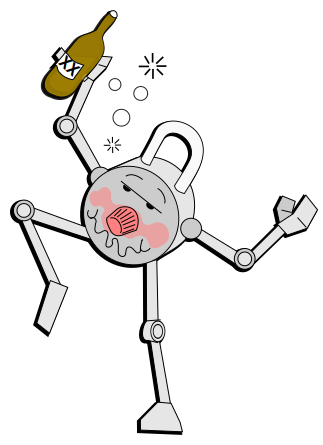
\includegraphics{cartoons/r-2014-Locking-the-Slob}}
\caption{Locking: Villain or Slob?}
\ContributedBy{Figure}{fig:locking:Locking: Villain or Slob?}{Melissa Broussard}
\end{figure}

\begin{figure}[tb]
\centering
\resizebox{2in}{!}{
\includegraphics{cartoons/r-2014-Locking-the-Hero}}
\caption{Locking: Workhorse or Hero?}
\ContributedBy{Figure}{fig:locking:Locking: Workhorse or Hero?}{Melissa Broussard}
\end{figure}

\section{Staying Alive}
\label{sec:locking:Staying Alive}

락킹이 데드락과 스타베이션으로 인해 고발당한다는 사실을 놓고 보면, 공유 메모리
병렬 프로그램 개발자들의 중요한 관심사는 그저 프로그램이 동작하는 상태를
유지하는 겁니다.
따라서 다음의 섹션들에서는 데드락, 라이브락, 스타베이션, 비공정성, 그리고
비효율성에 대해 다뤄봅니다.
\iffalse

Given that locking stands accused of deadlock and starvation,
one important concern for shared-memory parallel developers is
simply staying alive.
The following sections therefore cover deadlock, livelock, starvation,
unfairness, and inefficiency.
\fi

\subsection{Deadlock}
\label{sec:locking:Deadlock}

데드락은 한 무리의 쓰레드들이 각각 최소 하나의 락을 잡은 상태로 같은 무리의
다른 멤버가 잡고 있는 락을 놓기를 기다리고 있을 때 발생합니다.

어떤 외부의 간섭 같은 것 없이는 데드락은 영원히 존재합니다.
어떤 쓰레드도 자신이 기다리고 있는 락을 쥐고 있는 쓰레드가 그 락을 놓아주기
전까지는 얻을 수 없습니다만, 그 락을 쥐고 있는 쓰레드는 그 락을 얻기 위해
기다리고 있는 쓰레드가 쥐고 있는 락을 얻기 전까지는 자신의 락을 놓을 수
없습니다.
\iffalse

Deadlock occurs when each of a group of threads is holding at least one
lock while at the same time waiting on a lock held by a member
of that same group.

Without some sort of external intervention, deadlock is forever.
No thread can acquire the lock it is waiting on until that
lock is released by the thread holding it, but the thread holding
it cannot release it until the holding thread acquires the lock that
it is waiting on.
\fi

\begin{figure}[tb]
\centering
\resizebox{1.5in}{!}{\includegraphics{locking/DeadlockCycle}}
\caption{Deadlock Cycle}
\label{fig:locking:Deadlock Cycle}
\end{figure}

데드락 시나리오를 쓰레드와 락을 노드로 표현한 방향성이 존재하는 그래프로 표현해
볼 수 있는데, Figure~\ref{fig:locking:Deadlock Cycle} 에 그러한 표현이 그려져
있습니다.
락에서 쓰레드로의 화살표는 해당 쓰레드가 해당 락을 쥐고 있음을 의미하는데, 예를
들어 Thread~B 는 Lock~2 와~4 를 쥐고 있습니다.
쓰레드에서 락으로의 화살표는 해당 쓰레드가 해당 락을 얻기 위해 기다리고 있음을
의미하는데, 예를 들어 Thread~B 는 Lock~3 를 얻기 위해 기다리고 있습니다.

데드락 시나리오는 항상 최소한 하나 이상의 데드락 사이클을 갖게 됩니다.
Figure~\ref{fig:locking:Deadlock Cycle} 에서는 Thread~B, Lock~3, Thread~C,
Lock~4, 그리고 다시 Thread~B 로 이어지는 사이클이 존재합니다.
\iffalse

We can create a directed-graph representation of a deadlock scenario
with nodes for threads and locks, as shown in
Figure~\ref{fig:locking:Deadlock Cycle}.
An arrow from a lock to a thread indicates that the thread holds
the lock, for example, Thread~B holds Locks~2 and~4.
An arrow from a thread to a lock indicates that the thread is waiting
on the lock, for example, Thread~B is waiting on Lock~3.

A deadlock scenario will always contain at least one deadlock cycle.
In Figure~\ref{fig:locking:Deadlock Cycle}, this cycle is
Thread~B, Lock~3, Thread~C, Lock~4, and back to Thread~B.
\fi

\QuickQuiz{}
	하지만 데드락의 정의는 단지 각 쓰레드가 최소 하나 이상의 락을 잡고 일부
	쓰레드에 의해 잡혀 있는 또다른 락을 기다리고 있는 것이잖아요.
	어떻게 거기에 사이클이 존재하는지 알 수 있죠?
	\iffalse

	But the definition of deadlock only said that each thread
	was holding at least one lock and waiting on another lock
	that was held by some thread.
	How do you know that there is a cycle?
	\fi
\QuickQuizAnswer{
	그래프에 사이클이 존재하지 않는다고 생각해 봅시다.
	만약 그렇다면 우리는 방향성 비순환 그래프 (DAG: directed acyclic graph)
	를 가지게 될텐데, 이 그래프는 최소한 하나의 잎사귀 노드 (leaf node) 를
	가질 겁니다.

	이 잎사귀 노드가 락이라면, 우린 어떤 쓰레드에도 잡혀 있지 않은 락을
	기다리고 있는 한 쓰레드를 가지고 있다는 이야기가 됩니다
	(그리고 이 경우 해당 쓰레드는 즉시 해당 락을 얻게 되겠죠.)

	반면에, 만약 이 잎사귀 노드가 쓰레드였다면, 어떤 락도 기다리고 있지
	않은 쓰레드가 하나 존재한다는 이야기가 되는데, 이것 역시 데드락의
	정의를 위반합니다.
	(그리고 이 경우, 해당 쓰레드는 수행중이거나 락이 아닌 무언가에 의해
	블락되어 있거나 하는 상태일 것입니다.)

	따라서, 이 데드락의 정의에 기반하면, 앞서 설명한 데드락 상태를 나타내는
	그래프에는 사이클이 존재해야만 합니다.
	\iffalse

	Suppose that there is no cycle in the graph.
	We would then have a directed acyclic graph (DAG), which would
	have at least one leaf node.

	If this leaf node was a lock, then we would have a thread
	that was waiting on a lock that wasn't held by any thread,
	which violates the definition.
	(And in this case the thread would immediately acquire the
	lock.)

	On the other hand, if this leaf node was a thread, then
	we would have a thread that was not waiting on any lock,
	again violating the definition.
	(And in this case, the thread would either be running or
	be blocked on something that is not a lock.)

	Therefore, given this definition of deadlock, there must
	be a cycle in the corresponding graph.
	\fi
} \QuickQuizEnd

데드락 상태로부터 시스템을 복구하는 데이터베이스 시스템과 같은 소프트웨어
환경도 존재합니다만, 이런 방법은 한 쓰레드가 죽거나 락이 강제로 다른
쓰레드로부터 강탈될 수 있을 것을 필요로 합니다.
이와 같이 죽이고 강탈하는 방법은 트랜잭션들에 대해서는 적당할 수 있겠지만,
커널과 어플리케이션 수준에서의 락킹의 사용에는 많은 경우 문제가 될 수 있습니다:
그로 인해 발생하는 부분적으로만 업데이트된 구조체를 처리하는 것은 상당히
복잡하고 위험하고 오류를 만들기 쉽습니다.
\iffalse

Although there are some software environments such as database systems
that can repair an existing deadlock, this approach requires either that
one of the threads be killed or that a lock be forcibly stolen from one
of the threads.
This killing and forcible stealing can be appropriate for transactions,
but is often problematic for kernel and application-level use of locking:
dealing with the resulting partially updated structures can be extremely
complex, hazardous, and error-prone.
\fi

따라서 커널과 어플리케이션들은 데드락으로부터 회복을 하기보다는 데드락을
회피하는 방법을 사용하려 합니다.
여러개의 데드락 회피 전략이 존재하는데, 계층적 락킹
(Section~\ref{sec:locking:Locking Hierarchies}),
지역적 계층적 락킹
(Section~\ref{sec:locking:Local Locking Hierarchies}),
레이어를 사용한 계층적 락킹
(Section~\ref{sec:locking:Layered Locking Hierarchies}),
락들로의 포인터들을 갖는 API 들을 다루는 전략들
(Section~\ref{sec:locking:Locking Hierarchies and Pointers to Locks}),
조건적 락킹
(Section~\ref{sec:locking:Conditional Locking}),
필요한 락들 전체를 처음에 획득하기
(Section~\ref{sec:locking:Acquire Needed Locks First}),
한번에 하나의 락만 사용하기 설계
(Section~\ref{sec:locking:Single-Lock-at-a-Time Designs}),
그리고 시그널/인터럽트 핸들러 전략이 포함됩니다.
(Section~\ref{sec:locking:Signal/Interrupt Handlers}).
모든 상황에 완벽하게 동작하는 데드락 회피 전략이 존재하긴 합니다만, 그 중에서도
데드락 회피 도구를 잘 선택하는 방법이 있습니다.
\iffalse

Kernels and applications therefore work to avoid deadlocks rather than to
recover from them.
There are a number of deadlock-avoidance strategies,
including locking hierarchies
(Section~\ref{sec:locking:Locking Hierarchies}),
local locking hierarchies
(Section~\ref{sec:locking:Local Locking Hierarchies}),
layered locking hierarchies
(Section~\ref{sec:locking:Layered Locking Hierarchies}),
strategies for dealing with APIs containing pointers to locks
(Section~\ref{sec:locking:Locking Hierarchies and Pointers to Locks}),
conditional locking
(Section~\ref{sec:locking:Conditional Locking}),
acquiring all needed locks first
(Section~\ref{sec:locking:Acquire Needed Locks First}),
single-lock-at-a-time designs
(Section~\ref{sec:locking:Single-Lock-at-a-Time Designs}),
and strategies for signal/interrupt handlers
(Section~\ref{sec:locking:Signal/Interrupt Handlers}).
Although there is no deadlock-avoidance strategy that works perfectly
for all situations, there is a good selection of deadlock-avoidance
tools to choose from.
\fi

\subsubsection{Locking Hierarchies}
\label{sec:locking:Locking Hierarchies}

락킹 계층은 락들을 순서세워서 순서에 상관없이 락들을 획득하는 행위를 막습니다.
Figure~\ref{fig:locking:Deadlock Cycle} 의 상황에서는 한 쓰레드가 획득하려 하는
락과 같거나 더 큰 숫자의 락을 이미 쥐고 있다면 해당 그래프에서 사라지도록,
락들을 숫자에 기반한 규칙으로 순서세울 수 있을겁니다.
Thread~B 는 이 계층을 위반한 셈인데, Lock~4 를 쥔 상태에서 Lock~3 를 획득하려
하고 있기 때문이고, 이로인해 데드락이 발생했습니다.

다시 말하지만, 락킹 계층을 적용하기 위해서는 락들의 순서를 잡아주고 순서에
상관없이 락을 획득하는 행위를 막아야 합니다.
커다란 프로그램에서는 락킹 계층을 강제하기 위해 도구를 사용하는 것이 현명할
겁니다~\cite{JonathanCorbet2006lockdep}.
\iffalse

Locking hierarchies order the locks and prohibit acquiring locks out
of order.
In Figure~\ref{fig:locking:Deadlock Cycle},
we might order the locks numerically, so that a thread was
forbidden from acquiring a given lock if it already held a lock
with the same or a higher number.
Thread~B has violated this hierarchy because it is attempting to
acquire Lock~3 while holding Lock~4, which permitted the deadlock
to occur.

Again, to apply a locking hierarchy, order the locks and prohibit
out-of-order lock acquisition.
In large program, it is wise to use tools to enforce your locking
hierarchy~\cite{JonathanCorbet2006lockdep}.
\fi

\subsubsection{Local Locking Hierarchies}
\label{sec:locking:Local Locking Hierarchies}

하지만, 전역적이라는 락킹 계층의 본연적 특성은 해당 방법을 라이브러리 함수에
적용하기 어렵게 합니다.
무엇보다도, 주어진 라이브러리 함수를 사용하는 프로그램은 아직 작성되지도
않았고, 따라서 어떻게 이 불쌍한 라이브러리 함수 구현자가 아직 작성되지 않은
프로그램의 락킹 계층에 충실할 수 있기를 바랄 수 있겠어요?

다행히도 일반적인 특수한 경우가 있는데 해당 라이브러리 함수가 호출자의 코드를
전혀 사용하지 않을 때입니다.
이 경우, 호출자의 락들은 라이브러리의 락들을 잡은 상태에서 잡혀지지 않고,
따라서 라이브러리와 호출자 둘 다의 락들로부터 생성되는 데드락 사이클은 존재할
수 없습니다.
\iffalse

However, the global nature of locking hierarchies make them difficult to
apply to library functions.
After all, the program using a given library function has not even been
written yet, so how can the poor library-function implementor possibly
hope to adhere to the yet-to-be-written program's locking hierarchy?

One special case that is fortunately the common case is when
the library function does not invoke any of the caller's code.
In this case, the caller's locks will never be acquired while holding
any of the library's locks, so that there cannot be a deadlock cycle
containing locks from both the library and the caller.
\fi

\QuickQuiz{}
	이 규칙에 대한 어떤 예외가 존재해서, 라이브러리 코드가 호출자의 어떤
	함수도 실행하지 않는다는 조건 하에서도 라이브러리와 호출자 둘 다의 락을
	포함하는 데드락 사이클이 실제로는 존재할 수도 있을 수 있나요?
	\iffalse

	Are there any exceptions to this rule, so that there really could be
	a deadlock cycle containing locks from both the library and
	the caller, even given that the library code never invokes
	any of the caller's functions?
	\fi
\QuickQuizAnswer{
	실제로 존재합니다!
	여기 그런 예외들 중 일부가 있습니다:
	\iffalse

	Indeed there are!
	Here are a few of them:
	\fi
	\begin{enumerate}
	\item	라이브러리 함수의 인자 가운데 하나가 이 라이브러리 함수가
		획득하는 락으로의 포인터라면, 그리고 만약 그 라이브러리 함수가
		그 호출자의 락을 잡은 상태로 자신의 락들을 잡는다면, 호출자의
		락과 라이브러리 락들이 함께 들어간 데드락 사이클을 가질 수도
		있게 됩니다.
	\item	라이브러리 함수들 가운데 하나가 호출자에 의해 잡힌 락으로의
		포인터를 리턴하게 된다면, 그리고 만약 그 호출자가 라이브러리의
		락을 잡은 채로 자신의 락을 잡는다면, 이번에도 호출자의 락과
		라이브러리의 락들이 함께 들어간 데드락 사이클을 가질 수도 있게
		됩니다.
	\iffalse

	\item	If one of the library function's arguments is a pointer
		to a lock that this library function acquires, and if
		the library function holds one of its locks while
		acquiring the caller's lock, then we could have a
		deadlock cycle involving both caller and library locks.
	\item	If one of the library functions returns a pointer to
		a lock that is acquired by the caller, and if the
		caller acquires one of its locks while holding the
		library's lock, we could again have a deadlock
		cycle involving both caller and library locks.
	\fi
	\item	라이브러리 함수들 가운데 하나가 락을 하나 잡고 그걸 잡은채로
		리턴하게 된다면, 그리고 만약 그 호출자가 자신의 락들 가운데
		하나를 잡게 된다면, 또다시 호출자의 락과 라이브러리의 락이 모두
		연관된 데드락 사이클을 생성하는 방법이 됩니다.
	\item	호출자가 락을 잡는 시그널 핸들러를 가지고 있다면, 호출자의 락과
		라이브러리의 락이 모두 연관된 데드락 사이클이 있을 수 있습니다.
		하지만, 이 경우에 라이브러리의 락들은 데드락 사이클에 죄가 없는
		방관자일 뿐입니다.
		그렇다곤 하나, 시그널 핸들러 안에서 락을 획득하는 것은 대부분의
		환경에서 하지 말아야 할 일임을 알아두시기 바랍니다---그건 그냥
		나쁜 생각일 뿐 아니라, 지지받지 못할 일입니다.
	\iffalse

	\item	If one of the library functions acquires a lock and
		then returns while still holding it, and if the caller
		acquires one of its locks, we have yet another way
		to create a deadlock cycle involving both caller
		and library locks.
	\item	If the caller has a signal handler that acquires
		locks, then the deadlock cycle can involve both
		caller and library locks.
		In this case, however, the library's locks are
		innocent bystanders in the deadlock cycle.
		That said, please note that acquiring a lock from
		within a signal handler is a no-no in most
		environments---it is not just a bad idea, it
		is unsupported.
	\fi
	\end{enumerate}
} \QuickQuizEnd

하지만 라이브러리 함수가 실제로 호출자의 코드를 실행하는 경우를 생각해 봅시다.
예를 들어, \co{qsort()} 함수는 호출자가 제공하는 비교 함수를 실행합니다.
\co{qsort()} 의 동시적인 구현은 아마도 락킹을 사용할텐데, 이는 아마도 그러지
않을 확률이 크긴 한 케이스지만 비교 함수가 락킹에도 관여되는 좀 복잡한 함수인
경우라면 데드락을 일으킬 수 있습니다.
이 라이브러리 함수는 어떻게 데드락을 막을 수 있을까요?

이 경우에의 황금률은 ``알 수 없는 코드를 실행하기 전에 모든 락을 놓아버리기''
입니다.
이 규칙을 따르기 위해선, 앞서 언급한 \co{qsort()} 함수는 비교 함수를 실행하기
전에 모든 락을 해제해야만 합니다.
\iffalse

But suppose that a library function does invoke the caller's code.
For example, the \co{qsort()} function invokes a caller-provided
comparison function.
A concurrent implementation of \co{qsort()} likely uses locking,
which might result in deadlock in the perhaps-unlikely case where
the comparison function is a
complicated function involving also locking.
How can the library function avoid deadlock?

The golden rule in this case is ``Release all locks before invoking
unknown code.''
To follow this rule, the \co{qsort()} function must release all
locks before invoking the comparison function.
\fi

\QuickQuiz{}
	하지만 \co{qsort()} 가 비교 함수를 실행하기 전에 그 자신의 락들을 모두
	해제해버리면, 다른 \co{qsort()} 쓰레드들과의 경주 문제를 어떻게 지킬 수
	있나요?
	\iffalse

	But if \co{qsort()} releases all its locks before invoking
	the comparison function, how can it protect against races
	with other \co{qsort()} threads?
	\fi
\QuickQuizAnswer{
	비교되는 데이터 원소들을 사유화 시켜버리거나 (Chapter~\ref{chp:Data
	Ownership} 에서 설명한 것과 같이) 레퍼런스 카운팅과 같은 뒤로 미루기
	메커니즘을 사용하는 것 (Chapter~\ref{chp:Deferred Processing} 에서
	설명한 것과 같이) 으로 가능합니다.
	\iffalse

	By privatizing the data elements being compared
	(as discussed in Chapter~\ref{chp:Data Ownership})
	or through use of deferral mechanisms such as
	reference counting (as discussed in
	Chapter~\ref{chp:Deferred Processing}).
	\fi
} \QuickQuizEnd

\begin{figure}[tb]
\centering
\resizebox{3in}{!}{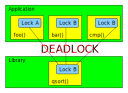
\includegraphics{locking/NonLocalLockHierarchy}}
\caption{Without Local Locking Hierarchy for \tco{qsort()}}
\label{fig:lock:Without Local Locking Hierarchy for qsort()}
\end{figure}

\begin{figure}[tb]
\centering
\resizebox{3in}{!}{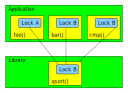
\includegraphics{locking/LocalLockHierarchy}}
\caption{Local Locking Hierarchy for \tco{qsort()}}
\label{fig:lock:Local Locking Hierarchy for qsort()}
\end{figure}

지역적 락킹 계층화의 장점을 보기 위해,
Figure~\ref{fig:lock:Without Local Locking Hierarchy for qsort()} 와
\ref{fig:lock:Local Locking Hierarchy for qsort()} 를 비교해 보시기 바랍니다.
두개의 그림에서, 어플리케이션의 함수들인 \co{foo()} 와 \co{bar()} 는 각각
Lock~A 와 B 를 잡은 상태로 \co{qsort()} 를 호출합니다.
이것은 \co{qsort()} 의 병렬화된 구현이기 때문에, 이 함수는 Lock~C 를 잡습니다.
함수 \co{foo()} 는 \co{cmp()} 함수를 \co{qsort()} 에게 전달하고, \co{cmp()}
함수는 Lock~B 를 잡습니다.
함수 \co{bar()} 는 간단한 정수 비교 함수 (그림에는 보이지 않습니다) 를
\co{qsort()} 에게 전달하고, 이 간단한 함수는 어떤 락을 잡거나 하지 않습니다.
\iffalse

To see the benefits of local locking hierarchies, compare
Figures~\ref{fig:lock:Without Local Locking Hierarchy for qsort()} and
\ref{fig:lock:Local Locking Hierarchy for qsort()}.
In both figures, application functions \co{foo()} and \co{bar()}
invoke \co{qsort()} while holding Locks~A and B, respectively.
Because this is a parallel implementation of \co{qsort()}, it acquires
Lock~C.
Function \co{foo()} passes function \co{cmp()} to \co{qsort()},
and \co{cmp()} acquires Lock~B.
Function \co{bar()} passes a simple integer-comparison function (not
shown) to \co{qsort()}, and this simple function does not acquire any
locks.
\fi

이제, \co{qsort()} 가 앞서 이야기한 모든 락을 놓기 황금률을 어기게 되어서
Figure~\ref{fig:lock:Without Local Locking Hierarchy for qsort()} 에 보인
것처럼 \co{cmp()} 를 호출하는 동안 Lock~C 를 잡고 있는다면 데드락이 일어날 수
있습니다.
이를 확실히 보기 위해, 한 쓰레드가 \co{foo()} 를 호출했고 두번째 쓰레드가
그사이 동시적으로 \co{bar()} 를 호출하는 경우를 생각해 봅시다.
첫번째 쓰레드는 Lock~A 를 잡고 두번째 쓰레드는 Lock~B 를 잡게 됩니다.
만약 첫번째 쓰레드의 \co{qsort()} 함수 호출이 Lock~C 를 잡게 된다면, 이제
\co{qsort()} 안에서 \co{cmp()} 함수를 호출했을 때 Lock~B 를 잡는 것은
불가능해집니다.
하지만 첫번째 쓰레드가 Lock~C 를 잡고 있어서 두번째 쓰레드의 \co{qsort()}
호출은 그걸 잡지 못하게 되고, 따라서 Lock~B 를 놓을 수도 없게 되므로, 데드락을
초래하게 됩니다.
\iffalse

Now, if \co{qsort()} holds Lock~C while calling \co{cmp()} in violation
of the golden release-all-locks rule above, as shown in
Figure~\ref{fig:lock:Without Local Locking Hierarchy for qsort()},
deadlock can occur.
To see this, suppose that one thread invokes \co{foo()} while a second
thread concurrently invokes \co{bar()}.
The first thread will acquire Lock~A and the second thread will acquire
Lock~B.
If the first thread's call to \co{qsort()} acquires Lock~C, then it
will be unable to acquire Lock~B when it calls \co{cmp()}.
But the first thread holds Lock~C, so the second thread's call to
\co{qsort()} will be unable to acquire it, and thus unable to release
Lock~B, resulting in deadlock.
\fi

반면에, 만약 \co{qsort()} 가 비교 함수 (\co{qsort()} 의 관점에서 보기에는 알 수
없는 코드입니다) 를 호출하기 전에 Lock~C 를 놓게 된다면, 데드락은
Figure~\ref{fig:lock:Local Locking Hierarchy for qsort()} 에 보이는 것처럼
막아집니다.

만약 각 모듈이 알 수 없는 코드를 실행하기 전에 모든 락들을 내려놓게 된다면,
그리고 각 모듈이 개별적으로 데드락을 막고 있다면 데드락은 생기지 않게 됩니다.
따라서 이 규칙은 데드락 분석을 크게 간략화 시키고 모듈성을 크게 향상시킵니다.
\iffalse

In contrast, if \co{qsort()} releases Lock~C before invoking the
comparison function, which is unknown code from \co{qsort()}'s perspective,
then deadlock is avoided as shown in
Figure~\ref{fig:lock:Local Locking Hierarchy for qsort()}.

If each module releases all locks before invoking unknown code, then
deadlock is avoided if each module separately avoids deadlock.
This rule therefore greatly simplifies deadlock analysis and greatly
improves modularity.
\fi

\subsubsection{Layered Locking Hierarchies}
\label{sec:locking:Layered Locking Hierarchies}

\begin{figure}[tb]
\centering
\resizebox{3in}{!}{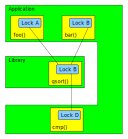
\includegraphics{locking/LayeredLockHierarchy}}
\caption{Layered Locking Hierarchy for \tco{qsort()}}
\label{fig:lock:Layered Locking Hierarchy for qsort()}
\end{figure}

불행하게도, \co{qsort()} 가 자신의 모든 락들을 앞서 이야기한 비교 함수를
호출하기 전에 해제하는 것은 불가능할 수 있습니다.
이런 경우, 알 수 없는 코드를 실행하기 전에 모든 락들을 해제하는 지역적 락킹
계층을 사용할 수 없습니다.
하지만, 그 대신에 층을 이룬 락킹 계층을 사용할 수 있는데, 이 방법은
Figure~\ref{fig:lock:Layered Locking Hierarchy for qsort()} 에 그려져 있습니다.
여기서, \co{cmp()} 함수는 Lock~A, B, C 가 잡힌 이후에 새로운 Lock~D 를
사용함으로써 데드락을 막습니다.
따라서 전역적인 데드락 계층에 세개의 층이 존재하는 셈인 것으로, 첫번째 층은
Lock~A 와 B 에, 그리고 두번째 층은 Lock~C 를 가지며, 세번째 층은 Lock~D 를
포함합니다.
\iffalse

Unfortunately, it might not be possible for \co{qsort()} to release
all of its locks before invoking the comparison function.
In this case, we cannot construct a local locking hierarchy by
releasing all locks before invoking unknown code.
However, we can instead construct a layered locking hierarchy, as shown in
Figure~\ref{fig:lock:Layered Locking Hierarchy for qsort()}.
here, the \co{cmp()} function uses a new Lock~D that is acquired after
all of Locks~A, B, and C, avoiding deadlock.
we therefore have three layers to the global deadlock hierarchy, the
first containing Locks~A and B, the second containing Lock~C, and
the third containing Lock~D.
\fi

\begin{listing}[tbp]
{ \scriptsize
\begin{verbbox}
  1 struct locked_list {
  2   spinlock_t s;
  3   struct list_head h;
  4 };
  5 
  6 struct list_head *list_start(struct locked_list *lp)
  7 {
  8   spin_lock(&lp->s);
  9   return list_next(lp, &lp->h);
 10 }
 11 
 12 struct list_head *list_next(struct locked_list *lp,
 13                             struct list_head *np)
 14 {
 15   struct list_head *ret;
 16 
 17   ret = np->next;
 18   if (ret == &lp->h) {
 19     spin_unlock(&lp->s);
 20     ret = NULL;
 21   }
 22   return ret;
 23 }
\end{verbbox}
}
\centering
\theverbbox
\caption{Concurrent List Iterator}
\label{lst:locking:Concurrent List Iterator}
\end{listing}

\co{cmp()} 함수가 새로운 락인 Lock~D 를 사용하도록 수정하는 것을 기계적으로
하는 건 일반적으로 불가능하다는 것을 알아 두시기 바랍니다.
오히려 그 반대입니다: 그러한 변경을 위해서는 대부분의 경우 기초적인 설계
레벨에서의 수정을 필요로 하게 됩니다.
하지만 더도 아니고 덜도 아니고, 그런 변경을 위해 필요한 노력은 일반적으로
데드락을 막기 위해서 치뤄야 하는 대가 치고는 적은 편입니다.

알 수 없는 코드를 실행하기 전에 모든 락을 해제하는 것이 비현실적인 또다른 예를
들어보기 위해서는,
Listing~\ref{lst:locking:Concurrent List Iterator} (\co{locked_list.c}) 에
보여진 것과 같이 링크드 리스트를 순회하는 반복자 (iterator) 를 생각해 보시기
바랍니다.
\co{list_start()} 함수는 리스트의 락을 잡고서 첫번째 원소를 리턴하고 (원소가
존재한다면), \co{list_next()} 함수는 리스트의 그 다음 원소로의 포인터를
리턴하는데, 리스트의 끝에 도달한 경우에는 앞서 잡았던 락을 해제하고 \co{NULL}
을 리턴합니다.
\iffalse

Please note that it is not typically possible to mechanically
change \co{cmp()} to use the new Lock~D.
Quite the opposite: It is often necessary to make profound design-level
modifications.
Nevertheless, the effort required for such modifications is normally
a small price to pay in order to avoid deadlock.

For another example where releasing all locks before invoking unknown
code is impractical, imagine an iterator over a linked list, as shown in
Listing~\ref{lst:locking:Concurrent List Iterator} (\path{locked_list.c}).
The \co{list_start()} function acquires a lock on the list and returns
the first element (if there is one), and
\co{list_next()} either returns a pointer to the next element in the list
or releases the lock and returns \co{NULL} if the end of the list has
been reached.
\fi

\begin{listing}[tbp]
{ \scriptsize
\begin{verbbox}
  1 struct list_ints {
  2   struct list_head n;
  3   int a;
  4 };
  5 
  6 void list_print(struct locked_list *lp)
  7 {
  8   struct list_head *np;
  9   struct list_ints *ip;
 10 
 11   np = list_start(lp);
 12   while (np != NULL) {
 13     ip = list_entry(np, struct list_ints, n);
 14     printf("\t%d\n", ip->a);
 15     np = list_next(lp, np);
 16   }
 17 }
\end{verbbox}
}
\centering
\theverbbox
\caption{Concurrent List Iterator Usage}
\label{lst:locking:Concurrent List Iterator Usage}
\end{listing}

Listing~\ref{lst:locking:Concurrent List Iterator Usage} 는 이 리스트 반복자가
어떻게 사용될 수 있는지 보여줍니다.
Line~1-4 는 하나의 정수를 포함하는 \co{list_ints} 원소를 정의하고 line~6-17
에서는 이 원소가 포함된 리스트에의 순회를 어떻게 반복하는지 보입니다.
Line~11 에서는 이 리스트를 잠그고 첫번째 원소로의 포인터를 얻어온 후, line~13
에서 해당 원소에 동봉되어 있는 \co{list_ints} 구조체로의 포인터를 얻어오고,
line~14 에서 연관된 정수를 출력하고서, line~15 에서 다음 원소로 넘어갑니다.
이 코드는 상당히 간단하고, 락킹을 모두 숨겼습니다.
\iffalse

Listing~\ref{lst:locking:Concurrent List Iterator Usage} shows how
this list iterator may be used.
Lines~1-4 define the \co{list_ints} element containing a single integer,
and lines~6-17 show how to iterate over the list.
Line~11 locks the list and fetches a pointer to the first element,
line~13 provides a pointer to our enclosing \co{list_ints} structure,
line~14 prints the corresponding integer, and
line~15 moves to the next element.
This is quite simple, and hides all of the locking.
\fi

각 리스트의 원소를 처리하는 코드가 그 스스로 \co{list_start()} 나
\co{list_next()} 를 호출하는 다른 코드와 함께 사용하는, 데드락을 초래할 수
있는, 락을 사용하지 않는한은 이 락킹은 계속 숨겨져 있을 수 있습니다.
이렇게 리스트 반복자 락킹을 구현하면서 데드락을 막기 위해 락킹 계층을 여러
레이어에 층층이 놓을 수 있습니다.

이 층쌓기 방법은 임의의 많은 수의 레이어들로 확장될 수도 있습니다만, 각각의
추가된 레이어는 락킹 설계의 복잡도를 증가시킵니다.
그런 증가된 복잡도는 특히 객체지향적 설계의 어떤 타입들에는 불편할 수 있는데,
코드의 제어와 수행이 많은 수의 객체들 사이를 규칙이 정해지지 않은 형태로 왔다
갔다 하게 되는 경우가 그런 경우입니다.\footnote{
	이런 것들을 일컫기를 ``객체지향적 스파게티 코드'' 라고 합니다.}
이런 객체지향적 설계의 습관들과 데드락 회피의 필요성 사이의 미스매치는 병렬
프로그래밍이 어떤 사람들에게는 매우 어렵다고 인지되는데 대한 심각한 이유입니다.

수많은 레이어를 사용하는 락킹 계층들에 대한 일부 대안책은
Chapter~\ref{chp:Deferred Processing} 에서 다뤄집니다.
\iffalse

That is, the locking remains hidden as long as the code processing each
list element does not itself acquire a lock that is held across some
other call to \co{list_start()} or \co{list_next()}, which results in
deadlock.
We can avoid the deadlock by layering the locking hierarchy
to take the list-iterator locking into account.

This layered approach can be extended to an arbitrarily large number of layers,
but each added layer increases the complexity of the locking design.
Such increases in complexity are particularly inconvenient for some
types of object-oriented designs, in which control passes back and forth
among a large group of objects in an undisciplined manner.\footnote{
	One name for this is ``object-oriented spaghetti code.''}
This mismatch between the habits of object-oriented design and the
need to avoid deadlock is an important reason why parallel programming
is perceived by some to be so difficult.

Some alternatives to highly layered locking hierarchies are covered in
Chapter~\ref{chp:Deferred Processing}.
\fi

\subsubsection{Locking Hierarchies and Pointers to Locks}
\label{sec:locking:Locking Hierarchies and Pointers to Locks}

일부 예외가 있긴 하지만, 락으로의 포인터를 갖는 외부의 API 는 대부분의 경우
잘못 설계된 API 입니다.
내부의 락을 어떤 다른 소프트웨어 컴포넌트에서 처리하는 것은 일단 정보
은닉이라는 핵심 설계 원칙에 위배되는 행위입니다.
\iffalse

Although there are some exceptions, an external API containing a pointer
to a lock is very often a misdesigned API.
Handing an internal lock to some other software component is after all
the antithesis of information hiding, which is in turn a key design
principle.
\fi

\QuickQuiz{}
	락으로의 포인터를 함수에 넘기는 게 완벽하게 합리적인 예외를 하나만 들어
	보세요.
	\iffalse

	Name one common exception where it is perfectly reasonable
	to pass a pointer to a lock into a function.
	\fi
\QuickQuizAnswer{
	락킹 도구들이죠, 당연히!
	\iffalse

	Locking primitives, of course!
	\fi
} \QuickQuizEnd

예외 가운데 하나는 어떤 것을 떠맡게 되는 함수들인데, 호출자의 락은 떠맡기기
하기 전에 반드시 잡혀야만 하지만 그 락은 해당 함수가 리턴하기 전에는
해제되어야만 하는 경우입니다.
그런 함수의 한 예는 POSIX \co{pthread_cond_wait()} 와 같은 함수가 될텐데,
\co{pthread_mutex_t} 로의 포인터를 넘김으로써 일어날 조건을 놓쳐서 계속 깨어날
조건을 기다리고만 있게 되는 일을 방지합니다.
\iffalse

One exception is functions that hand off some entity,
where the caller's lock must be held until the handoff is complete,
but where the lock must be released before the function returns.
One example of such a function is the POSIX \co{pthread_cond_wait()}
function, where passing an pointer to a \co{pthread_mutex_t}
prevents hangs due to lost wakeups.
\fi

\QuickQuiz{}
	\co{pthread_cond_wait()} 함수가 먼저 그 뮤텍스를 해제하고 나서 다시
	획득한다는 사실은 데드락의 가능성을 제거하는 거 아닌가요?
	\iffalse

	Doesn't the fact that \co{pthread_cond_wait()} first releases the
	mutex and then re-acquires it eliminate the possibility of deadlock?
	\fi
\QuickQuizAnswer{
	전혀 그렇지 않습니다!

	\co{mutex_a} 를 획득하고, 그 후엔 \co{mutex_b} 를 획득하고 나서는
	\co{mutex_a} 를 \co{pthread_cond_wait} 에 넘겨버리는 한 프로그램을
	생각해 보세요.
	이제 \co{pthread_cond_wait} 는 \co{mutex_a} 를 해제합니다만, 리턴하기
	전에 그걸 다시 잡습니다.
	만약 그 사이에 다른 쓰레드가 \co{mutex_a} 를 잡고서 \co{mutex_b} 를
	사용해 블락된다면, 이 프로그램은 데드락에 빠지고 맙니다.
	\iffalse

	Absolutely not!

	Consider a program that acquires \co{mutex_a}, and then
	\co{mutex_b}, in that order, and then passes \co{mutex_a}
	to \co{pthread_cond_wait}.
	Now, \co{pthread_cond_wait} will release \co{mutex_a}, but
	will re-acquire it before returning.
	If some other thread acquires \co{mutex_a} in the meantime
	and then blocks on \co{mutex_b}, the program will deadlock.
	\fi
} \QuickQuizEnd

다시 말해, 어떤 락으로의 포인터를 인자로 받거나 리턴 값으로 취하는 API 를
외부로 노출하고자 한다면 그 API 설계를 다시한번 조심스럽게 고려해 보시기
바랍니다.
그건 해야만 할 옳은 일일수도 있을지 모르겠습니다만, 그간의 경험은 그렇지 않을
가능성이 높음을 이야기 합니다.
\iffalse

In short, if you find yourself exporting an API with a pointer to a
lock as an argument or the return value, do yourself a favor and carefully
reconsider your API design.
It might well be the right thing to do, but experience indicates that
this is unlikely.
\fi

\subsubsection{Conditional Locking}
\label{sec:locking:Conditional Locking}

\begin{listing}[tbp]
{ \scriptsize
\begin{verbbox}
  1 spin_lock(&lock2);
  2 layer_2_processing(pkt);
  3 nextlayer = layer_1(pkt);
  4 spin_lock(&nextlayer->lock1);
  5 layer_1_processing(pkt);
  6 spin_unlock(&lock2);
  7 spin_unlock(&nextlayer->lock1);
\end{verbbox}
}
\centering
\theverbbox
\caption{Protocol Layering and Deadlock}
\label{lst:locking:Protocol Layering and Deadlock}
\end{listing}

하지만 합리적인 락킹 계층이 존재하지 않는다고 생각해 봅시다.
이런 상황은 실제 세상에 존재할 수 있는데, 예를 들어보자면 패킷이 양방향에서
오가는 계층적 네트워크 프로토콜 스택을 생각해 볼 수 있겠습니다.
이 네트워킹의 경우, 한 패킷을 한 계층에서 다른 계층으로 보내고자 할 때 양
계층에서 모두 락을 잡아야 할 필요가 있을 수 있습니다.
패킷들은 이 프로토콜 스택의 위로도 아래로도 이동될 수 있다는 점을 생각해 보면, 
Listing~\ref{lst:locking:Protocol Layering and Deadlock} 에 보여진 것처럼
데드락을 유발하기 위한 좋은 방법입니다.
여기서, 랜선을 향해 스택의 아래 방향으로 이동하게 되는 패킷은 다음 계층의 락을
위에서 아래 순서대로 잡아야만 합니다.
랜선으로부터 스택의 위 방향으로 이동하게 되는 패킷들은 그 락들을 아래에서 위
순서대로 잡아야 한다는 점을 상기해 보면, 해당 그림의 line~4 에서의 락 획득은
데드락을 초래할 수 있습니다.
\iffalse

But suppose that there is no reasonable locking hierarchy.
This can happen in real life, for example, in layered network protocol stacks
where packets flow in both directions.
In the networking case, it might be necessary to hold the locks from
both layers when passing a packet from one layer to another.
Given that packets travel both up and down the protocol stack, this
is an excellent recipe for deadlock, as illustrated in
Listing~\ref{lst:locking:Protocol Layering and Deadlock}.
Here, a packet moving down the stack towards the wire must acquire
the next layer's lock out of order.
Given that packets moving up the stack away from the wire are acquiring
the locks in order, the lock acquisition in line~4 of the listing
can result in deadlock.
\fi

\begin{listing}[tbp]
{ \scriptsize
\begin{verbbox}
  1 retry:
  2   spin_lock(&lock2);
  3   layer_2_processing(pkt);
  4   nextlayer = layer_1(pkt);
  5   if (!spin_trylock(&nextlayer->lock1)) {
  6     spin_unlock(&lock2);
  7     spin_lock(&nextlayer->lock1);
  8     spin_lock(&lock2);
  9     if (layer_1(pkt) != nextlayer) {
 10       spin_unlock(&nextlayer->lock1);
 11       spin_unlock(&lock2);
 12       goto retry;
 13     }
 14   }
 15   layer_1_processing(pkt);
 16 spin_unlock(&lock2);
 17 spin_unlock(&nextlayer->lock1);
\end{verbbox}
}
\centering
\theverbbox
\caption{Avoiding Deadlock Via Conditional Locking}
\label{lst:locking:Avoiding Deadlock Via Conditional Locking}
\end{listing}

이 경우에 데드락을 막을 수 있는 한가지 방법은 락킹 계층을 적용하되, 락을 위에서
아래 순서로 잡아야 할 경우에는 
Listing~\ref{lst:locking:Avoiding Deadlock Via Conditional Locking} 에 보인
것처럼 조건적으로 잡는 것입니다.
무조건적으로 layer-1 락을 획득하는 대신에, line~5 에서는 그 락을
\co{spin_trylock()} 기능을 사용해 조건적으로 획득합니다.
이 기능은 만약 락이 획득 가능하다면 곧바로 락을 획득해 버리고 (0 이 아닌 값을
리턴합니다), 그렇지 않다면 락을 잡지 않고 0을 리턴합니다.
\iffalse

One way to avoid deadlocks in this case is to impose a locking hierarchy,
but when it is necessary to acquire a lock out of order, acquire it
conditionally, as shown in
Listing~\ref{lst:locking:Avoiding Deadlock Via Conditional Locking}.
Instead of unconditionally acquiring the layer-1 lock, line~5
conditionally acquires the lock using the \co{spin_trylock()} primitive.
This primitive acquires the lock immediately if the lock is available
(returning non-zero), and otherwise returns zero without acquiring the lock.
\fi

만약 \co{spin_trylock()} 이 성공했다면, line~15 는 필요한 layer-1 의 처리를
진행합니다.
그렇지 않다면, line~6 에서 락을 해제하고 line~7 과 8 에서 올바른 순서대로 그
락들을 다시 잡습니다.
불행히도, 시스템에는 여러 네트워킹 디바이스들이 존재할 수 있는데 (예: 이더넷과
WiFi), 따라서 \co{layer_1()} 함수는 라우팅 결정을 해야만 합니다.
이 결정은 언제든 바뀔 수도 있는데, 특히 그 시스템이 모바일 기기라면 더욱
그렇습니다.\footnote{
	그리고, 1900년대와는 다르게, 모바일 기기는 상당히 흔해졌죠.}
따라서, line~9 는 그 결정을 다시 한번 체크해 봐야 하고, 바뀌었다면 그 락들을
놓고 일을 처음부터 다시 시작해야 합니다.
\iffalse

If \co{spin_trylock()} was successful, line~15 does the needed
layer-1 processing.
Otherwise, line~6 releases the lock, and lines~7 and 8 acquire them in
the correct order.
Unfortunately, there might be multiple networking devices on
the system (e.g., Ethernet and WiFi), so that the \co{layer_1()}
function must make a routing decision.
This decision might change at any time, especially if the system
is mobile.\footnote{
	And, in contrast to the 1900s, mobility is the common case.}
Therefore, line~9 must recheck the decision, and if it has changed,
must release the locks and start over.
\fi

\QuickQuiz{}
	Listing~\ref{lst:locking:Protocol Layering and Deadlock} 에서
	Listing~\ref{lst:locking:Avoiding Deadlock Via Conditional Locking} 로의
	변경이 어디서나 적용될 수 있는 걸까요?
	\iffalse

	Can the transformation from
	Listing~\ref{lst:locking:Protocol Layering and Deadlock} to
	Listing~\ref{lst:locking:Avoiding Deadlock Via Conditional Locking}
	be applied universally?
	\fi
\QuickQuizAnswer{
	절대 그렇지 않습니다!

	이 변경은 \co{layer_2_processing()} 함수가 같은 입력에 대해선 항상 같은
	출력을 내놓는다는 가정을 가지고 있는데, \co{layer_1()} 의 라우팅 결정이
	변화되면 같은 패킷에 대해 이 함수가 여러번 수행될 수도 있기 때문입니다.
	따라서, 실제 세상에서 이런 변경을 적용하기는 상당히 복잡해질 수
	있습니다.
	\iffalse

	Absolutely not!

	This transformation assumes that the
	\co{layer_2_processing()} function is idempotent, given that
	it might be executed multiple times on the same packet when
	the \co{layer_1()} routing decision changes.
	Therefore, in real life, this transformation can become
	arbitrarily complex.
	\fi
} \QuickQuizEnd

\QuickQuiz{}
	그렇지만
	Listing~\ref{lst:locking:Avoiding Deadlock Via Conditional Locking}
	에서의 추가된 복잡도는 그게 데드락을 막는다는 점을 생각하면 꽤 가치있는
	거예요, 맞죠?
	\iffalse

	But the complexity in
	Listing~\ref{lst:locking:Avoiding Deadlock Via Conditional Locking}
	is well worthwhile given that it avoids deadlock, right?
	\fi
\QuickQuizAnswer{
	아마도요.

	만약 \co{layer_1()} 에서의 라우팅 결정이 충분히 자주 바뀐다면, 해당
	코드는 항상 재시도만 할테고, 진전은 전혀 이루지 못할 겁니다.
	이런 현상을 가리켜 어떤 쓰레드도 진행을 못하고 있을 때에는 ``livelock''
	이라 하고, 일부 쓰레드는 진행을 이루고 있지만 다른 것들은 못하고 있을
	때에는 ``starvation'' 이라 합니다 (Section~\ref{sec:locking:Livelock
	and Starvation} 을 참고하세요).
	\iffalse

	Maybe.

	If the routing decision in \co{layer_1()} changes often enough,
	the code will always retry, never making forward progress.
	This is termed ``livelock'' if no thread makes any forward progress or
	``starvation''
	if some threads make forward progress but others do not
	(see Section~\ref{sec:locking:Livelock and Starvation}).
	\fi
} \QuickQuizEnd

\subsubsection{Acquire Needed Locks First}
\label{sec:locking:Acquire Needed Locks First}

조건적 락킹의 중요하고 특수한 한 케이스에는 모든 필요한 락들이 추후의 작업
진행을 이루기 전에 획득됩니다.
이런 경우에, 처리하는 일이 멱등성을 가질 필요는 없습니다: 이미 쥐고 있는 락들
가운데 하나를 먼저 놓지 않고는 어떤 락을 잡는 것이 불가능함이 밝혀진다면, 그냥
모든 락을 놓아버리고 다시 락 획득을 시도합니다.
모든 필요한 락들을 한번이라도 모두 잡기만 한다면 추후의 작업이 진행됩니다.

하지만, 이런 처리 방법은 \emph{livelock} 을 초래할 수 있는데, 이에 대해서는
Section~\ref{sec:locking:Livelock and Starvation} 에서 이야기 합니다.
\iffalse

In an important special case of conditional locking all needed
locks are acquired before any processing is carried out.
In this case, processing need not be idempotent: if it turns out
to be impossible to acquire a given lock without first releasing
one that was already acquired, just release all the locks and
try again.
Only once all needed locks are held will any processing be carried out.

However, this procedure can result in \emph{livelock}, which will
be discussed in
Section~\ref{sec:locking:Livelock and Starvation}.
\fi

\QuickQuiz{}
	Section~\ref{sec:locking:Acquire Needed Locks First} 에서 이야기한
	``필요한 락들을 먼저 획득하기'' 방법을 사용할 때에, 어떻게 하면
	livelock 을 막을 수 있을까요?
	\iffalse

	When using the ``acquire needed locks first'' approach described in
	Section~\ref{sec:locking:Acquire Needed Locks First},
	how can livelock be avoided?
	\fi
\QuickQuizAnswer{
	추가적인 글로벌 락을 제공하는 겁니다.
	어떤 쓰레드가 반복적으로 필요한 락들을 획득하려 노력하고 실패했다면 그
	쓰레드는 조건없이 새로운 글로벌 락을 획득하도록 하고 조건없이 모든
	필요한 락들을 획득하게 하는 겁니다.
	(Doug Lea. 에 의해 제안된 방법입니다.)
	\iffalse

	Provide an additional global lock.
	If a given thread has repeatedly tried and failed to acquire the needed
	locks, then have that thread unconditionally acquire the new
	global lock, and then unconditionally acquire any needed locks.
	(Suggested by Doug Lea.)
	\fi
} \QuickQuizEnd

관련된 방법으로 two-phase 락킹~\cite{PhilipABernstein1987} 이 있는데, 이 방법은
트랜잭션을 제공하는 상용 수준의 데이터베이스 시스템들에서 오랫동안 사용되어
왔습니다.
Two-phase 락킹 트랜잭션의 첫번째 페이스 (phase) 에서는 락들은 획득은 되지만
해제는 되지 않습니다.
모든 필요한 락들이 획득된다면, 이 트랜잭션은 두번째 페이스로 들어가게 되는데,
이 페이스에서는 락들이 해제만 되지, 획득은 되지 않습니다.
이 락킹 방법은 데이터베이스들이 serializability 를 트랜잭션들에게 보장해줄 수
있게 하는데, 달리 말하자면, 트랜잭션들에 의해 만들어지고 보여지는 모든 값들이
모든 트랜잭션들의 어떤 전체적인 순서에 대해 일관적이게 될 것을 보장해 주기 위해
사용됩니다.
그런 많은 시스템들은 트랜잭션들을 중단 (abort) 시킬 수 있는 기능에 의존하는데,
사실 모든 필요한 락들이 획득되기 전까지는 공유된 데이터에 어떤 변경도 가하지
않도록 하는 것으로 단순화 시킬 수도 있습니다.
Livelock 과 deadlock 은 그런 시스템들에서의 문제거리들인데, 실용적인 해결책들은
많은 데이터베이스 서적들에서 찾을 수 있을 겁니다.
\iffalse

A related approach, two-phase locking~\cite{PhilipABernstein1987},
has seen long production use in transactional database systems.
In the first phase of a two-phase locking transaction, locks are
acquired but not released.
Once all needed locks have been acquired, the transaction enters the
second phase, where locks are released, but not acquired.
This locking approach allows databases to provide serializability
guarantees for their transactions, in other words, to guarantee
that all values seen and produced by the transactions are consistent
with some global ordering of all the transactions.
Many such systems rely on the ability to abort transactions, although
this can be simplified by avoiding making any changes to shared data
until all needed locks are acquired.
Livelock and deadlock are issues in such systems, but practical
solutions may be found in any of a number of database textbooks.
\fi

\subsubsection{Single-Lock-at-a-Time Designs}
\label{sec:locking:Single-Lock-at-a-Time Designs}

어떤 경우에는, 락들을 다른 락 안에 넣는 것을 막을 수 있는데, 따라서 데드락을
막을 수 있습니다.
예를 들어, 만약 문제가 완벽하게 분리될 수 있는 성질의 것이라면, 각 분리된
파티션에 하나의 락을 각각 할당할 수 있을 겁니다.
이렇게 되면 하나의 주어진 파티션을 작업하는 쓰레드는 그에 연관된 락 하나만을
잡으면 됩니다.
어떤 쓰레드도 한번에 하나 이상의 락을 잡지는 않으므로, 데드락은 발생할 수
없습니다.

하지만, 어떤 락도 잡혀있지 않은 때에도 필요한 데이터 구조체들은 존재함을
보장해줄 어떤 메커니즘이 반드시 있어야만 합니다.
그런 메커니즘 가운데 하나를 Section~\ref{sec:locking:Lock-Based Existence
Guarantees} 에서 이야기 해보고, Chapter~\ref{chp:Deferred Processing} 에서 그
외에 몇가지 다른 메커니즘들을 살펴봅니다.
\iffalse

In some cases, it is possible to avoid nesting locks, thus avoiding
deadlock.
For example, if a problem is perfectly partitionable, a single
lock may be assigned to each partition.
Then a thread working on a given partition need only acquire the one
corresponding lock.
Because no thread ever holds more than one lock at a time,
deadlock is impossible.

However, there must be some mechanism to ensure that the needed data
structures remain in existence during the time that neither lock is
held.
One such mechanism is discussed in
Section~\ref{sec:locking:Lock-Based Existence Guarantees}
and several others are presented in
Chapter~\ref{chp:Deferred Processing}.
\fi

\subsubsection{Signal/Interrupt Handlers}
\label{sec:locking:Signal/Interrupt Handlers}

시그널 핸들러와 연관된 데드락들은 시그널 핸들러 안에서
\co{pthread_mutex_lock()} 함수를 호출하는 것은 허용되지 않는 행위라는 것을
알리는 것만으로도 빠르게 없앨 수 있습니다~\cite{OpenGroup1997pthreads}.
하지만, 시그널 핸들러 안에서 사용될 수 있는 손으로 만든 락킹 도구 (대부분의
경우 지혜롭지 못한 행동입니다만) 를 사용할 가능성도 존재합니다.
그와는 별개로, 모든 운영체제 커널들은 커널에서는 시그널 핸들러라는 유사한
이름으로 다뤄지는 인터럽트 핸들러 안에서의 락 획득을 허가합니다.

여기서의 트릭은 인터럽트 핸들러 안에서 잡을 수도 있는 락이라면 어떤 락이든지
잡을 때마다 시그널들을 막아버리는 (또는, 경우에 따라서, 인터럽트를 무효화 시킬
수도 있습니다) 겁니다.
더 나아가서, 그런 락을 잡고 있다면, 시그널들을 블락시키지 않은채로 시그널
핸들러 밖에서 한번이라도 잡은 적 있는 락을 잡으려는 시도 역시 해선 안됩니다.
\iffalse

Deadlocks involving signal handlers are often quickly dismissed by
noting that it is not legal to invoke \co{pthread_mutex_lock()} from
within a signal handler~\cite{OpenGroup1997pthreads}.
However, it is possible (though almost always unwise) to hand-craft
locking primitives that can be invoked from signal handlers.
Besides which, almost all operating-system kernels permit locks to
be acquired from within interrupt handlers, which are the kernel analog
to signal handlers.

The trick is to block signals (or disable interrupts, as the case may be)
when acquiring any lock that might be acquired within an interrupt
handler.
Furthermore, if holding such a lock, it is illegal to attempt to
acquire any lock that is ever acquired
outside of a signal handler without blocking signals.
\fi

\QuickQuiz{}
	시그널 핸들러 안에서 획득되는 Lock~B 를 잡은 채로 시그널들을 블락시키지
	않고 시그널 핸들러 밖에서 획득되는 Lock~A 를 잡는 행위가 해선 안되는
	행위이죠?
	\iffalse
	Why is it illegal to acquire a Lock~A that is acquired outside
	of a signal handler without blocking signals while holding
	a Lock~B that is acquired within a signal handler?
	\fi
\QuickQuizAnswer{
	데드락을 유발할 수 있기 때문입니다.
	Lock~A 가 시그널들을 블락시키지 않은 상태로 시그널 핸들러의 밖에서
	잡혔다면, 이 락을 잡고 있는 상태로 어떤 시그널은 처리될 수 있을 겁니다.
	이제 그 시그널에 연관된 시그널 핸들러는 Lock~B 를 잡으려 할텐데, 따라서
	Lock~B 는 Lock~A 를 잡은채로 획득될 것입니다.
	따라서, 질문에서 이야기한 것처럼 우리가 Lock~B 를 잡은 채로 Lock~A 를
	잡으려 한다면 데드락 사이클이 생기게 되는 것입니다.

	따라서, 시그널 핸들러 안에서 획득하는 락을 잡고 시그널들을 블락시키지
	않은채로 시그널 핸들러 밖에서 획득되는 락을 잡는 행위는 금지된
	행위입니다.
	\iffalse

	Because this would lead to deadlock.
	Given that Lock~A is held outside of a signal
	handler without blocking signals, a signal might be handled while
	holding this lock.
	The corresponding signal handler might then acquire
	Lock~B, so that Lock~B is acquired while holding Lock~A.
	Therefore, if we also acquire Lock~A while holding Lock~B
	as called out in the question, we will have a deadlock cycle.

	Therefore, it is illegal to acquire a lock that is acquired outside
	of a signal handler without blocking signals while holding
	a another lock that is acquired within a signal handler.
	\fi
} \QuickQuizEnd

일부 시그널들을 위한 핸들러들에서 한 락을 잡았다면, 그 시그널들 모두는 그 락이
획득될 때마다, 심지어 그 락이 시그널 핸들러 안에서 잡힐 때 조차도 블락되어야만
합니다.
\iffalse

If a lock is acquired by the handlers for several signals, then each
and every one of these signals must be blocked whenever that lock is
acquired, even when that
lock is acquired within a signal handler.
\fi

\QuickQuiz{}
	시그널 핸들러 안에서 어떻게 시그널들을 블락시킬 수가 있죠?
	\iffalse

	How can you legally block signals within a signal handler?
	\fi
\QuickQuizAnswer{
	그렇게 할 수 있는 가장 간단하고 가장 빠른 방법은 시그널을 설정할 때
	\co{sigaction()} 함수에 전달하는 \co{struct sigaction} 객체의
	\co{sa_mask} 필드를 사용하는 겁니다.
	\iffalse

	One of the simplest and fastest ways to do so is to use
	the \co{sa_mask} field of the \co{struct sigaction} that
	you pass to \co{sigaction()} when setting up the signal.
	\fi
} \QuickQuizEnd

안타깝게도, 시그널들을 블락하고 블락 해제하는 행위는 일부 운영체제에서는 많은
비용을 필요로 할 수 있는데, 특히 리눅스도 포함되고, 따라서 성능에 주안점을
둔다는 말은 곧 시그널 핸들러들 안에서 획득되는 락들은 시그널 핸들러들 안에서만
획득되며, 어플리케이션 코드와 시그널 핸들러 사이의 통신에는 락을 사용하지 않는
동기화 메커니즘만을 사용한다는 의미가 되곤 합니다.

또는 치명적인 문제 상황을 처리하기 위한 경우를 제외하고는 시그널 핸들러를 아예
사용하지 않는 방법도 있습니다.
\iffalse

Unfortunately, blocking and unblocking signals can be expensive in
some operating systems, notably including Linux, so performance
concerns often mean that locks acquired in signal handlers are only
acquired in signal handlers, and that lockless synchronization
mechanisms are used to communicate between application code and
signal handlers.

Or that signal handlers are avoided completely except for handling
fatal errors.
\fi

\QuickQuiz{}
	시그널 핸들러들 안에서 락을 잡는 행위가 그렇게 나쁜 생각이라면, 그걸
	안전하게 해내기 위한 생각 자체는 대체 왜 하는거죠?
	\iffalse

	If acquiring locks in signal handlers is such a bad idea, why
	even discuss ways of making it safe?
	\fi
\QuickQuizAnswer{
	똑같은 규칙이 운영체제 커널들과 일부 임베디드 어플리케이션들에서
	사용되는 인터럽트 핸들러들에도 적용되기 때문입니다.
	\iffalse

	Because these same rules apply to the interrupt handlers used in
	operating-system kernels and in some embedded applications.
	\fi

	많은 어플리케이션 환경에서, 시그널 핸들러 안에서 락을 잡으려 하는
	행위는 해로운 행위로 여겨져 왔습니다~\cite{OpenGroup1997pthreads}.
	하지만, 그런 분위기가 똑똑한 개발자들이 (보통은 현명하지 못한 짓이지만)
	어토믹 오퍼레이션들을 사용해서 직접 만든 락들을 사용해대는 것을 멈추게
	하지는 않았습니다.
	그리고 어토믹 오퍼레이션들은 많은 경우 시그널 핸들러 안에서 사용되어도
	전혀 문제가 되지 않습니다.
	\iffalse

	In many application environments, acquiring locks in signal
	handlers is frowned upon~\cite{OpenGroup1997pthreads}.
	However, that does not stop clever developers from (usually
	unwisely) fashioning home-brew locks out of atomic operations.
	And atomic operations are in many cases perfectly legal in
	signal handlers.
	\fi
} \QuickQuizEnd

\subsubsection{Discussion}
\label{sec:locking:Locking Hierarchy Discussion}

공유 메모리 병렬 프로그래머가 사용할 수 있는 수많은 데드락 방지 전략이
존재합니다만 그 중 어느것도 잘 들어맞지 않는 순차적 프로그램들도 존재하지요.
이게 전문적인 프로그래머들이라면 자신의 도구상자에 두개 이상의 도구를 갖추고
있는 이유입니다: 락킹은 훌륭한 동시성 제어 도구이지만, 다른 도구들을 가지고
다룰 수 있는 일들도 많습니다.
\iffalse

There are a large number of deadlock-avoidance strategies available to
the shared-memory parallel programmer, but there are sequential
programs for which none of them is a good fit.
This is one of the reasons that expert programmers have more than
one tool in their toolbox: locking is a powerful concurrency
tool, but there are jobs better addressed with other tools.
\fi

\QuickQuiz{}
	다양한 객체들 사이로 실행 제어가 완전 자유롭게 오가는 객체 지향
	어플리케이션이어서 직관적인 락킹 계층, 레이어, 또는 다른 것들이
	존재하지 않는 경우\footnote{
		``객체 지향 스파게티 코드''라고도 알려져 있죠.}
	라면 그 어플리케이션은 어떻게 병렬화 시켜야 할까요?
	\iffalse

	Given an object-oriented application that passes control freely
	among a group of objects such that there is no straightforward
	locking hierarchy,\footnote{
		Also known as ``object-oriented spaghetti code.''}
	layered or otherwise, how can this
	application be parallelized?
	\fi
\QuickQuizAnswer{
	다양한 방법이 있습니다:
	\iffalse

	There are a number of approaches:
	\fi
	\begin{enumerate}
	\item	기계적인 또는 전기적인 기기를 위한 좋은 설계를 찾아내기
		위해서라든지 하는 경우를 위해 많은 수의 시뮬레이션을 수행하게
		되는 시뮬레이션을 통한 모수 검색의 경우라면, 그 시뮬레이션을
		단일 쓰레드로 수행되도록 두되, 많은 수의 시뮬레이션의 수행들을
		병렬로 돌리는 겁니다.
		이 방법은 객체 지향적 설계를 유지하고, 높은 수준으로 병렬성을
		끌어올리며, 또한 동기화 오버헤드 역시 없앱니다.
	\iffalse

	\item	In the case of parametric search via simulation,
		where a large number of simulations will be run
		in order to converge on (for example) a good design
		for a mechanical or electrical device, leave the
		simulation single-threaded, but run many instances
		of the simulation in parallel.
		This retains the object-oriented design, and
		gains parallelism at a higher level, and likely
		also avoids synchronization overhead.
	\fi
	\item	객체들을 여러 그룹들로 분류하는데, 한번에 그룹과 그룹 사이의
		객체들 사이의 수행은 없도록 분류를 합니다.
		그리고 각 그룹별로 락을 사용하도록 연관시킵니다.
		이는 Section~\ref{sec:locking:Single-Lock-at-a-Time Designs}
		에서 알아본 한번에 한 락만 잡기 전략의 한 예라고 볼 수
		있습니다.
	\item	객체들을 여러 그룹들로 분류하는데, 쓰레드들은 모두 한 그룹의
		객체들에 대해 어떤 그룹 단위의 순서로만 수행을 할 수 있도록
		분류합니다.
		그리고 각 그룹별로 락을 하나씩 연관시키고, 그룹들 단위의 락킹
		계층을 적용시킵니다.
	\iffalse

	\item	Partition the objects into groups such that there
		is no need to operate on objects in
		more than one group at a given time.
		Then associate a lock with each group.
		This is an example of a single-lock-at-a-time
		design, which discussed in
		Section~\ref{sec:locking:Single-Lock-at-a-Time Designs}.
	\item	Partition the objects into groups such that threads
		can all operate on objects in the groups in some
		groupwise ordering.
		Then associate a lock with each group, and impose a
		locking hierarchy over the groups.
	\fi
	\item	임의로 선택된 계층을 락들에 적용하고 락을 비순서적으로 획득해야
		하는 경우에는 
		Section~\ref{sec:locking:Conditional Locking} 에 이야기 했던
		조건적 락킹을 적용합니다.
	\item	일련의 오퍼레이션들을 수행하기 전에, 그 오퍼레이션들의 수행을
		위해 어떤 락들이 획득되어야 할지 예측하고, 그것들을 정말로 어떤
		업데이트를 가하기 전에 획득합니다.
		그 예측이 틀렸던 것으로 드러난다면, 모든 락들을 내려놓고
		경험으로부터 얻은 정보를 바탕으로 수정된 예측을 가지고 다시 락
		획득을 시도합니다.
		이런 접근법은
		Section~\ref{sec:locking:Acquire Needed Locks First} 에서
		이야기 되었습니다.
	\iffalse

	\item	Impose an arbitrarily selected hierarchy on the locks,
		and then use conditional locking if it is necessary
		to acquire a lock out of order, as was discussed in
		Section~\ref{sec:locking:Conditional Locking}.
	\item	Before carrying out a given group of operations, predict
		which locks will be acquired, and attempt to acquire them
		before actually carrying out any updates.
		If the prediction turns out to be incorrect, drop
		all the locks and retry with an updated prediction
		that includes the benefit of experience.
		This approach was discussed in
		Section~\ref{sec:locking:Acquire Needed Locks First}.
	\fi
	\item	트랜잭셔널 메모리를 사용합니다.
		이 접근법은 많은 장점과 단점을 가지고 있는데,
		Section~\ref{sec:future:Transactional Memory} 에서 다루어질
		겁니다.
	\item	어플리케이션 자체가 좀 더 동시성에 친화적이도록 수정을 합니다.
		이는 심지어 어플리케이션이 단일 쓰레드로 수행될 때조차도 빠르게
		동작하는 부가적 효과를 만들어낼 수도 있습니다만 어플리케이션을
		수정하기가 좀 더 어렵게 만들어 버릴 수도 있습니다.
	\item	락킹 이외에 뒤의 챕터들에서 설명할 기법들을 적용해 봅니다.
	\iffalse

	\item	Use transactional memory.
		This approach has a number of advantages and disadvantages
		which will be discussed in
		Section~\ref{sec:future:Transactional Memory}.
	\item	Refactor the application to be more concurrency-friendly.
		This would likely also have the side effect of making
		the application run faster even when single-threaded, but might
		also make it more difficult to modify the application.
	\item	Use techniques from later chapters in addition to locking.
	\fi
	\end{enumerate}
} \QuickQuizEnd

과장 없이 이야기 하건대, 이 섹션에서 이야기된 전략들은 많은 환경에서 꽤 유용한
것으로 입증되었습니다.
\iffalse

Nevertheless, the strategies described in this section have proven
quite useful in many settings.
\fi

\subsection{Livelock and Starvation}
\label{sec:locking:Livelock and Starvation}

\begin{listing}[tbp]
{ \scriptsize
\begin{verbbox}
  1 void thread1(void)
  2 {
  3 retry:
  4   spin_lock(&lock1);
  5   do_one_thing();
  6   if (!spin_trylock(&lock2)) {
  7     spin_unlock(&lock1);
  8     goto retry;
  9   }
 10   do_another_thing();
 11   spin_unlock(&lock2);
 12   spin_unlock(&lock1);
 13 }
 14 
 15 void thread2(void)
 16 {
 17 retry:
 18   spin_lock(&lock2);
 19   do_a_third_thing();
 20   if (!spin_trylock(&lock1)) {
 21     spin_unlock(&lock2);
 22     goto retry;
 23   }
 24   do_a_fourth_thing();
 25   spin_unlock(&lock1);
 26   spin_unlock(&lock2);
 27 }
\end{verbbox}
}
\centering
\theverbbox
\caption{Abusing Conditional Locking}
\label{lst:locking:Abusing Conditional Locking}
\end{listing}

조건적 락킹은 효과적인 데드락 예방책이긴 하지만, 남용될 수도 있습니다.
예를 들어서, Listing~\ref{lst:locking:Abusing Conditional Locking} 에 보여진
것과 같이 아름답도록 대칭적인 예제 코드에 대해 생각해 봅시다.
이 예제의 아름다운 부분은 추한 livelock 의 가능성을 감추고 있습니다.
이를 드러내 보이기 위해, 다음과 같은 일련의 이벤트들이 일어나는 경우를 생각해
봅시다:
\iffalse

Although conditional locking can be an effective deadlock-avoidance
mechanism, it can be abused.
Consider for example the beautifully symmetric example shown in
Listing~\ref{lst:locking:Abusing Conditional Locking}.
This example's beauty hides an ugly livelock.
To see this, consider the following sequence of events:
\fi

\begin{enumerate}
\item	Thread~1 이 line~4 에서 \co{lock1} 을 잡는데 성공하고
	\co{do_one_thing()} 을 호출합니다.
\item	Thread~2 가 line~18 에서 \co{lock2} 를 잡고 \co{do_a_third_thing()} 을
	호출합니다.
\item	Thread~1 이 line~6 에서 \co{lock2} 를 잡으려 시도합니다만 Thread~2 가
	그 락을 이미 잡고 있기 때문에 실패합니다.
\item	Thread~2 가 line~20 에서 \co{lock1} 을 획득하려 시도하지만, Thread~1 이
	그 락을 이미 잡고 있으므로 실패합니다.
\item	Thread~1 이 line~7 에서 \co{lock1} 을 해제하고 line~3 의 \co{retry} 로
	점프합니다.
\item	Thread~2 가 line~21 에서 \co{lock2} 를 해제하고 line~17 의 \co{retry}
	로 점프합니다.
\item	이런 livelock 댄스가 시작부터 다시 반복됩니다.
\iffalse

\item	Thread~1 acquires \co{lock1} on line~4, then invokes
	\co{do_one_thing()}.
\item	Thread~2 acquires \co{lock2} on line~18, then invokes
	\co{do_a_third_thing()}.
\item	Thread~1 attempts to acquire \co{lock2} on line~6, but fails because
	Thread~2 holds it.
\item	Thread~2 attempts to acquire \co{lock1} on line~20, but fails because
	Thread~1 holds it.
\item	Thread~1 releases \co{lock1} on line~7, then jumps to \co{retry}
	at line~3.
\item	Thread~2 releases \co{lock2} on line~21, and jumps to \co{retry}
	at line~17.
\item	The livelock dance repeats from the beginning.
\fi
\end{enumerate}

\QuickQuiz{}
	Listing~\ref{lst:locking:Abusing Conditional Locking} 에 보여진 livelock
	은 어떻게 예방할 수 있나요?
	\iffalse

	How can the livelock shown in
	Listing~\ref{lst:locking:Abusing Conditional Locking}
	be avoided?
	\fi
\QuickQuizAnswer{
	Listing~\ref{lst:locking:Avoiding Deadlock Via Conditional Locking} 는
	일부의 좋은 힌트들을 제공합니다.
	많은 경우, livelock 들은 락킹 설계를 다시 한번 들여다 봐야 한다는 힌트
	역할을 하곤 합니다.
	또는, 락킹 설계가 ``성장했다면'' 첫번째로 들여다봐야 하는 영역이기도
	합니다.

	그렇다고는 하나, Doug Lea 에 의하면 훌륭하고 충분한 접근법은
	Section~\ref{sec:locking:Conditional Locking} 에서 설명된 것처럼 조건적
	락킹을 하되, 
	Section~\ref{sec:locking:Acquire Needed Locks First} 에서 설명된 대로
	공유되어 있는 데이터를 수정하기 전에 모든 필요한 락들을 먼저 획득하는
	방법과 조합해서 쓰는 것입니다.
	주어진 크리티컬 섹션이 너무 많이 재시도를 하게 되면, 조건 없이 글로벌
	락을 잡아버리고, 조건 없이 모든 필요한 락들을 잡아버리는 방법입니다.
	이 방법은 deadlock 과 livelock 두가지 모두를 예방할 뿐더러, 이야기한
	글로벌 락이 너무 자주 잡혀지지는 않는다는 가정 하에서는 합리적인
	수준으로 확장성을 갖습니다.
	\iffalse

	Listing~\ref{lst:locking:Avoiding Deadlock Via Conditional Locking}
	provides some good hints.
	In many cases, livelocks are a hint that you should revisit your
	locking design.
	Or visit it in the first place if your locking design
	``just grew''.

	That said, one good-and-sufficient approach due to Doug Lea
	is to use conditional locking as described in
	Section~\ref{sec:locking:Conditional Locking}, but combine this
	with acquiring all needed locks first, before modifying shared
	data, as described in
	Section~\ref{sec:locking:Acquire Needed Locks First}.
	If a given critical section retries too many times,
	unconditionally acquire
	a global lock, then unconditionally acquire all the needed locks.
	This avoids both deadlock and livelock, and scales reasonably
	assuming that the global lock need not be acquired too often.
	\fi
} \QuickQuizEnd

Livelock 은 starvation 의 한 극단적인 예로 생각되어질 수 있는데, 여러 쓰레드들
중 하나만이 아니라 모든 쓰레드들이 굶게 되는 경우라고 볼 수 있는
것입니다.\footnote{
	Livelock, starvation, 그리고 unfairness 같은 단어들의 정확한 정의에
	대헤 너무 매달려 있지 마시기 바랍니다.
	어떤 쓰레드들의 무리가 앞으로의 진행을 만들어나가지 못하고 있는 상황은
	그 상황에 어떤 이름을 붙일지에 상관없이 해결되어야만 하는 문제일
	뿐입니다.}
\iffalse

Livelock can be thought of as an extreme form of starvation where
a group of threads starve, rather than just one of them.\footnote{
	Try not to get too hung up on the exact definitions of terms
	like livelock, starvation, and unfairness.
	Anything that causes a group of threads to fail to make adequate
	forward progress is a problem that needs to be fixed, regardless
	of what name you choose for it.}
\fi

\begin{listing}[tbp]
{ \scriptsize
\begin{verbbox}
  1 void thread1(void)
  2 {
  3   unsigned int wait = 1;
  4 retry:
  5   spin_lock(&lock1);
  6   do_one_thing();
  7   if (!spin_trylock(&lock2)) {
  8     spin_unlock(&lock1);
  9     sleep(wait);
 10     wait = wait << 1;
 11     goto retry;
 12   }
 13   do_another_thing();
 14   spin_unlock(&lock2);
 15   spin_unlock(&lock1);
 16 }
 17 
 18 void thread2(void)
 19 {
 20   unsigned int wait = 1;
 21 retry:
 22   spin_lock(&lock2);
 23   do_a_third_thing();
 24   if (!spin_trylock(&lock1)) {
 25     spin_unlock(&lock2);
 26     sleep(wait);
 27     wait = wait << 1;
 28     goto retry;
 29   }
 30   do_a_fourth_thing();
 31   spin_unlock(&lock1);
 32   spin_unlock(&lock2);
 33 }
\end{verbbox}
}
\centering
\theverbbox
\caption{Conditional Locking and Exponential Backoff}
\label{lst:locking:Conditional Locking and Exponential Backoff}
\end{listing}

Livelock 과 starvation 은 소프트웨어 트랜잭셔널 메모리 구현에 있어서의 심각한
문제이고, 따라서 이런 문제들을 해결해 주기 위해 \emph{contention manager} 의
개념이 만들어졌습니다.
락킹의 경우에는 exponential backoff 방법으로 이 livelock 과 starvation 을
해결할 수 있습니다.
이 방법은 Listing~\ref{lst:locking:Conditional Locking and Exponential Backoff}
에 보여진 것처럼 매번 재시도를 할때마다 시도에 실패한 다음 재시도 하기 전까지
기다리는 딜레이 시간을 지수적으로 증가시키는 방법입니다.
\iffalse

Livelock and starvation are serious issues in software transactional
memory implementations, and so the concept of \emph{contention
manager} has been introduced to encapsulate these issues.
In the case of locking, simple exponential backoff can often address
livelock and starvation.
The idea is to introduce exponentially increasing delays before each
retry, as shown in
Listing~\ref{lst:locking:Conditional Locking and Exponential Backoff}.
\fi

\QuickQuiz{}
	Listing~\ref{lst:locking:Conditional Locking and Exponential Backoff}
	에서 어떤 문제를 발견할 수 있나요?
	\iffalse

	What problems can you spot in the code in
	Listing~\ref{lst:locking:Conditional Locking and Exponential Backoff}?
	\fi
\QuickQuizAnswer{
	여기 두가지가 있습니다:
	\begin{enumerate}
	\item	대부분의 경우에 대기시간 1초는 너무나 긴 시간입니다.
		대기 간격은 대략 해당 크리티컬 섹션을 수행하는데 걸리는 시간
		정도에서부터 시작해야 하는데, 이는 일반적으로 마이크로세컨드나
		밀리세컨드 영역에 있을 것입니다.
	\item	해당 코드는 오버플로우를 체크하지 않고 있습니다.
		반면에, 이 버그는 그 앞의 버그에 의해 무효가 됩니다: 32 비트로
		나타낼 수 있는 최대의 초는 50년이 넘습니다.
	\end{enumerate}
	\iffalse

	Here are a couple:
	\begin{enumerate}
	\item	A one-second wait is way too long for most uses.
		Wait intervals should begin with roughly the time
		required to execute the critical section, which will
		normally be in the microsecond or millisecond range.
	\item	The code does not check for overflow.
		On the other hand, this bug is nullified
		by the previous bug: 32 bits worth of seconds is
		more than 50 years.
	\end{enumerate}
	\fi
} \QuickQuizEnd

하지만, 더 나은 결과를 위해, 이 backoff 의 최대 크기는 어딘가에 바운드 되어야만
하고, 심지어 이보다도 높은 경쟁상황에서의 더 나은 결과가
Section~\ref{sec:locking:Other Exclusive-Locking Implementations} 에서 이야기
되는 대기열을 서는 락킹~\cite{Anderson90} 을 통해 관찰되었습니다.
물론, 가장 최선의 방법은 락 경쟁이 낮은 수준으로 유지되는 좋은 병렬 설계를
사용하는 것입니다.
\iffalse

However, for better results, the backoff should be bounded, and
even better high-contention results have been obtained via queued
locking~\cite{Anderson90}, which is discussed more in
Section~\ref{sec:locking:Other Exclusive-Locking Implementations}.
Of course, best of all is to use a good parallel design so that lock
contention remains low.
\fi

\subsection{Unfairness}
\label{sec:locking:Unfairness}

\begin{figure}[tb]
\centering
\resizebox{3in}{!}{\includegraphics{cpu/SystemArch}}
\caption{System Architecture and Lock Unfairness}
\label{fig:lock:System Architecture and Lock Unfairness}
\end{figure}

불공정성은 starvation 의 덜 심각한 형태라고 생각되어질 수 있는데, 어떤 주어진
락을 가지고 경쟁하고 있는 쓰레드들 가운데 일부 쓰레드들이 그 락을 획득하는데 더
좋은 우선순위를 갖는 경우입니다.
이는 공유된 캐시들이나 NUMA 특성을 가지고 있는 기계들에서 일어날 수 있는
일인데, 예를 들어
Figure~\ref{fig:lock:System Architecture and Lock Unfairness} 같은 경우입니다.
CPU~0 가 다른 모든 CPU 들이 획득하려 하고 있는 락을 놓게 되는 경우, CPU~0 과 1
사이의 공유된 접합부는 CPU~1 이 CPU~2-7 에 비해 혜택을 갖게 될 것임을
의미합니다.
따라서 CPU~1 은 그 락을 잡는데 성공할 확률이 큽니다.
CPU~1 이 그 락을 CPU~1 이 놓게 되는 시점에 CPU~0 이 그 락을 다시 잡으려 시도할
만큼 충분히 오래 잡고있다가 놓게 되거나 그 반대 경우라면, 이 락은 CPU~0 과 1
사이에서만 오가게 되고 CPU~2-7 은 소외되어 버리게 됩니다.
\iffalse

Unfairness can be thought of as a less-severe form of starvation,
where a subset of threads contending for a given lock are granted
the lion's share of the acquisitions.
This can happen on machines with shared caches or NUMA characteristics,
for example, as shown in
Figure~\ref{fig:lock:System Architecture and Lock Unfairness}.
If CPU~0 releases a lock that all the other CPUs are attempting
to acquire, the interconnect shared between CPUs~0 and 1 means that
CPU~1 will have an advantage over CPUs~2-7.
Therefore CPU~1 will likely acquire the lock.
If CPU~1 hold the lock long enough for CPU~0 to be requesting the
lock by the time CPU~1 releases it and vice versa, the lock can
shuttle between CPUs~0 and 1, bypassing CPUs~2-7.
\fi

\QuickQuiz{}
	락 경쟁정도가 충분히 낮아서 비공정성을 예방할 수 있을 정도가 되는 좋은
	병렬 설계를 사용하는 편이 더 낫지 않을까요?
	\iffalse

	Wouldn't it be better just to use a good parallel design
	so that lock contention was low enough to avoid unfairness?
	\fi
\QuickQuizAnswer{
	어떤 면에서는 그렇게 하는게 낫겠습니다만, 가끔은 높은 락 경쟁률을 갖게
	되어버리는 설계를 사용하는 편이 더 적합한 상황도 존재합니다.

	예를 들어, 매우 드물게 발생하는 에러 조건을 처리하는 시스템을 생각해
	봅시다.
	이렇게 매우 드물게 발생하는 에러 조건에 대해서는 매우 낮은 성능과
	확장성을 갖지만 간단한 에러 처리 설계를 사용하는 게 그런 매우 드물게
	발생하는 에러 조건들 가운데 하나가 실제로 발생했을 때에만 효과를 발하는
	복잡하고 디버깅 하기 어려운 설계를 사용하는 것에 비해 최선일 수
	있습니다.
	\iffalse

	It would be better in some sense, but there are situations
	where it can be appropriate to use
	designs that sometimes result in high lock contentions.

	For example, imagine a system that is subject to a rare error
	condition.
	It might well be best to have a simple error-handling design
	that has poor performance and scalability for the duration of
	the rare error condition, as opposed to a complex and
	difficult-to-debug design that is helpful only when one of
	those rare error conditions is in effect.
	\fi

	그렇다고는 하나, 간단할 뿐만 아니라 에러 조건에 대해서도 효과적인
	설계를 만들어내는데 노력을 기울이는 것이 할만한 가치가 있는데, 문제를
	쪼개는 것이 한 예입니다.
	\iffalse

	That said, it is usually worth putting some effort into
	attempting to produce a design that both simple as well as
	efficient during error conditions, for example by partitioning
	the problem.
	\fi
} \QuickQuizEnd

\subsection{Inefficiency}
\label{sec:locking:Inefficiency}

락들은 어토믹 인스트럭션들과 메모리 배리어들을 사용해서 구현되고 자주 캐시
미스들을 유발합니다.
Chapter~\ref{chp:Hardware and its Habits} 에서 봤듯이, 이런 인스트럭션들은
상당히 그 비용이 비싼데, 간단한 인스트럭션들에 비해 대략 수백배에 달할 정도로
더 큰 비용입니다.
이는 락킹에 있어 상당한 문제가 될 수 있습니다: 만약 하나의 인스트럭션을 락으로
보호하게 된다면 그 오버헤드를 약 100배 정도 증가시키는 겁니다.
완벽한 확장성이 제공된다고 가정한다고 해도, 똑같은 코드를 락킹 없이 수행하는
하나의 CPU 의 성능을 따라잡기 위해서는 \emph{100개의} CPU 들이 필요해질 수 있는
겁니다.
\iffalse

Locks are implemented using atomic instructions and memory barriers,
and often involve cache misses.
As we saw in Chapter~\ref{chp:Hardware and its Habits},
these instructions are quite expensive, roughly two
orders of magnitude greater overhead than simple instructions.
This can be a serious problem for locking: If you protect a single
instruction with a lock, you will increase the overhead by a factor
of one hundred.
Even assuming perfect scalability, \emph{one hundred} CPUs would
be required to keep up with a single CPU executing the same code
without locking.
\fi

이런 상황이 Section~\ref{sec:SMPdesign:Synchronization Granularity} 에서, 특히
Figure~\ref{fig:SMPdesign:Synchronization Efficiency} 를 통해 이야기한 동기화의
단위에 대한 트레이드오프의 중요성을 강조합니다:
너무 큰 단위로 동기화를 하게 되는 것은 확장성을 제한하지만, 너무 작은 단위로
동기화를 하게 되면 지나치게 큰 동기화 오버헤드를 초래하게 됩니다.

그렇다고는 하나, 일단 락이 잡히면, 그 락에 의해 보호되는 데이터는 그 락을 잡은
쓰레드에 의해서는 별다른 간섭 없이 접근될 수 있습니다.
락을 잡는 행위는 비용이 비쌀 수도 있습니다, 하지만 일단 잡고 난 다음에는, 그
CPU 의 캐시들은 효과적으로 성능을 끌어올려주는데, 적어도 커다란 크리티컬 섹션에
대해서는 그렇습니다.
\iffalse

This situation underscores the synchronization\-/granularity
tradeoff discussed in Section~\ref{sec:SMPdesign:Synchronization Granularity},
especially Figure~\ref{fig:SMPdesign:Synchronization Efficiency}:
Too coarse a granularity will limit scalability, while too fine a
granularity will result in excessive synchronization overhead.

That said, once a lock is held, the data protected by that lock can
be accessed by the lock holder without interference.
Acquiring a lock might be expensive, but once held, the CPU's caches
are an effective performance booster, at least for large critical sections.
\fi

\QuickQuiz{}
	락을 잡은 쓰레드는 어떻게 다른 쓰레드로부터 간섭을 받을 수도 있을까요?
	\iffalse

	How might the lock holder be interfered with?
	\fi
\QuickQuizAnswer{
	만약 어떤 락에 의해 보호되는 데이터가 그 락과 같은 캐시 라인 위에
	위치해 있다면, 다른 CPU 들이 그 락을 잡으려 시도하는 행위는 그 락을
	잡고 있는 CPU 쪽에 비용이 비싼 캐시 미스를 초래시킬 수 있을 겁니다.
	이건 false sharing 의 특별한 경우라 할 수 있는데, 다른 락들로 보호되는
	두개의 변수가 같은 캐시 라인을 공유하고 있으면 벌어지는 현상이기도
	합니다.
	반대로, 어떤 락이 그 락을 통해 보호되는 데이터와 다른 캐시 라인에
	위치해 있는다면, 그 락을 잡은 CPU 는 그 변수에의 첫번째 접근 때에만
	캐시 미스를 겪게 될 것입니다.
	\iffalse

	If the data protected by the lock is in the same cache line
	as the lock itself, then attempts by other CPUs to acquire
	the lock will result in expensive cache misses on the part
	of the CPU holding the lock.
	This is a special case of false sharing, which can also occur
	if a pair of variables protected by different locks happen
	to share a cache line.
	In contrast, if the lock is in a different cache line than
	the data that it protects, the CPU holding the lock will
	usually suffer a cache miss only on first access to a given
	variable.
	\fi

	물론, 락과 데이터를 별도의 캐시 라인에 위치시키는 것으로 인한 단점은,
	그렇게 설계된 코드로의 변경은 락을 잡기 위한 경쟁이 가열차지 않은
	경우에는 단 한번이었을 캐시 미스가 두번의 캐시 미스로 바뀌게 된다는
	점입니다.
	\iffalse

	Of course, the downside of placing the lock and data into separate
	cache lines is that the code will incur two cache misses rather
	than only one in the uncontended case.
	\fi
} \QuickQuizEnd

\section{Types of Locks}
\label{sec:locking:Types of Locks}

놀랍도록 많은 종류의 락들이 존재하는데, 이 짧은 챕터가 모두 다룰 수 없을 정도로
많습니다.
다음의 섹션들에서는 배타적 락들 (Section~\ref{sec:locking:Exclusive Locks})
reader-writer 락들 (Section~\ref{sec:locking:Reader-Writer Locks}),
다양한 역할의 락들 (Section~\ref{sec:locking:Beyond Reader-Writer Locks}),
그리고 범위적 락킹 (Section~\ref{sec:locking:Scoped Locking})
에 대해 알아봅니다.
\iffalse

There are a surprising number of types of locks, more than this
short chapter can possibly do justice to.
The following sections discuss
exclusive locks (Section~\ref{sec:locking:Exclusive Locks}),
reader-writer locks (Section~\ref{sec:locking:Reader-Writer Locks}),
multi-role locks (Section~\ref{sec:locking:Beyond Reader-Writer Locks}),
and scoped locking (Section~\ref{sec:locking:Scoped Locking}).
\fi

\subsection{Exclusive Locks}
\label{sec:locking:Exclusive Locks}

배타적 락들은 이름이 말하는 그대로입니다: 한번에 하나의 쓰레드만이 그 락을 쥐고
있을 수 있습니다.
따라서 그런 락을 쥐고 있는 쓰레드는 그 락에 의해 보호되는 모든 데이터에 대한
배타적인 접근을 할 수 있게 되고, 따라서 그런 이름을 갖게 되었습니다.

물론, 이 모든 이야기는 이 락은 그 락에 의해 보호된다고 여겨지는 데이터에 대한
모든 접근에 걸쳐서 잡혀 있게 된다는 가정을 하고 있습니다.
모든 필요한 코드 수행 경로에 이 락이 잡혀져 있도록 보장하는 막대한 책임은, 비록
그 책임의 수행을 도와주는 도구들도 있기는 하지만, 결국은 그 코드의 개발자에게
있습니다.
\iffalse

Exclusive locks are what they say they are: only one thread may hold
the lock at a time.
The holder of such a lock thus has exclusive access to all data protected
by that lock, hence the name.

Of course, this all assumes that this lock is held across all accesses
to data purportedly protected by the lock.
Although there are some tools that can help, the ultimate responsibility
for ensuring that the lock is acquired in all necessary code paths
rests with the developer.
\fi

\QuickQuiz{}
	배타적 락을 잡고나서 곧바로 풀어버리는, 즉, 텅 빈 크리티컬 섹션과 같은
	것을 갖는 행위가 어떤 의미를 가질 수 있을까요?
	\iffalse

	Does it ever make sense to have an exclusive lock acquisition
	immediately followed by a release of that same lock, that is,
	an empty critical section?
	\fi
\QuickQuizAnswer{
	텅 빈 크리티컬 섹션의 사용은 드물긴 하지만, 분명히 존재합니다.
	배타적 락의 의미적 기능은 두개의 부분으로 나뉘어진다는게 핵심입니다:
	(1)~모두가 잘 알고 있는 데이터 보호의 기능과 (2)~주어진 락을 놓는
	것으로 같은 락을 획득하기 위해 기다리고 있는 쓰레드에게 던져주는 공지와
	같은 메세지 전달의 기능입니다.
	텅 빈 크리티컬 섹션은 데이터 보호의 기능 없이 메세지 전달의 기능만을
	사용합니다.

	이 답의 나머지 부분에서는 텅 빈 크리티컬 섹션의 사용 예를 몇가지 보여
	드릴 겁니다만, 이 예제들은 백마법이나 흑마법이 아닌, ``회색 마법''으로
	여겨져야만 합니다.\footnote{
		이 설명을 위해 도움 준 Alexey Roytman 에게 감사를 드립니다.}
	텅 빈 크리티컬 섹션은 그 자체로는 실전에서는 거의 항상 사용되지
	않습니다.
	더도 아니고 덜도 아니고, 이 회색 영역 안으로 들어가 봅시다\ldots
	\iffalse

	This usage is rare, but is occasionally used.
	The point is that the semantics of exclusive locks have two
	components: (1)~the familiar data-protection semantic and
	(2)~a messaging semantic, where releasing a given lock notifies
	a waiting acquisition of that same lock.
	An empty critical section uses the messaging component without
	the data-protection component.

	The rest of this answer provides some example uses of empty
	critical sections, however, these examples should be considered
	``gray magic.''\footnote{
		Thanks to Alexey Roytman for this decription.}
	As such, empty critical sections are almost never used in practice.
	Nevertheless, pressing on into this gray area \ldots
	\fi

	텅 빈 크리티컬 섹션이 사용된 역사적 사례 가운데 하나는 리눅스 커널 2.4
	버전에서의 네트워킹 스택에서 발견됩니다.
	이 사용 패턴은 Section~\ref{sec:defer:Read-Copy Update (RCU)} 에서
	다뤄지게 될 read-copy update (RCU) 의 효과를 비슷하게 따라하기 위한
	방법 중 하나라고 이해될 수 있겠습니다.

	텅 빈 크리티컬 섹션 이라는 관용적 코드는 일부 상황에서 락 경쟁정도를
	줄이기 위해 사용될 수도 있습니다.
	예를 들어, 멀티쓰레드로 동작하는 사용자 레벨 어플리케이션으로, 각
	쓰레드가 전체 일 중에서 쓰레드별 리스트에 매달려서 관리되는 한 단위의
	조각을 처리하게 되며, 쓰레드는 다른 쓰레드의 리스트를 건드릴 수 없는
	경우를 생각해 봅시다.
	이런 상황에서는 업데이트는 앞서 스케쥴 된 일의 조각들이 모두 완료된
	후에 진행되어야 하는 업데이트가 존재할 겁니다.
	이런 상황을 처리하는 한가지 방법은 일의 조각들을 각 쓰레드에 스케쥴
	해서, 이 일의 조각들이 모두 완료되면, 업데이트가 진행되도록 하는
	것입니다.
	\iffalse

	One historical use of empty critical sections appeared in the
	networking stack of the 2.4 Linux kernel.
	This usage pattern can be thought of as a way of approximating
	the effects of read-copy update (RCU), which is discussed in
	Section~\ref{sec:defer:Read-Copy Update (RCU)}.

	The empty-lock-critical-section idiom can also be used to
	reduce lock contention in some situations.
	For example, consider a multithreaded user-space application where
	each thread processes unit of work maintained in a per-thread
	list, where thread are prohibited from touching each others'
	lists.
	There could also be updates that require that all previously
	scheduled units of work have completed before the update can
	progress.
	One way to handle this is to schedule a unit of work on each
	thread, so that when all of these units of work complete, the
	update may proceed.
	\fi

	일부 어플리케이션에서는 쓰레드는 나타났다가 사라졌다가 할 수 있습니다.
	예를 들어, 개별 쓰레드는 어플리케이션의 한 사용자에 연관될 수도 있고,
	따라서 그 사용자가 로그아웃 하거나 어떤 다른 방법으로 연결이 끊기거나
	하게 되면 그 쓰레드 역시 사라질 겁니다.
	많은 어플리케이션에서, 쓰레드는 어토믹하게 사라질 수 없습니다: 쓰레드는
	사라지기 위해서는 쓰레드 자신 스스로를 특정한 일련의 동작들을 하는
	어플리케이션의 다양한 영역들로부터 명시적으로 떨어져야만 합니다.
	그런 동작들 중 한 예로는 다른 쓰레드들로부터 들어올 수 있는 이후의 작업
	요청을 거절하는 것이 될 수 있겠고, 또하나 더 그런 동작의 예를 들어보면
	쓰레드 자신의 리스트에 아직 남아있는 일거리들을 처분하는 것이 되겠는데,
	예를 들면, 이런 남아있는 일거리들을 글로벌한 일거리 처분 리스트에
	집어넣어 다른 남아있는 쓰레드들 가운데 하나에 의해 처분되도록 할 수
	있겠습니다.
	(남아있는 일들 각각을 그냥 처리함으로써 그 쓰레드의 일거리 리스트를
	비워버리는 건 어떨까요?
	주어진 일거리들은 또다른 일거리를 만들어낼 수도 있기 때문에, 일거리
	보관 리스트는 적당한 시간 내에 비워지지 못할 수도 있습니다.)
	\iffalse

	In some applications, threads can come and go.
	For example, each thread might correspond to one user of the
	application, and thus be removed when that user logs out or
	otherwise disconnects.
	In many applications, threads cannot depart atomically: They must
	instead explicitly unravel themselves from various portions of
	the application using a specific sequence of actions.
	One specific action will be refusing to accept further requests
	from other threads, and another specific action will be disposing
	of any remaining units of work on its list, for example, by
	placing these units of work in a global work-item-disposal list
	to be taken by one of the remaining threads.
	(Why not just drain the thread's work-item list by executing
	each item?
	Because a given work item might generate more work items, so
	that the list could not be drained in a timely fashion.)
	\fi

	이런 어플리케이션이 좋은 확장성과 성능을 가지기 위해선, 좋은 락킹
	설계가 필요합니다.
	흔하게 사용되는 해결책 중 하나는 쓰레드의 정리 과정을 전부 보호하는
	하나의 글로벌 락 (이걸 \co{G} 라고 해보죠) 을 두고 개별적인 정리
	동작들을 보호하는 더 잘게 쪼개진 크리티컬 섹션을 위한 락을 또 두는
	것입니다.

	이제, 사라지려 하는 쓰레드는 자신의 일거리 리스트에 있는 일거리들을
	처분하기에 앞서서 향후의 작업 요청들을 분명하게 거절해야 하는데, 그러지
	않으면 남아있는 일거리들을 처분한 이후에도 추가적인 일거리들이
	들이닥쳐서 일거리 처분 과정이 무효가 되게 만들 것이기 때문입니다.
	그런 점을 고려해 쓰레드가 사라지는 과정을 간략히 슈도코드로 표현해 보면
	다음과 같을 것입니다:
	\iffalse

	If the application is to perform and scale well, a good locking
	design is required.
	One common solution is to have a global lock (call it \co{G})
	protecting the entire
	process of departing (and perhaps other things as well),
	with finer-grained locks protecting the
	individual unraveling operations.

	Now, a departing thread must clearly refuse to accept further
	requests before disposing of the work on its list, because
	otherwise additional work might arrive after the disposal action,
	which would render that disposal action ineffective.
	So simplified pseudocode for a departing thread might be as follows:
	\fi

	\begin{enumerate}
	\item	락 \co{G} 를 잡습니다.
	\item	커뮤니케이션을 보호하는 락을 잡습니다.
	\item	다른 쓰레드로부터의 향후의 커뮤니케이션을 거절합니다.
	\item	커뮤니케이션을 보호하는 락을 풀어줍니다.
	\item	글로벌 일거리 처분 리스트를 보호하는 락을 잡습니다.
	\item	해당 쓰레드의 일거리 리스트에 남아 있는 모든 일거리들을
		글로벌한 처분될 일거리 리스트에 옮깁니다.
	\item	글로벌한 처분될 일거리 리스트를 보호하는 락을 풀어줍니다.
	\item	락 \co{G} 를 풀어줍니다.
	\end{enumerate}
	\iffalse

	\begin{enumerate}
	\item	Acquire lock \co{G}.
	\item	Acquire the lock guarding communications.
	\item	Refuse further communications from other threads.
	\item	Release the lock guarding communications.
	\item	Acquire the lock guarding the global work-item-disposal list.
	\item	Move all pending work items to the global
		work-item-disposal list.
	\item	Release the lock guarding the global work-item-disposal list.
	\item	Release lock \co{G}.
	\end{enumerate}
	\fi

	물론, 먼저 스케쥴된 일거리들이 모두 처리되기를 기다리는 쓰레드는
	사라지는 쓰레드 역시 염두해 두어야 합니다.
	이 상황을 보기 위해서, 어떤 사라지려 하는 쓰레드가 다른 쓰레드들과의
	야훙의 커뮤니케이션을 거절한 직후에 모든 앞서 스케쥴된 일거리들이
	완료되기를 기다리고 있는 쓰레드를 생각해 봅시다.
	쓰레드들은 다른 쓰레드의 일거리 리스트에 접근할 수 없다는 점을
	생각해보면, 이 쓰레드는 사라지려 하는 쓰레드의 일거리들이 완료되기를
	어떻게 기다릴 수 있을까요?
	\iffalse

	Of course, a thread that needs to wait for all pre-existing work
	items will need to take departing threads into account.
	To see this, suppose that this thread starts waiting for all
	pre-existing work items just after a departing thread has refused
	further communications from other threads.
	How can this thread wait for the departing thread's work items
	to complete, keeping in mind that threads are not allowed to
	access each others' lists of work items?
	\fi

	직선적인 한가지 방법은 이 쓰레드가 \co{G} 를 획득하고 글로벌한 처분될
	일거리 리스트를 지키는 락을 잡고 나서, 그 리스트의 일거리들을 자신의
	리스트로 가져오는 것입니다.
	그러고 나서는 두 락을 모두 놓아주고, 자신의 일거리 리스트의 끝에 일거리
	하나를 집어넣고, 각 쓰레드의 일거리 리스트 (자신의 것을 포함해) 안에
	들어있는 일거리들이 완료되기를 기다리는 겁니다.
	\iffalse

	One straightforward approach is for this thread to acquire \co{G}
	and then the lock guarding the global work-item-disposal list, then
	move the work items to its own list.
	The thread then release both locks,
	places a work item on the end of it own list,
	and then wait for all of the work items that it placed on each thread's
	list (including its own) to complete.
	\fi

	이 방법은 많은 경우에 동작합니다만, 글로벌한 처분될 일거리 리스트로부터
	가져오는 각각의 일거리에 대해 가져올 때마다 특별한 처리가 필요하다면
	\co{G} 에의 경쟁도가 지나치게 될 겁니다.
	그런 지나친 경쟁을 막기위한 한가지 방법은 \co{G} 를 획득한 직후에
	놔버리는 것입니다.
	그렇게 되면 앞서 스케쥴된 모든 일거리들이 완료되길 기다리는 과정은
	다음과 같이 될 것입니다:
	\iffalse

	This approach does work well in many cases, but if special
	processing is required for each work item as it is pulled in
	from the global work-item-disposal list, the result could be
	excessive contention on \co{G}.
	One way to avoid that contention is to acquire \co{G} and then
	immediately release it.
	Then the process of waiting for all prior work items look
	something like the following:
	\fi

	\begin{enumerate}
	\item	글로벌 카운터의 값을 1로 두고 조건 변수의 값을 0으로 초기화
		시킵니다.
	\item	모든 쓰레드들에 메세지를 보내서 쓰레드들이 어토믹하게 글로벌
		카운터의 값을 증가시키고 일거리를 대기열에 집어넣게 합니다.
		그 일거리는 어토믹하게 글로벌 카운터의 값을 감소시키고 그
		감소된 결과값이 0이라면 조건 변수의 값을 1로 만듭니다.
	\item	\co{G} 를 잡는데, 이로 인해 사라지려 하는 쓰레드가 있다면
		사라지는 작업이 끝날 때까지 기다리게 될 것입니다.
		한번에 하나의 쓰레드만 사라질 수 있기 때문에, 모든 남아있는
		쓰레드들은 이미 앞의 단계에서 보낸 메세지를 받았을 것입니다.
	\item	\co{G} 를 놓습니다.
	\item	글로벌한 처분할 일거리 리스트를 보호하는 락을 잡습니다.
	\item	글로벌한 처분할 일거리 리스트의 일거리들을 이 쓰레드의 리스트로
		옮기고, 옮기는데 필요한 일이 있다면 합니다.
	\item	글로벌한 처분할 일거리 리스트를 보호하는 락을 놓아줍니다.
	\item	이 쓰레드의 리스트에 추가적으로 일거리 하나를 넣습니다.
		(앞에서와 마찬가지로, 이 일거리는 자동적으로 글로벌 카운터의
		값을 어토믹하게 감소시킬 것이고, 그 결과가 0이라면 조건 변수의
		값을 1로 만듭니다.)
	\item	조건 변수가 1이 되기를 기다립니다.
	\iffalse

	\item	Set a global counter to one and initialize a condition
		variable to zero.
	\item	Send a message to all threads to cause them to atomically
		increment the global counter, and then to enqueue a
		work item.
		The work item will atomically decrement the global
		counter, and if the result is zero, it will set a
		condition variable to one.
	\item	Acquire \co{G}, which will wait on any currently departing
		thread to finish departing.
		Because only one thread may depart at a time, all the
		remaining threads will have already received the message
		sent in the preceding step.
	\item	Release \co{G}.
	\item	Acquire the lock guarding the global work-item-disposal list.
	\item	Move all work items from the global work-item-disposal list
		to this thread's list, processing them as needed along the way.
	\item	Release the lock guarding the global work-item-disposal list.
	\item	Enqueue an additional work item onto this thread's list.
		(As before, this work item will atomically decrement
		the global counter, and if the result is zero, it will
		set a condition variable to one.)
	\item	Wait for the condition variable to take on the value one.
	\fi
	\end{enumerate}

	이 과정이 완료되면, 모든 앞서 스케쥴된 일거리들은 완료되어 있을 것이
	보장됩니다.
	이와 같이, 텅 빈 크리티컬 섹션들은 락킹을 데이터 보호만이 아니라 메세지
	보내는 용도로 사용하는 것입니다.
	\iffalse

	Once this procedure completes, all pre-existing work items are
	guaranteed to have completed.
	The empty critical sections are using locking for messaging as
	well as for protection of data.
	\fi
} \QuickQuizEnd

\QuickQuizLabel{\QlockingQemptycriticalsection}

\subsection{Reader-Writer Locks}
\label{sec:locking:Reader-Writer Locks}

Reader-writer 락~\cite{Courtois71} 는 그 락이 보호하는 데이터를 읽는 쓰레드는
다른 쓰레드와 동시에도 얼마든지 잡을 수 있게 허용하는 한편 그 데이터를 쓰는
쓰레드는 단 하나의 쓰레드만이 그 락을 잡을 수 있도록 합니다.
이렇게 되면, 이론상으로는, reader-writer 락들은 주로 읽히기만 하고 쓰여지는
일은 매우 드문 데이터에 대해서는 훌륭한 확장성을 보여야만 합니다.
실전에서는, 실제 확장성은 해당 reader-writer 락의 구현 내용에 따라서 달라질
겁니다.

고전적인 reader-writer 락 구현은 어토믹하게 조정되는 여러개의 카운터들과
플래그들을 사용했습니다.
이런 종류의 구현들은 짧은 크리티컬 섹션으로 인해 배타적 락킹이 받는 것과 같은
문제로 어려움을 겪었습니다: 락을 획득하고 해제하는데 드는 오버헤드가 간단한,
실제 할일만 하는 인스트럭션의 오버헤드에 비해 수백배 가까이 크게 되는
현상입니다.
물론, 이 크리티컬 섹션이 충분히 길다면 그 락을 획득하고 해제하는데 드는
오버헤드는 무시해도 좋은 정도가 됩니다.
하지만, 한번에 하나의 쓰레드만이 그 락을 조정할 수 있으므로, CPU 의 수가
늘어남에 따라 필요시되는 크리티컬 섹션의 크기는 커집니다.
\iffalse

Reader-writer locks~\cite{Courtois71}
permit any number of readers to hold the lock
concurrently on the one hand or a single writer to hold the lock
on the other.
In theory, then, reader-writer locks should allow excellent scalability
for data that is read often and written rarely.
In practice, the scalability will depend on the reader-writer lock
implementation.

The classic reader-writer lock implementation involves a set of
counters and flags that are manipulated atomically.
This type of implementation suffers from the same problem as does
exclusive locking for short critical sections: The overhead of acquiring
and releasing the lock
is about two orders of magnitude greater than the overhead
of a simple instruction.
Of course, if the critical section is long enough, the overhead of
acquiring and releasing the lock becomes negligible.
However, because only
one thread at a time can be manipulating the lock, the required
critical-section size increases with the number of CPUs.
\fi

쓰레드별 배타적 락을 사용해서 읽기를 하는 쓰레드에 훨씬 더 바람직한 형태로
reader-writer 락을 설계하는 것도 가능합니다~\cite{WilsonCHsieh92a}.
읽기를 하기 위해서는, 쓰레드는 자신의 락만을 획득합니다.
쓰기를 하기 위해서는, 쓰레드는 모든 락들을 획득해야만 합니다.
쓰기를 하려는 쓰레드가 존재하지 않는 상황이라면, 각 읽기를 하는 쓰레드는 어토믹
인스트럭션과 메모리 배리어 오버헤드만을 만들어내고, 캐시 미스도 내지 않는데,
이는 락킹 기능에 있어 상당히 좋은 상황입니다.
불행히도, 쓰기를 하는 쓰레드는 캐시 미스는 물론이고 어토믹 인스트럭션과 메모리
배리어 오버헤드까지 모두 만들어내게 됩니다---그 오버헤드는 또한 쓰레드들의
수만큼 배가 되지요.

요약하자면, reader-writer 락들은 여러 상황에 상당히 유용할 수 있습니다만, 그
구현은 각 종류마다 그 s나름의 단점을 가지고 있습니다.
규범적인 reader-writer 락킹의 사용은 상당히 큰 읽기 쓰레드 쪽의 크리티컬 섹션을
가지고 있을때에만 이뤄지는데 그 크리티컬 섹션의 크기는 수백 마이크로세컨드부터
심지어 밀리세컨드까지 될수도 있습니다.
\iffalse

It is possible to design a reader-writer lock that is much more
favorable to readers through use of per-thread exclusive
locks~\cite{WilsonCHsieh92a}.
To read, a thread acquires only its own lock.
To write, a thread acquires all locks.
In the absence of writers, each reader incurs only atomic-instruction
and memory-barrier overhead, with no cache misses, which is quite
good for a locking primitive.
Unfortunately, writers must incur cache misses as well as atomic-instruction
and memory-barrier overhead---multiplied by the number of threads.

In short, reader-writer locks can be quite useful in a number of
situations, but each type of implementation does have its drawbacks.
The canonical use case for reader-writer locking involves very long
read-side critical sections, preferably measured in hundreds of microseconds
or even milliseconds.
\fi

\subsection{Beyond Reader-Writer Locks}
\label{sec:locking:Beyond Reader-Writer Locks}

\begin{table}
\renewcommand*{\arraystretch}{1.2}
\newcommand{\x}{\textcolor{gray!20}{\rule{7pt}{7pt}}}
\newcommand{\rothead}[1]{\begin{picture}(6,65)(0,0)\rotatebox{90}{#1}\end{picture}}
\small
\centering
\begin{tabular}{lcccccc}
	\toprule
	& \rothead{Null (Not Held)}
	& \rothead{Concurrent Read}
	& \rothead{Concurrent Write}
	& \rothead{Protected Read}
	& \rothead{Protected Write}
	& \rothead{Exclusive}
	\\
%				  NL   CR   CW     PR   PW   EX
	\cmidrule(r){1-1} \cmidrule{2-7}
	Null (Not Held)		& \x & \x & \x   & \x & \x & \x \\
	Concurrent Read		& \x & \x & \x   & \x & \x &  X \\
	Concurrent Write	& \x & \x & \x   &  X &  X &  X \\
	Protected Read		& \x & \x &  X   & \x &  X &  X \\
	Protected Write		& \x & \x &  X   &  X &  X &  X \\
	Exclusive		& \x &  X &  X   &  X &  X &  X \\
	\bottomrule
\end{tabular}
\caption{VAX/VMS Distributed Lock Manager Policy}
\label{tab:locking:VAX/VMS Distributed Lock Manager Policy}
\end{table}

Reader-writer 락과 배타적 락은 각자 허용하는 범위에 대한 정책에서 차이를
보입니다: 배타적 락은 하나의 쓰레드만 락을 잡고 있기를 허용하는 반면,
reader-writer 락은 읽기 권한으로 락을 잡는 쓰레드는 얼마든지 락을 잡고 있을 수
있게 허용합니다 (하짐나 쓰기 권한의 경우는 하나만 가능하죠).
매우 많은 락 허용 범위 정책이 있을 수 있는데, 그 중 하나는 VAX/VMS 분산 락
매니저 (DLM)~\cite{Snaman87} 으로,
Table~\ref{tab:locking:VAX/VMS Distributed Lock Manager Policy} 에 표시되어
있습니다.
비어있는 셀들은 호환 가능한 모드들을 의미하며 ``X'' 로 표시된 셀은 호환 불가한
모드들을 가리킵니다.
\iffalse

Reader-writer locks and exclusive locks differ in their admission
policy: exclusive locks allow at most one holder, while reader-writer
locks permit an arbitrary number of read-holders (but only one write-holder).
There is a very large number of possible admission policies, one of
which is that of the VAX/VMS distributed lock
manager (DLM)~\cite{Snaman87}, which is shown in
Table~\ref{tab:locking:VAX/VMS Distributed Lock Manager Policy}.
Blank cells indicate compatible modes, while cells containing ``X''
indicate incompatible modes.
\fi

VAX/VMS DLM 은 여섯개의 모드를 사용합니다.
비교를 위해 다른 락들의 모드를 이야기해보면, 배타적 락들은 두개의 모드를 (not
held 와 held), reader-writer 락은 세개의 모드 (not helpd, read held, write
held) 를 갖는다고 이야기 할 수 있습니다.

첫번째 모드는 null, 또는 not held 라 불립니다.
이 모드는 모든 다른 모드들과 호환되는데, 즉 다음과 같은 해석이 가능합니다:
한 쓰레드가 락을 잡고 있지 않다면, 그 쓰레드는 다른 어떤 쓰레드가 락을 획득하려
할 때 어떤 방해도 하지 않습니다.

두번째 모드는 concurrent read 인데, exclusive 를 제외한 다른 모든 모드들과
호환됩니다.
concurrent-read 모드는 데이터 구조에의 업데이트가 동시적으로 진행되도록
허용하는 가운데 데이터의 대략적 통계치를 구하기 위해 사용될 수도 있습니다.
\iffalse

The VAX/VMS DLM uses six modes.
For purposes of comparison, exclusive
locks use two modes (not held and held), while reader-writer locks
use three modes (not held, read held, and write held).

The first mode is null, or not held.
This mode is compatible with all other modes, which is to be expected:
If a thread is not holding a lock, it should not prevent any
other thread from acquiring that lock.

The second mode is concurrent read, which is compatible with every other
mode except for exclusive.
The concurrent-read mode might be used to accumulate approximate
statistics on a data structure, while permitting updates to proceed
concurrently.
\fi

세번째 모드는 concurrent write 로, null, concurrent read, 그리고 concurrent
write 와 호환됩니다.
concurrent-write 모드는 데이터의 읽기와 수정을 동시적으로 진행될 수 있도록
허용하는 가운데 대략적인 통계치를 업데이트 하기 위해 사용될 수도 있습니다.

네번째 모드는 protected read 로, null, concurrent read, 그리고 protected read
와 호환되는 모드입니다.
protected-read 모드는 동시적인 읽기는 허용하되 업데이트는 허용하지 않는 가운데
데이터 구조체의 일관성을 갖는 스냅샷을 만들거나 할 때 사용될 수도 있습니다.
\iffalse

The third mode is concurrent write, which is compatible with null,
concurrent read, and concurrent write.
The concurrent-write mode might be used to update approximate statistics,
while still permitting reads and concurrent updates to proceed
concurrently.

The fourth mode is protected read, which is compatible with null,
concurrent read, and protected read.
The protected-read mode might be used to obtain a consistent snapshot
of the data structure, while permitting reads but not updates to
proceed concurrently.
\fi

다섯번째 모드는 protected write 인데, 이 모드는 null 과 concurrent read 모드와
호환됩니다.
protected-write 모드는 protected read 모드의 읽기 작업에는 영향을 받을 수
있지만 concurrent read 모드의 읽기 작업에는 문제가 없는 데이터 구조체에의
업데이트를 하는데 사용될 수도 있습니다.

마지막으로 여섯번째 모드는 eclusive 모드인데, 이 모드는 null 모드와만
호환됩니다.
exclusive 모드는 모든 다른 액세스들을 제외시켜야만 할 때 사용될 수 있습니다.
\iffalse

The fifth mode is protected write, which is compatible with null and
concurrent read.
The protected-write mode might be used to carry out updates to a data
structure that could interfere with protected readers but which could
be tolerated by concurrent readers.

The sixth and final mode is exclusive, which is compatible only with null.
The exclusive mode is used when it is necessary to exclude all other accesses.
\fi

배타적 락과 reader-writer 락은 VAX/VMS DLM 으로 모방될 수 있다는 사실은
흥미로운 일입니다.
배타적 락은 null 과 exclusive 모드만을 사용하는 반면 reader-writer 락은 null,
protected-read, 그리고 protected-write 모드를 사용할 것입니다.
\iffalse

It is interesting to note that exclusive locks and reader-writer locks
can be emulated by the VAX/VMS DLM.
Exclusive locks would use only the null and exclusive modes, while
reader-writer locks might use the null, protected-read, and
protected-write modes.
\fi

\QuickQuiz{}
	VAX/VMS DLM 이 reader-writer 락을 다른 방법으로 모방해낼 수도 있을까요?
	\iffalse

	Is there any other way for the VAX/VMS DLM to emulate
	a reader-writer lock?
	\fi
\QuickQuizAnswer{
	실제로 여러가지 방법이 있습니다.
	한가지 방법은 null, protected-read, 그리고 exclusive 모드를 사용하는
	것이겠습니다.
	또다른 방법은 null, protected-read, 그리고 concurrent-write 모드를
	사용하는 것일 테구요.
	세번째 방법은 null, concurrent-read, 그리고 exclusive 모드를 사용하는
	것이겠지요.
	\iffalse

	There are in fact several.
	One way would be to use the null, protected-read, and exclusive
	modes.
	Another way would be to use the null, protected-read, and
	concurrent-write modes.
	A third way would be to use the null, concurrent-read, and
	exclusive modes.
	\fi
} \QuickQuizEnd

VAX/VMS DLM 정책은 분산 데이터베이스 분야의 상용 제품에 널리 사용되고 있긴
합니다만, 공유 메모리 어플리케이션에서는 그렇게 폭넓게 사용되고 있지는 않은
것으로 보입니다.
이에 대한 그럴싸한 이유 중 하나는 분산 데이터베이스에서의, 공유 메모리
시스템에서에 비해 엄청나게 큰 통신 오버헤드가 VAX/VMS DLM 의 좀 더 복잡해지는
관리 정책의 오버헤드를 숨겨줄 수 있다는 것일 겁니다.

더도 아니고 덜도 아니고, VAX/VLS DLM 은 락킹 뒤의 개념이 얼마나 유연해질 수
있는지를 보여주는 하나의 흥미로운 예입니다.
VAX/VLS DLM 은 또한 최신 DMBS 들에서 사용되는, 서른개가 넘는 락킹 모드를
가지기도 해서 VAX/VMS 의 여섯개 모드에 비해 훨씬 복잡한 락킹 개념에 대한 매우
간단한 소개 역할을 하기도 합니다.
\iffalse

Although the VAX/VMS DLM policy has seen widespread production use
for distributed databases, it does not appear to be used much in
shared-memory applications.
One possible reason for this is that the greater communication overheads
of distributed databases can hide the greater overhead of the
VAX/VMS DLM's more-complex admission policy.

Nevertheless, the VAX/VMS DLM is an interesting illustration of just
how flexible the concepts behind locking can be.
It also serves as a very simple introduction to the locking schemes
used by modern DBMSes, which can have more than thirty locking modes,
compared to VAX/VMS's six.
\fi

\subsection{Scoped Locking}
\label{sec:locking:Scoped Locking}

앞서 이야기된 락킹 기능들은 따라서 명시적인 획득과 해제 기능을 필요로 하게
되는데, 예를 들면 \co{spin_lock()} 과 \co{spin_unlock()} 같은 것들이 각각
획득과 해제를 위해 사용됩니다.
다른 방법은 객체 지향적인 ``자원 할당이 곧 초기화'' (RAII: Resource Allocation
Is Initialization) 패턴~\cite{MargaretAEllis1990Cplusplus} 을 사용하는
것입니다.\footnote{
	\url{http://www.stroustrup.com/bs_faq2.html\#finally} 에 더 분명하게
	설명되어 있습니다만.}
이 패턴은 C++ 같은 언어의 auto 변수들에 자주 사용되는 것으로, 어떤 객체의
범위에 진입할 때에는 연관된 \emph{생성자 (constructor)} 가 호출되고, 그 객체의
범위에서 빠져나올 때에는 연관된 \emph{소멸자 (destructor)} 가 호출되는
방식입니다.
이 패턴은 생성자가 락을 획득하고 소멸자는 락을 놓는 형태로 락킹에 적용될 수
있습니다.
\iffalse

The locking primitives discussed thus far require explicit acquisition and
release primitives, for example, \co{spin_lock()} and \co{spin_unlock()},
respectively.
Another approach is to use the object-oriented ``resource allocation
is initialization'' (RAII) pattern~\cite{MargaretAEllis1990Cplusplus}.\footnote{
	Though more clearly expressed at
	\url{http://www.stroustrup.com/bs_faq2.html\#finally}.}
This pattern is often applied to auto variables in languages like C++,
where the corresponding \emph{constructor} is invoked upon entry to
the object's scope, and the corresponding \emph{destructor} is invoked
upon exit from that scope.
This can be applied to locking by having the constructor acquire the
lock and the destructor free it.
\fi

이런 접근법은 상당히 유용할 수 있는데, 실제로 1990년도에 저는 이것이야말로
필요한 락킹의 종류라고 확신을 설득되었던 바 있습니다.\footnote{
	이후의 Sequent Computer Systems 에서의 병렬성 관련한 업무 경험을 통해
	저는 곧바로 이 잘못된 개념으로부터 오해를 풀 수 있었습니다.}
RAII 락킹의 배우 훌륭한 특성 하나는 그 범위를 빠져나가는 모든 코드 수행경로
각각에 대해서 조심스럽게 락을 해제할 필요가 없다는 것으로, 이로 인해 문제가 될
여지가 있는 여러 버그들이 제거되어버립니다.
\iffalse

This approach can be quite useful, in fact in 1990 I was convinced that it
was the only type of locking that was needed.\footnote{
	My later work with parallelism at Sequent Computer Systems very
	quickly disabused me of this misguided notion.}
One very nice property of RAII locking is that you don't need to carefully
release the lock on each and every code path that exits that scope,
a property that can eliminate a troublesome set of bugs.
\fi

하지만, RAII 락킹은 또한 어두운 부분을 가지고 있습니다.
RAII 는 락 획득과 해제의 캡슐화를 매우 어렵게 해주는데, 반복자에서의 경우가 한
예가 될 것입니다.
많은 반복자 구현에서, 사람들은 반복자의 ``start'' 함수에서 락을 잡아 놓고 이
반복자의 ``stop'' 함수에서 그 락을 풀고 싶어 할 것입니다.
RAII 락킹은 그러지 않고 락 획득과 해제가 같은 수준의 범위에서 이뤄지도록
함으로써 그러한 종류의 캡슐화를 어렵게하고 심지어는 불가능하게 하기도 합니다.
\iffalse

However, RAII locking also has a dark side.
RAII makes it quite difficult to encapsulate lock acquisition and release,
for example, in iterators.
In many iterator implementations, you would like to acquire the lock in
the iterator's ``start'' function and release it in the iterator's ``stop''
function.
RAII locking instead requires that the lock acquisition and release take
place in the same level of scoping, making such encapsulation difficult or
even impossible.
\fi

RAII 락킹은 또한 크리티컬 섹션들을 겹치게 배치하는 것을 불가능하게 하는데,
범위가 내포되어야 한다는 사실 때문입니다.
이런 불가능은 여러개의 유용한 구조를 어렵거나 아예 불가능하게 만들어 버리는데,
예를 들면 어떤 이벤트를 단언하려는 여러개의 동시적인 시도들 사이에서 중재를
하는, 락을 사용하는 트리 자료구조 같은 것입니다.
임의의 수많은 동시적인 시도들 가운데 오직 하나의 시도만이 성공할 수 있어야
하고, 그 성공한 시도 이외의 것들을 위한 최선의 전략은 가능한한 빨리, 그리고
가능한한 별다른 고통 없이 실패에 이르는 것입니다.
그러지 않는다면, 락 경쟁정도가 커다란 규모의 시스템에서는 고통스러울 정도가 될
것입니다 (``커다란 규모'' 는 수백개의 CPU 들을 의미합니다).
\iffalse

RAII locking also prohibits overlapping critical sections, due to the fact
that scopes must nest.
This prohibition makes it difficult or impossible to express a number of
useful constructs, for example, locking trees
that mediate between multiple concurrent attempts to assert an event.
Of an arbitrarily large group of concurrent attempts, only one need succeed,
and the best strategy for the remaining attempts is for them to fail as
quickly and painlessly as possible.
Otherwise, lock contention becomes pathological on large systems
(where ``large'' is many hundreds of CPUs).
\fi

\begin{figure}[tb]
\centering
\resizebox{3in}{!}{\includegraphics{locking/rnplock}}
\caption{Locking Hierarchy}
\label{fig:lock:Locking Hierarchy}
\end{figure}

예로 들 수 있는 데이터 구조체들 (리눅스 커널의 RCU 구현에서 가져온 것들입니다)
이 Figure~\ref{fig:lock:Locking Hierarchy} 에 보여져 있습니다.
여기서, 각 CPU 는 leaf \co{rcu_node} 구조체를 할당받아 가지고 있고, 각
\co{rcu_node} 구조체는 자신의 부모로의 포인터 (기묘하게도, \co{->parent} 라
이름붙여져 있습니다) 를 가지고 있어서 이 구조는 트리의 루트 \co{rcu_node}
구조체까지 이어지는데, 이 루트는 \co{->parent} 포인터의 값으로 \co{NULL} 을
갖습니다.
하나의 부모 \co{rcu_node} 구조체당 가질 수 있는 자식들의 수는 다양할 수 있는데,
일반적으로는 32 또는 64 가 사용됩니다.
각각의 \co{rcu_node} 구조체는 또한 \co{->fqslock} 이라 이름 붙여진 락을
갖습니다.
\iffalse

Example data structures (taken from the Linux kernel's implementation
of RCU) are shown in
Figure~\ref{fig:lock:Locking Hierarchy}.
Here, each CPU is assigned a leaf \co{rcu_node} structure, and each
\co{rcu_node} structure has a pointer to its parent (named, oddly
enough, \co{->parent}), up to the root \co{rcu_node} structure,
which has a \co{NULL} \co{->parent} pointer.
The number of child \co{rcu_node} structures per parent can vary,
but is typically 32 or 64.
Each \co{rcu_node} structure also contains a lock named \co{->fqslock}.
\fi

일반적인 접근 방법은 \emph{토너먼트} 로, 한 CPU 는 조건적으로 자신에게 할당된
leaf \co{rcu_node} 구조체의 \co{->fqslock} 을 잡고, 그 락을 잡는데 성공했다면,
그 구조체의 부모의 락을 잡으려 시도하고, 자식의 락은 해제하는 방법입니다.
또한, 각 레벨에서, 이 CPU 는 글로벌한 \co{gp_flags} 변수를 체크하는데, 만약 이
변수가 어떤 다른 CPU 가 그 이벤트를 단정했다면, 이 첫번째 CPU 는 더이상의
경쟁을 그만둡니다.
이 획득한 후 해제하기 시퀀스는 \co{gp_flags} 변수가 누군가가 토너먼트에
승리했다는 것을 알리게 되거나, \co{->fqslock} 획득에 실패했거나, 또는 root
\co{rcu_node} 구조체의 \co{->fqslock} 이 획득될 때까지 반복됩니다.
루트 \co{rcu_node} 구조체의 \co{->fqslock} 이 획득된다면,
\co{do_force_quiescent_state()} 라는 이름의 함수가 호출되지만, 이 함수는
100\,밀리세컨드에 최대 한번 호출되어야 합니다.
\iffalse

The general approach is a \emph{tournament}, where
a given CPU conditionally acquires its
leaf \co{rcu_node} structure's \co{->fqslock}, and, if successful,
attempt to acquire that of the parent, then release that of the child.
In addition, at each level, the CPU checks a global \co{gp_flags}
variable, and if this variable indicates that some other CPU has
asserted the event, the first CPU drops out of the competition.
This acquire-then-release sequence continues until either the
\co{gp_flags} variable indicates that someone else won the tournament,
one of the attempts to acquire an \co{->fqslock} fails, or
the root \co{rcu_node} structure's \co{->fqslock} has been acquired.
If the root \co{rcu_node} structure's \co{->fqslock} is acquired,
a function named \co{do_force_quiescent_state()} is invoked, but this
function should be invoked at most once every 100\,milliseconds.
\fi

\begin{listing}[tbp]
{ \scriptsize
\begin{verbbox}
 1  void force_quiescent_state(struct rcu_node *rnp_leaf)
 2  {
 3    int ret;
 4    struct rcu_node *rnp = rnp_leaf;
 5    struct rcu_node *rnp_old = NULL;
 6
 7    for (; rnp != NULL; rnp = rnp->parent) {
 8      ret = (ACCESS_ONCE(gp_flags)) ||
 9            !raw_spin_trylock(&rnp->fqslock);
10      if (rnp_old != NULL)
11        raw_spin_unlock(&rnp_old->fqslock);
12      if (ret)
13        return;
14      rnp_old = rnp;
15    }
16    if (!ACCESS_ONCE(gp_flags)) {
17      ACCESS_ONCE(gp_flags) = 1;
18      do_force_quiescent_state();
19      schedule_timeout_interruptible(HZ / 10);
20      ACCESS_ONCE(gp_flags) = 0;
21    }
22    raw_spin_unlock(&rnp_old->fqslock);
23  }
\end{verbbox}
}
\centering
\theverbbox
\caption{Conditional Locking to Reduce Contention}
\label{lst:locking:Conditional Locking to Reduce Contention}
\end{listing}

이를 구현하는 간략화된 코드가
Listing~\ref{lst:locking:Conditional Locking to Reduce Contention} 에 보여져
있습니다.
이 함수의 목적은 동시적으로 \co{do_force_quiescent_state()} 함수를 실행해야할
필요성을 감지한 CPU 들 사이의 중재를 하는 것입니다.
어떤 때에든, \co{do_force_quiescent_state()} 함수의 하나의 실행 흐름만이
실행되고 있어야만 의미가 지켜지며, 따라서 이 함수에의 여러 동시적인 호출자들이
존재한다면, 그들 중 하나만이 정말로 \co{do_force_quiescent_state()} 함수를
호출하고, 나머지들은 (가능한 빠르고 고통 없이) 포기하고 떠나도록 해야만 합니다.
더 나아가서, \co{do_force_quiescent_state()} 가 과거의 100\,밀리세컨드 내에
호출된 적 있다면, 그 함수를 다시 한번 호출할 필요는 없습니다.
\iffalse

Simplified code to implement this is shown in
Listing~\ref{lst:locking:Conditional Locking to Reduce Contention}.
The purpose of this function is to mediate between CPUs who have concurrently
detected a need to invoke the \co{do_force_quiescent_state()} function.
At any given time, it only makes sense for one instance of
\co{do_force_quiescent_state()} to be active, so if there are multiple
concurrent callers, we need at most one of them to actually invoke
\co{do_force_quiescent_state()}, and we need the rest to (as quickly and
painlessly as possible) give up and leave.
Furthermore, if \co{do_force_quiescent_state()} has been invoked within
the past 100\,milliseconds, there is no need to invoke it again.
\fi

이런 결론에 따라, line~7-15 의 루프에서의 실행 흐름은 \co{rcu_node} 계층에서
한단계 위의 레벨로 올라가려는 시도를 합니다.
\co{gp_flags} 변수가 이미 설정되었거나 (line~8) 현재의 \co{rcu_node} 구조체의
\co{->fqslock} 을 획득하려는 시도가 실패한다면 (line~9), 지역변수 \co{ret} 는
1로 설정됩니다.
만약 line~10 이 지역변수 \co{rnp_old} 가 \co{NULL} 이 아님을 확인한다면, 그
말은 \co{rnp_old} 의 \co{->fqs_lock} 을 잡았다는 의미이므로, line~11 에서 그
락을 해제합니다 (하지만 이는 그 부모 \co{rcu_node} 구조체의 \co{->fqslock} 을
잡은 후의 일입니다).
만약 line~12 에서 line~8 이나 line~9 에서 경쟁을 그만둘 이유를 발견했음을
확인하면 line~13 에서 호출자에게 리턴해 버립니다.
그렇지 않다면, 현재의 \co{rcu_node} 구조체의 \co{->fqslock} 을 잡은 것이므로,
이 루프의 다음 실행경로를 위한 준비과정으로 line~14 에서 이 구조체로의 포인터를
지역 변수 \co{rnp_old} 에 집어넣습니다.
\iffalse

To this end, each pass through the loop spanning lines~7-15 attempts
to advance up one level in the \co{rcu_node} hierarchy.
If the \co{gp_flags} variable is already set (line~8) or if the attempt
to acquire the current \co{rcu_node} structure's \co{->fqslock} is
unsuccessful (line~9), then local variable \co{ret} is set to 1.
If line~10 sees that local variable \co{rnp_old} is non-\co{NULL},
meaning that we hold \co{rnp_old}'s \co{->fqs_lock},
line~11 releases this lock (but only after the attempt has been made
to acquire the parent \co{rcu_node} structure's \co{->fqslock}).
If line~12 sees that either line~8 or~9 saw a reason to give up,
line~13 returns to the caller.
Otherwise, we must have acquired the current \co{rcu_node} structure's
\co{->fqslock}, so line~14 saves a pointer to this structure in local
variable \co{rnp_old} in preparation for the next pass through the loop.
\fi

만약 코드 수행 제어가 line~16 까지 도달한다면 토너먼트에 우승했고, 지금 root
\co{rcu_node} 구조체의 \co{->fqslock} 을 잡고 있다는 이야기입니다.
Line~16 이 여전히 \co{gp_flags} 전역 변수의 값이 0임을 확인하면, line~17 에서
\co{gp_flags} 를 1로 설정하고 line~18 에서 \co{do_force_quiescent_state()} 를
호출한 후, line~19 에서 100\,밀리세컨드를 기다리고, line~20 에서 \co{gp_flags}
를 0으로 되돌려 놓습니다.
어떤 경우였든, line~22 에서는 root \co{rcu_node} 구조체의 \co{->fqslock} 을
해제합니다.
\iffalse

If control reaches line~16, we won the tournament, and now holds the
root \co{rcu_node} structure's \co{->fqslock}.
If line~16 still sees that the global variable \co{gp_flags} is zero,
line~17 sets \co{gp_flags} to one, line~18 invokes
\co{do_force_quiescent_state()}, line~19 waits for 100\,milliseconds,
and line~20 resets \co{gp_flags} back to zero.
Either way, line~22 releases the root \co{rcu_node} structure's
\co{->fqslock}.
\fi

\QuickQuiz{}
	Listing~\ref{lst:locking:Conditional Locking to Reduce Contention}
	의 코드는 황당할 정도로 복잡하군요!
	왜 그냥 조건적으로 하나의 글로벌 락을 잡지 않나요?
	\iffalse

	The code in
	Listing~\ref{lst:locking:Conditional Locking to Reduce Contention}
	is ridiculously complicated!
	Why not conditionally acquire a single global lock?
	\fi
\QuickQuizAnswer{
	조건적으로 하나의 글로벌 락을 잡는 방법은 실제로 잘 동작합니다만,
	비교적 작은 수의 CPU 들을 사용할 때만 그렇습니다.
	수백개의 CPU 를 가진 시스템에서 이게 왜 문제가 될 수 있는지 보려면,
	Figure~\ref{fig:count:Atomic Increment Scalability on Nehalem} 를
	보시고 8개에서 1,000 개로 CPU 들이 늘어나면 그 딜레이가 어떻게 될지
	한번 생각해 보세요.
	\iffalse

	Conditionally acquiring a single global lock does work very well,
	but only for relatively small numbers of CPUs.
	To see why it is problematic in systems with many hundreds of
	CPUs, look at
	Figure~\ref{fig:count:Atomic Increment Scalability on Nehalem}
	and extrapolate the delay from eight to 1,000 CPUs.
	\fi
} \QuickQuizEnd

\QuickQuiz{}
	잠깐만요!
	Listing~\ref{lst:locking:Conditional Locking to Reduce Contention} 의
	line~16 에서 토너먼트에 ``승리'' 했다면,
	\co{do_force_quiescent_state()} 의 모든 일을 해야만 하잖아요.
	어떻게 이걸 승리라고 할 수 있어요, 진짜로?
	\iffalse

	Wait a minute!
	If we ``win'' the tournament on line~16 of
	Listing~\ref{lst:locking:Conditional Locking to Reduce Contention},
	we get to do all the work of \co{do_force_quiescent_state()}.
	Exactly how is that a win, really?
	\fi
\QuickQuizAnswer{
	어떻게 그러냐구요?
	이건 그저 동시성에 있어서, 삶이 그러하듯이, 게임을 진행하기 전에
	승리함이 의미하는 바가 정확히 무엇인지 알기 위해 주의를 기울여야 한다는
	걸 보여줄 뿐입니다.
	\iffalse

	How indeed?
	This just shows that in concurrency, just as in life, one
	should take care to learn exactly what winning entails before
	playing the game.
	\fi
} \QuickQuizEnd

이 함수는 드물지 않게 사용되는 계층적 락킹의 패턴을 보여주고 있습니다.
이 패턴은 앞서 이야기한 iterator 캡슐화와 마찬가지로 엄격한 RAII 락킹을
사용해서 구현하기 상당히 어렵고, 따라서 미래에는 명시적 lock/unlock 기능들이
필요하게 될 것입니다.
\iffalse

This function illustrates the not-uncommon pattern of hierarchical
locking.
This pattern is quite difficult to implement using strict RAII locking,
just like the iterator encapsulation noted earlier,
and so explicit lock/unlock primitives will be needed for the foreseeable
future.
\fi

\section{Locking Implementation Issues}
\label{sec:locking:Locking Implementation Issues}

개발자들은 거의 항상 시스템에 의해서 제공되는, 예를 들면 POSIX pthread mutex
lock~\cite{OpenGroup1997pthreads,Butenhof1997pthreads} 와 같은 락킹 도구들을
사용하도록 서비스 받을 것입니다.
더도 아니고 덜도 아니고, 일부 샘플의 구현을 알아보는 것은 도움이 될 수 있는데,
극단적인 워크로드와 환경에서 발생하는 구현상의 어려움 등을 알아볼 수 있을
것이기 때문입니다.
\iffalse

Developers are almost always best-served by using whatever locking
primitives are provided by the system, for example, the POSIX
pthread mutex locks~\cite{OpenGroup1997pthreads,Butenhof1997pthreads}.
Nevertheless, studying sample implementations can be helpful,
as can considering the challenges posed by extreme workloads and
environments.
\fi

\subsection{Sample Exclusive-Locking Implementation Based on Atomic Exchange}
\label{sec:locking:Sample Exclusive-Locking Implementation Based on Atomic Exchange}

\begin{listing}[tbp]
{ \scriptsize
\begin{verbbox}
  1 typedef int xchglock_t;
  2 #define DEFINE_XCHG_LOCK(n) xchglock_t n = 0
  3 
  4 void xchg_lock(xchglock_t *xp)
  5 {
  6   while (xchg(xp, 1) == 1) {
  7     while (*xp == 1)
  8       continue;
  9   }
 10 }
 11 
 12 void xchg_unlock(xchglock_t *xp)
 13 {
 14   (void)xchg(xp, 0);
 15 }
\end{verbbox}
}
\centering
\theverbbox
\caption{Sample Lock Based on Atomic Exchange}
\label{lst:locking:Sample Lock Based on Atomic Exchange}
\end{listing}

이 섹션은
Listing~\ref{lst:locking:Sample Lock Based on Atomic Exchange} 에 보인 구현을
알아봅니다.
이 락을 위한 데이터 구조체는 line~1 에 보여졌듯이 그저 하나의 \co{int} 인데, 그
외에도 다른 정수형 타입이어도 상관없습니다.
이 락의 최초 값은 0으로, line~2 에 보여졌듯이 ``락이 걸리지 않았음''을
의미합니다.
\iffalse

This section reviews the implementation shown in
Listing~\ref{lst:locking:Sample Lock Based on Atomic Exchange}.
The data structure for this lock is just an \co{int}, as shown on
line~1, but could be any integral type.
The initial value of this lock is zero, meaning ``unlocked'',
as shown on line~2.
\fi

\QuickQuiz{}
	왜 C 언어에서 기본적으로 제공하는 0으로의 초기화 메커니즘을 사용하지
	않고 Listing~\ref{lst:locking:Sample Lock Based on Atomic Exchange} 의
	line~2 에 보여진 것처럼 명시적으로 초기화를 하는 거죠?
	\iffalse

	Why not rely on the C language's default initialization of
	zero instead of using the explicit initializer shown on
	line~2 of
	Listing~\ref{lst:locking:Sample Lock Based on Atomic Exchange}?
	\fi
\QuickQuizAnswer{
	이 기본적인 초기화 메커니즘은 한 함수의 범위 안에서 지정된 auto 변수로
	할당된 락에 대해서는 적용되지 않을 것이기 때문입니다.
	\iffalse

	Because this default initialization does not apply to locks
	allocated as auto variables within the scope of a function.
	\fi
} \QuickQuizEnd

Lock 획득은 line~4-9 의 \co{xchg_lock()} 함수에 의해 수행됩니다.
이 함수는 중첩된 루프를 사용하는데, 바깥의 루프를 통해서는 반복적으로
어토믹하게 락의 값을 1 (``락이 걸렸음'' 을 의미) 과 바꿉니다.
만약 이전의 값이 이미 값 1 이었다면 (다시 말해, 누군가가 이미 락을 잡고
있다면), 안의 루프 (line~7-8) 에서는 그 락이 풀려서 다시 잡으려 시도할 수 있을
때까지 루프를 돌면서 기다리는데, 기다림이 끝나면 바깥 루프에서 다시 한번 락을
잡기 위한 시도를 할 수 있게 됩니다.
\iffalse

Lock acquisition is carried out by the \co{xchg_lock()} function
shown on lines~4-9.
This function uses a nested loop, with the outer loop repeatedly
atomically exchanging the value of the lock with the value one
(meaning ``locked'').
If the old value was already the value one (in other words, someone
else already holds the lock), then the inner loop (lines~7-8)
spins until the lock is available, at which point the outer loop
makes another attempt to acquire the lock.
\fi

\QuickQuiz{}
	왜 Listing~\ref{lst:locking:Sample Lock Based on Atomic Exchange} 의
	line~7-8 의 안쪽 루프를 귀찮게 수행해야 하나요?
	왜 그냥 간단하게 line~6 에서 계속해서 어토믹한 값 교환 오퍼레이션을
	수행하지 않는거죠?
	\iffalse

	Why bother with the inner loop on lines~7-8 of
	Listing~\ref{lst:locking:Sample Lock Based on Atomic Exchange}?
	Why not simply repeatedly do the atomic exchange operation
	on line~6?
	\fi
\QuickQuizAnswer{
	락이 잡혀 있고 여러 쓰레드들이 그 락을 잡으려 시도한다고 생각해 봅시다.
	이런 상황에서, 이 쓰레드들이 모두 어토믹 값 교환 오퍼레이션을 하면서
	루프를 반복한다면, 이들은 그 락을 포함하고 있는 캐시 라인을 쓰레드들
	사이에서 계속 주고받을 것이고, 이는 곧 CPU 사이의 로드를 의미합니다.
	반면에, 이 쓰레드들이 line~7-8 의 안쪽 루프에서 루프를 돌게 되면 각자의
	캐시만을 가지고 루프를 돌게 되어서 CPU 사이의 로드는 위협이 되지 않을
	정도가 될 것입니다.
	\iffalse

	Suppose that the lock is held and that several threads
	are attempting to acquire the lock.
	In this situation, if these threads all loop on the atomic
	exchange operation, they will ping-pong the cache line
	containing the lock among themselves, imposing load
	on the interconnect.
	In contrast, if these threads are spinning in the inner
	loop on lines~7-8, they will each spin within their own
	caches, putting negligible load on the interconnect.
	\fi
} \QuickQuizEnd

락의 해제는 line~12-15 의 \co{xchg_unlock()} 함수에 의해 이루어집니다.
Line~14 는 어토믹하게 락의 값을 0 (``락이 걸리지 않았음'') 으로 교체해서 그
락이 풀려 있는 상태임을 알립니다.
\iffalse

Lock release is carried out by the \co{xchg_unlock()} function
shown on lines~12-15.
Line~14 atomically exchanges the value zero (``unlocked'') into
the lock, thus marking it as having been released.
\fi

\QuickQuiz{}
	Listing~\ref{lst:locking:Sample Lock Based on Atomic Exchange} 의
	line~14 에서는 왜 그냥 간단하게 락에 0 값을 저장하지 않는거죠?
	\iffalse

	Why not simply store zero into the lock word on line~14 of
	Listing~\ref{lst:locking:Sample Lock Based on Atomic Exchange}?
	\fi
\QuickQuizAnswer{
	그렇게 하는 것도 문제 없는 구현이긴 합니다만, 그 저장 작업에
	\co{ACCESS_ONCE()} 사용되고, 그 뒤에 메모리 배리어가 놓여질 때에만
	그렇습니다.
	메모리 배리어는 \co{xchg()} 오퍼레이션이 사용될 경우에는 필요치 않은데
	이 오퍼레이션은 전의 값을 리턴해야 한다는 사실 때문에 자체적으로 전체
	메모리 배리어를 내포하고 있기 때문입니다.
	\iffalse

	This can be a legitimate implementation, but only if
	this store is preceded by a memory barrier and makes use
	of \co{ACCESS_ONCE()}.
	The memory barrier is not required when the \co{xchg()}
	operation is used because this operation implies a
	full memory barrier due to the fact that it returns
	a value.
	\fi
} \QuickQuizEnd

이 락은 test-and-set 락~\cite{Segall84} 의 한가지 간단한 예입니다만, 실제 상용
제품에서도 매우 비슷한 메커니즘이 순수한 스핀락을 위해 상당히 많이 사용됩니다.
\iffalse

This lock is a simple example of a test-and-set lock~\cite{Segall84},
but very similar
mechanisms have been used extensively as pure spinlocks in production.
\fi

\subsection{Other Exclusive-Locking Implementations}
\label{sec:locking:Other Exclusive-Locking Implementations}

어토믹 인스트럭션들을 활용해서 구현 가능한 수많은 락킹 방법들이 존재하는데, 그
중 많은 것들이 Mellor-Crummey 와 Scott 에 의해
검토되었습니다~\cite{MellorCrummey91a}.
예를 들어, 앞의 섹션에서 보았던 어토믹 교환 오퍼레이션에 기반한 test-and-set
락은 경쟁 정도가 낮을 때 잘 동작하고 메모리 사용량이 적다는 장점을 갖습니다.
또한 당장 락을 받아도 사용할 수 없는 쓰레드에게 락을 넘겨주거나 하지
않습니다만, 그 결과로 비공정성 문제가 생길 수 있으며 심지어는 높은 경쟁 수준
아래에서는 starvation 상황도 나타날 수 있습니다.
\iffalse

There are a great many other possible implementations of locking
based on atomic instructions, many of which are reviewed
by Mellor-Crummey and Scott~\cite{MellorCrummey91a}.
These implementations represent different points in a multi-dimensional
design tradeoff~\cite{McKenney96a}.
For example,
the atomic-exchange-based test-and-set lock presented in the previous
section works well when contention is low and has the advantage
of small memory footprint.
It avoids giving the lock to threads that cannot use it, but as
a result can suffer from unfairness or even starvation at high
contention levels.
\fi

반면, 리눅스 커널에서 사용되는 티켓 락~\cite{MellorCrummey91a}의 경우에는 높은
경쟁 상황에서도 비공정성 문제를 없앱니다만, first-in-first-out 정책은 락을
받아도 당장 그 락을 사용할 수 없는, 예를 들면 다른 쓰레드에게 preemption
당했거나 인터럽트 당했거나 또는 그외에도 어떤 이유등이 있는 쓰레드에게 락을
넘겨줄 수 있습니다.
하지만, 이런 preemption 과 인터럽트의 가능성에 대해 지나치게 걱정하지는 않는
것이 중요한데, 이 preemption 과 인터럽트는 대부분의 경우 락이 획득된 뒤에나
일어날 수 있기 때문입니다.\footnote{
	한편, 높은 락 경쟁 정도를 처리하는 최선의 방법은 일단 그런 상황이
	생기지 않게 하는 것입니다!
	하지만, 높은 락 경쟁 상황이 생겨날 수 있는 악마들 가운데 덜 중요한 것일
	뿐인 상황도 존재하며, 어떤 경우가 되었든, 높은 수준의 경쟁에 대처하는
	방법을 연구해 보는 것은 심적으로 좋은 연습이 됩니다.}
\iffalse

In contrast, ticket lock~\cite{MellorCrummey91a}, which is used in the Linux
kernel, avoids unfairness at high contention levels, but as a
consequence of its first-in-first-out discipline can grant the
lock to a thread that is currently unable to use it, for example,
due to being preempted, interrupted, or otherwise out of action.
However, it is important to avoid getting too worried about the
possibility of preemption and interruption, given that this preemption
and interruption might just as well happen just after the lock was
acquired.\footnote{
	Besides, the best way of handling high lock contention is to avoid
	it in the first place!
	However, there are some situation where high lock contention
	is the lesser of the available evils, and in any case, studying
	schemes that deal with high levels of contention is good mental
	exercise.}
\fi

test-and-set 락과 티켓 락을 포함해서, 기다리는 쓰레드가 하나의 메모리 위치를
보며 루프를 도는 모든 락킹 구현은 높은 락 경쟁 수준에서는 성능에 문제를 겪게
됩니다.
문제는 락을 해제하는 쓰레드는 연관된 메모리 위치의 값을 업데이트 해야 한다는
점입니다.
경쟁 수준이 낮은 경우에는 이건 문제가 되지 않습니다: 연관된 캐시 라인은 여전히
락을 잡은 CPU 의 캐시에 있고 곧바로 쓸 수 있는 상태일 확률이 큽니다.
반면, 경쟁 수준이 높은 경우에는, 락을 획득하려 하는 각 쓰레드는 해당 캐시
라인의 read-only 복사본을 가지고 있을 것이고, 락을 쥐고 있는 쓰레드는 그 락을
해제하는 업데이트를 진행하기에 앞서 모든 read-only 복사본들을 무효화 시켜야
합니다.
일반적으로, 더 많은 CPU 들과 쓰레드들이 존재할수록 높은 경쟁 수준 아래에서 락을
해제하는데에 발생하는 오버헤드는 커집니다.
\iffalse

All locking implementations where waiters spin on a single memory
location, including both test-and-set locks and ticket locks,
suffer from performance problems at high contention levels.
The problem is that the thread releasing the lock must update the
value of the corresponding memory location.
At low contention, this is not a problem: The corresponding cache line
is very likely still local to and writeable by the thread holding
the lock.
In contrast, at high levels of contention, each thread attempting to
acquire the lock will have a read-only copy of the cache line, and
the lock holder will need to invalidate all such copies before it
can carry out the update that releases the lock.
In general, the more CPUs and threads there are, the greater the
overhead incurred when releasing the lock under conditions of
high contention.
\fi

이런 잘못된 확장성은 여러개의 queued-lock
구현들~\cite{Anderson90,Graunke90,MellorCrummey91a,Wisniewski94,Craig93,Magnusson94,Takada93}
을 만드는 동기가 되었습니다.
Queued lock 은 높은 캐시 무효화 오버헤드를 각 쓰레드에게 대기열의 원소 하나를
할당하는 방식으로 제거합니다.
이런 대기열의 원소들은 서로 열결되어서 해당 락이 기다리는 쓰레드들에게 넘겨질
순서를 관장하는 하나의 대기열을 만들게 됩니다.
여기서 핵심은 각 쓰레드가 자신에게 할당된 대기열 원소를 바라보면서 루프를 돌기
때문에, 락을 잡고 있는 쓰레드는 다음 쓰레드의 CPU 의 캐시에 있는 원소 하나만
무효화 시키면 된다는 것입니다.
이런 구조는 높은 수준의 락 경쟁상황에서 락을 넘기는 일의 오버헤드를 대폭
줄여줍니다.
\iffalse

This negative scalability has motivated a number of different
queued-lock
implementations~\cite{Anderson90,Graunke90,MellorCrummey91a,Wisniewski94,Craig93,Magnusson94,Takada93}.
Queued locks avoid high cache-invalidation overhead by assigning each
thread a queue element.
These queue elements are linked together into a queue that governs the
order that the lock will be granted to the waiting threads.
The key point is that each thread spins on its own queue element,
so that the lock holder need only invalidate the first element from
the next thread's CPU's cache.
This arrangement greatly reduces the overhead of lock handoff at high
levels of contention.
\fi

좀 더 최근의 queued-lock 구현들은 시스템의 구조 또한 신경을 쓰는 방식으로
만들어져서 락을 좀 더 지역적으로 가까운 쪽에 우선적으로 넘겨주되 여전히
starvation 을 막는 방법도
지킵니다~\cite{McKenney02e,radovic03hierarchical,radovic02efficient,BenJackson02,McKenney02d}.
이런 것들 중 다수가 디스크 I/O 의 스케쥴링에 전통적으로 사용되었던 엘레베이터
알고리즘과 유사한 것으로 이해될 수 있습니다.

불행히도, 높은 경쟁 수준에서 queued lock 의 효율성을 높여주는 스케쥴링 로직은
낮은 경쟁 수준에서의 오버헤드도 증가시킬 수 있습니다.
Beng-Hong Lim 과 Anat Agarwal 은 그래서 낮은 경쟁 수준에서는 간단한
test-and-set lock 을 사용하고 높은 수준의 경쟁 상황에서는 queued lock 을
사용하도록 락을 교환하는 방식으로 test-and-set 락과 queued lock 과
결합시켜서~\cite{BengHongLim94} 낮은 수준의 경쟁 상황에서는 낮은 오버헤드를
가지면서 높은 수준의 경쟁에서는 높은 처리량과 공정성을 가질 수 있도록 했습니다.
Browning 등은 비슷한 접근을 취했지만, 분리된 플래그의 사용을 막아서
test-and-set 의 빠른 수행 경로가 간단한 test-and-set 락에 사용되는 것과 동일한
인스트럭션들을 사용할 수 있도록
했습니다~\cite{LukeBrowning2005SimpleLockNUMAAware}.
이런 접근법은 상용 제품들에 사용되었습니다.
\iffalse

More recent queued-lock implementations also take the system's architecture
into account, preferentially granting locks locally, while also taking
steps to avoid
starvation~\cite{McKenney02e,radovic03hierarchical,radovic02efficient,BenJackson02,McKenney02d}.
Many of these can be thought of as analogous to the elevator algorithms
traditionally used in scheduling disk I/O.

Unfortunately, the same scheduling logic that improves the efficiency
of queued locks at high contention also increases their overhead at
low contention.
Beng-Hong Lim and Anant Agarwal therefore combined a simple test-and-set
lock with a queued lock, using the test-and-set lock at low levels of
contention and switching to the queued lock at high levels of
contention~\cite{BengHongLim94}, thus getting low overhead at low levels
of contention and getting fairness and high throughput at high levels
of contention.
Browning et al.~took a similar approach, but avoided the use of a separate
flag, so that the test-and-set fast path uses the same sequence of
instructions that would be used in a simple test-and-set
lock~\cite{LukeBrowning2005SimpleLockNUMAAware}.
This approach has been used in production.
\fi

높은 수준의 경쟁 상황에서 나타나는 또다른 문제는 락을 잡고 있는 쓰레드의 수행이
지연되는 경우로, 특히 이 지연이 preemption 에 의한 경우가 문제가 되는데, 이
경우에는 낮은 우선순위의 쓰레드가 락을 잡지만 중간정도 우선순위의 CPU를 많이
사용하는 쓰레드에 의해 CPU 사용을 빼앗겨 높은 우선순위의 프로세스가 락을 잡을
수 있게 되기 전까지 기다려야 하는 \emph{우선순위 역전} 문제를 초래하게 됩니다.
이로 인한 결과는 CPU 를 많이 사용하는 중간 우선순위 프로세스가 높은 우선순위의
프로세스가 수행되는 것을 막고 있게 되는 현상입니다.
한가지 해결책은 \emph{우선순위 상속}~\cite{Lampson1980Mesa} 으로, 이 방법에
대해 여전히 남아있는 논쟁~\cite{Yodaiken2004FSM,DougLocke2002a} 에도 불구하고
real-time 컴퓨팅에서 널리 사용된
방식입니다~\cite{Sha1990IEEETransComp,JonathanCorbet2006PriorityInheritance}.
\iffalse

Another issue that arises at high levels of contention is when the
lock holder is delayed, especially when the delay is due to
preemption, which can result in \emph{priority inversion},
where a low-priority thread holds a lock, but is preempted
by a medium priority CPU-bound thread, which results in
a high-priority process blocking while attempting to acquire the
lock.
The result is that the CPU-bound medium-priority process is preventing the
high-priority process from running.
One solution is \emph{priority inheritance}~\cite{Lampson1980Mesa},
which has been widely used for real-time
computing~\cite{Sha1990IEEETransComp,JonathanCorbet2006PriorityInheritance},
despite some lingering controversy over this
practice~\cite{Yodaiken2004FSM,DougLocke2002a}.
\fi

우선순위 역전 문제를 없애기 위한 또다른 방법은 락이 잡혀 있는 동안의 preemption
을 막는 것입니다.
락이 잡혀있는 동안의 preemption 을 막는 것은 또한 처리량 역시 증가시키기
때문에, 대부분의 독점 UNIX 커널들은 어떤 형태의 스케쥴러를 의식하는 동기화
메커니즘~\cite{Kontothanassis97a} 을 제공하는데, 특정한 덩치 큰 데이터베이스
제조사들의 노력이 큰 이유입니다.
이런 메커니즘들은 보통 preemption 이 적절치 못할 것이라는 정보를 힌트와 같은
형태로 받습니다.
이런 힌트들은 종종 특정한 기계의 레지스터의 특정 bit 을 1로 만드는 형태로
주어지는데, 이 메커니즘을 위해 락 획득마다 추가되는 오버헤드를 매우 낮게
유지시켜줍니다.
반면에, 리눅스는 이런 힌트를 받지 않고, 대신
\emph{futex}~\cite{HubertusFrancke2002Futex,IngoMolnar2006RobustFutexes,StevenRostedt2006piFutexes,UlrichDrepper2011Futexes}
라 불리는 메커니즘을 사용해 비슷한 결과를 만들어 냅니다.
\iffalse

Another way to avoid priority inversion is to prevent preemption
while a lock is held.
Because preventing preemption while locks are held also improves throughput,
most proprietary UNIX kernels offer some form of scheduler-conscious
synchronization mechanism~\cite{Kontothanassis97a},
largely due to the efforts of a certain sizable database vendor.
These mechanisms usually take the form of a hint that preemption
would be inappropriate.
These hints frequently take the form of a bit set in a particular
machine register, which enables extremely low per-lock-acquisition overhead
for these mechanisms.
In contrast, Linux avoids these hints, instead getting
similar results from a mechanism called
\emph{futexes}~\cite{HubertusFrancke2002Futex,IngoMolnar2006RobustFutexes,StevenRostedt2006piFutexes,UlrichDrepper2011Futexes}.
\fi

흥미롭게도, 락을 구현하는데 어토믹 인스트럭션들은 반드시 필요한 것만은
아닙니다~\cite{Dijkstra65a,Lamport74a}.
간단한 읽기와 쓰기만을 가지고 락킹을 구현하는 과정을 둘러싼 문제들에 대한
훌륭한 소개를 Herlihy 와 Shavit 의 교재에서 찾을 수
있습니다~\cite{HerlihyShavit2008Textbook}.
여기서도 되돌이되는 핵심 포인트는 그것들에 대한 조심스러운 연구는 재미도 있고
배우게 되는 점도 많겠지만, 그런 구현들에 대한 현재 실용적인 사용예는 적다는
점입니다.
더도 아니고 덜도 아니고, 아래에 설명되는 예외를 포함해서, 그런 연구는 독자
여러분의 연습으로 남겨두겠습니다.

Gamsa 등~\cite[Section 5.3]{Gamsa99} CPU 들 사이를 순환하는 토큰을 사용한,
토큰에 기반한 메커니즘을 설명합니다.
이 토큰이 특정 CPU 에 도달하면, 그 CPU 는 그 토큰에 의해 보호되는 모든 것에
배타적인 접근 권한을 갖게 됩니다.
이 토큰 기반의 메커니즘을 구현하는데 사용될 수 있는 수많은 설계가 존재하는데,
예를 들면 다음과 같습니다:
\iffalse

Interestingly enough, atomic instructions are not strictly needed to
implement locks~\cite{Dijkstra65a,Lamport74a}.
An excellent exposition of the issues surrounding locking implementations
based on simple loads and stores may be found in Herlihy's and
Shavit's textbook~\cite{HerlihyShavit2008Textbook}.
The main point echoed here is that such implementations currently
have little practical application, although a careful study of
them can be both entertaining and enlightening.
Nevertheless, with one exception described below, such study is left
as an exercise for the reader.

Gamsa et al.~\cite[Section 5.3]{Gamsa99} describe a token-based
mechanism in which a token circulates among the CPUs.
When the token reaches a given CPU, it has exclusive
access to anything protected by that token.
There are any number of schemes that may be used to implement
the token-based mechanism, for example:
\fi

\begin{enumerate}
\item	CPU 별로 플래그를 가지고 있는데, 각 플래그는 하나의 CPU 를 위한 것
	제외하고는 모두 0 으로 초기화 되어 있습니다.
	한 CPU 의 플래그가 0이 아니라면, 그 CPU 는 그 토큰을 쥐게 된 것입니다.
	그 CPU 가 그 토큰의 사용을 마무리하면, 자신의 플래그를 0으로 설정하고
	다음 CPU 의 플래그를 1로 (또는 어떤 다른 0이 아닌 값으로) 설정합니다.
\item	CPU 별 카운터를 가지고 있는데, 각 카운터는 연관된 CPU 의 숫자로
	설정되는데, 그 숫자는 시스템의 전체 CPU 의 갯수가 $N$ 이라고 할 때 0
	부터 $N-1$ 사이의 값을 갖게 될겁니다.
	한 CPU 의 카운터가 다음 CPU 의 것보다 높은 값을 갖는다면 (카운터가
	오버플로우 되어 값이 초기화 되는 것을 고려해야 합니다) 첫번째 CPU 가 그
	토큰을 잡은 것입니다.
	그 토큰을 사용하는게 끝났다면, 토큰을 사용했던 CPU 는 다음 CPU 의
	카운터를 자신의 카운터보다 1 큰 값으로 설정합니다.
\iffalse

\item	Maintain a per-CPU flag, which is initially
	zero for all but one CPU.
	When a CPU's flag is non-zero, it holds the token.
	When it finishes with the token, it zeroes its flag and
	sets the flag of the next CPU to one (or to any other
	non-zero value).
\item	Maintain a per-CPU counter, which is initially set
	to the corresponding CPU's number, which we assume
	to range from zero to $N-1$, where $N$ is the number
	of CPUs in the system.
	When a CPU's counter is greater than that of the next
	CPU (taking counter wrap into account), the first CPU holds the token.
	When it is finished with the token, it sets the next
	CPU's counter to a value one greater than its own counter.
\fi
\end{enumerate}

\QuickQuiz{}
	카운터의 값이 오버플로우 되어 초기화 되는 경우를 고려하면서 어떻게
	하나의 카운터가 다른 카운터보다 큰지를 판단할 수 있나요?
	\iffalse

	How can you tell if one counter is greater than another,
	while accounting for counter wrap?
	\fi
\QuickQuizAnswer{
	C 언어에서는 다음과 같은 macro 를 사용해서 이 문제를 정확하게 처리할 수
	있습니다:
	\iffalse

	In the C language, the following macro correctly handles this:
	\fi

\vspace{5pt}
\begin{minipage}[t]{\columnwidth}
\small
\begin{verbatim}
#define ULONG_CMP_LT(a, b) \
        (ULONG_MAX / 2 < (a) - (b))
\end{verbatim}
\end{minipage}
\vspace{5pt}

	부호를 갖는 정수들을 간단히 빼기 연산하는게 나을 것 같아 보일 수
	있지만, C 언어에서 부호를 갖는 것들의 오버플로우에 대한 결과는 정의되어
	있지 않기 때문에 그 방법은 피해져야만 합니다.
	예를 들어, 만약 컴파일러가 하나의 값은 양수이고 다른 하나는 음수란 것을
	안다면, 컴파일러는 단순히 양수가 음수보다 크다고 판단할 권리를 갖고
	있는데, 양수에서 음수를 빼는 결과가 오버플로우를 일으키고 따라서 음수가
	나올 수 있더라도 그러합니다.

	컴파일러가 어떻게 두 숫자의 부호를 알 수 있을까요?
	앞의 값 할당과 비교로부터 추론해 낼 수 있습니다.
	이 경우, CPU 별 카운터들이 부호가 존재한다면, 컴파일러는 항상 그것들이
	값을 증가시킨다는 것을 추론할 수 있고, 그렇게 되면 이 값들은 결코
	음수가 되지 않는다고 가정할 수 있습니다.
	이런 가정은 컴파일러가 유감스러운 코드를 생성하는 결과를 이끌어 낼 수
	있을
	겁니다~\cite{PaulEMcKenney2012SignedOverflow,JohnRegehr2010UndefinedBehavior}.
	\iffalse

	Although it is tempting to simply subtract two signed integers,
	this should be avoided because signed overflow is undefined
	in the C language.
	For example, if the compiler knows that one of the values is
	positive and the other negative, it is within its rights to
	simply assume that the positive number is greater than the
	negative number, even though subtracting the negative number
	from the positive number might well result in overflow and
	thus a negative number.

	How could the compiler know the signs of the two numbers?
	It might be able to deduce it based on prior assignments
	and comparisons.
	In this case, if the per-CPU counters were signed, the compiler
	could deduce that they were always increasing in value, and
	then might assume that they would never go negative.
	This assumption could well lead the compiler to generate
	unfortunate code~\cite{PaulEMcKenney2012SignedOverflow,JohnRegehr2010UndefinedBehavior}.
	\fi
} \QuickQuizEnd

\QuickQuiz{}
	카운터 사용과 플래그 사용 중 뭐가 더 나을까요?
	\iffalse
	Which is better, the counter approach or the flag approach?
	\fi
\QuickQuizAnswer{
	플래그를 사용하는 방법은 일반적으로 더 적은 캐시 미스를 낼 겁니다만, 더
	나은 방법은 두가지 모두 시도해 보고 당장 적용해야 하는 특정한
	워크로드에서 뭐가 더 잘 동작하는지 보는 것입니다.
	\iffalse

	The flag approach will normally suffer fewer cache misses,
	but a better answer is to try both and see which works best
	for your particular workload.
	\fi
} \QuickQuizEnd

이 락은 CPU 가 락을 곧바로 얻을 수 없을 수도 있는데, 심지어 다른 CPU 가 락을
당장 사용하고 있지 않다 하더라도 그렇다는 점에서 일반적이지 않습니다.
대신, CPU 는 토큰이 자신에게 올때까지 기다려야만 합니다.
이는 CPU 들이 주기적으로 크리티컬 섹션에의 접근을 해야 하지만 토큰의 순환율이
변화되는 것을 받아들일 수 있는 경우에는 유용합니다.
Gamsa 등~\cite{Gamsa99} 은 이걸 사용해서 read-copy update
(Section~\ref{sec:defer:Read-Copy Update (RCU)} 을 참고하세요) 의 또다른 변종을
구현했는데, 이는 또한 메모리 할당자들에 의해 사용되는 CPU 별 캐시 비우기
작업이나 CPU 별 데이터 구조체의 garbage collection, 또는 CPU 별 데이터를 공유된
저장 영역 (또는 대용량 저장장치라던지, 필요에 따라) 으로 옮기는 작업과 같은,
주기적인 CPU 별 작업을 보호하는데에도 사용될 수 있습니다~\cite{McKenney93}.
\iffalse

This lock is unusual in that a given CPU cannot necessarily acquire it
immediately, even if no other CPU is using it at the moment.
Instead, the CPU must wait until the token comes around to it.
This is useful in cases where CPUs need periodic access to the critical
section, but can tolerate variances in token-circulation rate.
Gamsa et al.~\cite{Gamsa99} used it to implement a variant of
read-copy update (see Section~\ref{sec:defer:Read-Copy Update (RCU)}),
but it could also be used to protect periodic per-CPU operations such
as flushing per-CPU caches used by memory allocators~\cite{McKenney93},
garbage-collecting per-CPU data structures, or flushing per-CPU
data to shared storage (or to mass storage, for that matter).
\fi

갈수록 많은 사람들이 병렬 하드웨어에 친숙해지고 더 많은 코드를 병렬화 하는 것을
보아, 더 특수한 목적의 락킹 도구들이 나타날 것을 예상해 볼 수 있습니다.
더도 아니고 덜도 아니고, 독자 여러분은 이 중요한 안전성 팁을 조심스럽게
고려해야 합니다:
언제든 인간적으로 사용이 가능하다면 표준적인 동기화 도구들을 사용하세요.
자신을 위한 동기화 도구를 직접 만드는 것에 비해 표준 동기화 도구들을 사용하는
것의 커다란 장점은 표준 기능들은 일반적으로 버그가 \emph{훨씬} 적다는
것입니다.\footnote{
	그리고, 맞아요, 저는 적어도 저의 직접 만드는 동기화 도구에 대해서는
	공유를 했어요.
	하지만, 제 머리카락은 그런 일을 시작하기 전에 비해 훨씬 하얗게
	세어버렸습니다.
	우연의 일치일까요?
	그럴지도 모르죠.
	하지만, 독자 여러분은 \emph{정말로} 머리카락이 빨리 하얗게 되는
	리스크를 지고 싶으신가요?}
\iffalse

As increasing numbers of people gain familiarity with parallel hardware
and parallelize increasing amounts of code, we can expect more
special-purpose locking primitives to appear.
Nevertheless, you should carefully consider this important safety tip:
Use the standard synchronization primitives whenever humanly possible.
The big advantage of the standard synchronization primitives over
roll-your-own efforts is that the standard primitives are typically
\emph{much} less bug-prone.\footnote{
	And yes, I have done at least my share of roll-your-own
	synchronization primitives.
	However, you will notice that my hair is much greyer than
	it was before I started doing that sort of work.
	Coincidence?
	Maybe.
	But are you \emph{really} willing to risk your own hair turning
	prematurely grey?}
\fi

% locking-existence.tex

\section{Lock-Based Existence Guarantees}
\label{sec:locking:Lock-Based Existence Guarantees}

\begin{figure}[tbp]
{ \scriptsize
\begin{verbatim}
  1 int delete(int key)
  2 {
  3   int b;
  4   struct element *p;
  5
  6   b = hashfunction(key);
  7   p = hashtable[b];
  8   if (p == NULL || p->key != key)
  9     return 0;
 10   spin_lock(&p->lock);
 11   hashtable[b] = NULL;
 12   spin_unlock(&p->lock);
 13   kfree(p);
 14   return 1;
 15 }
\end{verbatim}
}
\caption{Per-Element Locking Without Existence Guarantees}
\label{fig:locking:Per-Element Locking Without Existence Guarantees}
\end{figure}

병렬 프로그래밍에서의 핵심적인 난제는 \emph{존재 보장}~\cite{Gamsa99} 을
제공하는 것으로, 어떤 객체에 접근하려 시도하는 것은 그 객체가 이 접근 시도 동안
존재하는지 여부에 의존적입니다.
어떤 경우에는 존재 보장이 명시적이지 않기도 합니다:
\iffalse

A key challenge in parallel programming is to provide
\emph{existence guarantees}~\cite{Gamsa99},
so that attempts to access a given object can rely on that object
being in existence throughout a given access attempt.
In some cases, existence guarantees are implicit:
\fi

\begin{enumerate}
\item	기본 모듈의 글로벌 변수와 static 지역 변수들은 어플리케이션이 돌아가는
	동안은 존재할 것입니다.
\item	로드된 모듈의 글로벌 변수들과 static 지역 변수들은 그 모듈이 로드된
	상태를 유지하는 동안은 존재할 것입니다.
\item	하나의 모듈은 자신의 함수들 중 최소한 하나는 실행중인 실행 흐름을
	가지고 있되 동안은 로드된 상태를 유지할 것입니다.
\item	어떤 함수의 실행중인 흐름의 스택 위에 할당되는 변수들은 그 함수의 실행
	흐름이 리턴을 하기 전까지는 존재할 것입니다.
\item	어떤 함수 위에서 코드를 수행 중이거나 (직접적이든 간접적이든) 그
	함수로부터 호출되었다면, 그 함수는 실행중인 흐름을 가지고 있는
	것입니다.
\iffalse
\item	Global variables and static local variables in the base module
	will exist as long as the application is running.
\item	Global variables and static local variables in a loaded module
	will exist as long as that module remains loaded.
\item	A module will remain loaded as long as at least one of its functions
	has an active instance.
\item	A given function instance's on-stack variables will exist until
	that instance returns.
\item	If you are executing within a given function or have been
	called (directly or indirectly) from that function,
	then the given function has an active instance.
\fi
\end{enumerate}

비록 명시적이지 않은 존재 보장과 연관된 버그들이 실제로 만들어질 수 있긴 하지만
이런 명시적이지 않은 존재 보장은 직관적인 이야기입니다.
\iffalse

These implicit existence guarantees are straightforward, though
bugs involving implicit existence guarantees really can happen.
\fi

\QuickQuiz{}
	어떻게 비명시적인 존재 보장에 의존하는게 버그를 만들어낼 수 있나요?
	\iffalse

	How can relying on implicit existence guarantees result in
	a bug?
	\fi
\QuickQuizAnswer{
	비명시적 존재 보장의 잘못된 사용에 의해 초래될 수 있는 일부 버그들이
	여기 있습니다:
	\iffalse

	Here are some bugs resulting from improper use of implicit
	existence guarantees:
	\fi
	\begin{enumerate}
	\item	어떤 프로그램이 한 글로벌 변수의 주소를 한 파일에 쓰고, 그 후에
		똑같은 프로그램의 새로운 실행 흐름이 그 주소를 읽고는 그 주소의
		값을 읽어보려 시도합니다.
		이는 그 프로그램의 기존 수행에서의 내용을 기반으로 다음
		수행에서의 구성을 예측할 수 없게 하는 주소 공간 임의 추출
		(address space randomization) 기법으로 인해 실패할 수 있습니다.
	\item	어떤 모듈은 자신의 변수들 가운데 하나의 주소를 다른 모듈에
		위치해 있는 한 포인터에 기록해 두고는 그 포인터가 가리키는 값을
		모듈이 내려간 (unloaded) 다음에 읽어보려 시도할 수 있습니다.
	\item	어떤 함수는 자신의 스택 위에 할당된 변수들 가운데 하나의 주소를
		어떤 글로벌 포인터에 기록해 두고는 그 함수가 리턴한 후에 어떤
		다른 함수가 그 포인터가 가리키는 값을 읽어보려 시도할 수
		있습니다.
	\iffalse

	\item	A program writes the address of a global variable to
		a file, then a later instance of that same program
		reads that address and attempts to dereference it.
		This can fail due to address-space randomization,
		to say nothing of recompilation of the program.
	\item	A module can record the address of one of its variables
		in a pointer located in some other module, then attempt
		to dereference that pointer after the module has
		been unloaded.
	\item	A function can record the address of one of its on-stack
		variables into a global pointer, which some other
		function might attempt to dereference after that function
		has returned.
	\fi
	\end{enumerate}
	그 외에도 여러가지 추가적인 가능성이 있을 수 있다고 확신합니다.
	\iffalse

	I am sure that you can come up with additional possibilities.
	\fi
} \QuickQuizEnd

하지만 그보다 더 흥미로운---그리고 문제를 일으키는---보장은 heap 메모리에
연관된 것입니다: 동적으로 할당된 데이터 구조체는 그 메모리가 해제되기 전까지
존재할 것입니다.
여기서 해결해야 할 문제는 구조체에 대한 동시적인 접근들과 그 구조체가 존재하는
메모리의 해제를 동기화 시키는 것입니다.
이를 해결하는 방법 가운데 하나는 락킹과 같은 \emph{명시적 보장} 입니다.
만약 어떤 구조체가 어떤 주어진 락을 잡은 채로만 메모리 해제될 수 있다고 한다면,
그 락을 잡는 행위는 그 구조체의 존재를 보장합니다.
\iffalse

But the more interesting---and troublesome---guarantee involves
heap memory: A dynamically allocated data structure will exist until it
is freed.
The problem to be solved is to synchronize the freeing of the structure
with concurrent accesses to that same structure.
One way to do this is with \emph{explicit guarantees}, such as locking.
If a given structure may only be freed while holding a given lock, then holding
that lock guarantees that structure's existence.
\fi

하지만 이 보장은 또다시 그 락 자체의 존재 여부에 의존적입니다.
이 락의 존재를 보장하기 위한 한가지 직선적인 방법은 그 락을 글로벌 변수로
위치시키는 것입니다만, 글로벌한 락킹은 제약된 확장성이라는 단점을 갖습니다.
데이터 구조체의 크기가 커질수록 향상되는 확장성을 제공하는 한가지 방법은 락을
구조체의 각 원소마다에 위치시키는 것입니다.
불행히도 데이터 원소 자체 내에 그 데이터 원소를 지키기 위한 락을 위치시키는
것은 Figure~\ref{fig:locking:Per-Element Locking Without Existence Guarantees}
미묘한 경쟁 상황을 일으키기 쉽습니다.
\iffalse

But this guarantee depends on the existence of the lock itself.
One straightforward way to guarantee the lock's existence is to
place the lock in a global variable, but global locking has the disadvantage
of limiting scalability.
One way of providing scalability that improves as the size of the
data structure increases is to place a lock in each element of the
structure.
Unfortunately, putting the lock that is to protect a data element
in the data element itself is subject to subtle race conditions,
as shown in
Figure~\ref{fig:locking:Per-Element Locking Without Existence Guarantees}.
\fi

\QuickQuiz{}
	우리가 삭제해야 하는 원소가
	Figure~\ref{fig:locking:Per-Element Locking Without Existence Guarantees}
	의 line~8 의 리스트의 첫번째 원소가 아니면 어떻게 하죠?
	\iffalse

	What if the element we need to delete is not the first element
	of the list on line~8 of
	Figure~\ref{fig:locking:Per-Element Locking Without Existence Guarantees}?
	\fi
\QuickQuizAnswer{
	이건 체이닝을 사용하지 않는 매우 간단한 해시 테이블이므로, 주어진
	bucket 의 원소는 첫번째 원소 뿐입니다.
	독자 여러분은 이 간단한 예제 해시 테이블에 체이닝을 적용해 보셔도 좋을
	겁니다.
	\iffalse

	This is a very simple hash table with no chaining, so the only
	element in a given bucket is the first element.
	The reader is invited to adapt this example to a hash table with
	full chaining.
	\fi
} \QuickQuizEnd

\QuickQuiz{}
	Figure~\ref{fig:locking:Per-Element Locking Without Existence Guarantees}
	에서 어떤 경쟁 조건이 발생할 수 있나요?
	\iffalse

	What race condition can occur in
	Figure~\ref{fig:locking:Per-Element Locking Without Existence Guarantees}?
	\fi
\QuickQuizAnswer{
	다음과 같은 일련의 이벤트들을 생각해 봅시다:
	\iffalse

	Consider the following sequence of events:
	\fi
	\begin{enumerate}
	\item	Thread~0 이 \co{delete(0)} 을 호출하고, 그림의 line~10 에
		도달해서 락을 얻습니다.
	\item	Thread~1 이 동시적으로 \co{delete(0)} 를 호출하고, line~10 에
		도착합니다만 Thread~0 이 이미 락을 잡고 있으니 그 락을 기다리며
		루프를 돕니다.
	\item	thread~0 이 line~11-14 를 수행하고 해시테이블에서 그 원소를
		삭제하고 락을 해제하고, 그 원소를 메모리 해제시킵니다.
	\item	Thread~0 는 수행을 계속해서 메모리를 할당받는데 이 때 정확히
		방금 해제한 메모리 블락을 받습니다.
	\item	Thread~0 는 이제 이 메모리 블락을 어떤 다른 타입의 구조체로
		초기화 시킵니다.
	\item	Thread~1 의 \co{spin_lock()} 은 스핀락이라 생각했던
		\co{p->lock} 이 더이상 스핀락이 아니기 때문에 실패합니다.
	\iffalse

	\item	Thread~0 invokes \co{delete(0)}, and reaches line~10 of
		the figure, acquiring the lock.
	\item	Thread~1 concurrently invokes \co{delete(0)}, reaching
		line~10, but spins on the lock because Thread~0 holds it.
	\item	Thread~0 executes lines~11-14, removing the element from
		the hashtable, releasing the lock, and then freeing the
		element.
	\item	Thread~0 continues execution, and allocates memory, getting
		the exact block of memory that it just freed.
	\item	Thread~0 then initializes this block of memory as some
		other type of structure.
	\item	Thread~1's \co{spin_lock()} operation fails due to the
		fact that what it believes to be \co{p->lock} is no longer
		a spinlock.
	\fi
	\end{enumerate}
	존재에 대한 보장이 없기 때문에 해당 데이터 원소의 정체성은 어떤
	쓰레드가 line~10 에서 그 원소의 락을 얻기 위해 시도중인 상황 중에도
	바뀔 수가 있는 겁니다!
	\iffalse

	Because there is no existence guarantee, the identity of the
	data element can change while a thread is attempting to acquire
	that element's lock on line~10!
	\fi
} \QuickQuizEnd

\begin{figure}[tbp]
{ \scriptsize
\begin{verbatim}
  1 int delete(int key)
  2 {
  3   int b;
  4   struct element *p;
  5   spinlock_t *sp;
  6
  7   b = hashfunction(key);
  8   sp = &locktable[b];
  9   spin_lock(sp);
 10   p = hashtable[b];
 11   if (p == NULL || p->key != key) {
 12     spin_unlock(sp);
 13     return 0;
 14   }
 15   hashtable[b] = NULL;
 16   spin_unlock(sp);
 17   kfree(p);
 18   return 1;
 19 }
\end{verbatim}
}
\caption{Per-Element Locking With Lock-Based Existence Guarantees}
\label{fig:locking:Per-Element Locking With Lock-Based Existence Guarantees}
\end{figure}

이 예제를 고치는 한가지 방법은 해싱을 사용한 글로벌 락들의 집합을 사용하는
것으로,
Figure~\ref{fig:locking:Per-Element Locking With Lock-Based Existence Guarantees}
에 보여진 것처럼 각각의 해시 bucket 이 자신의 락을 가지고 있는 형태입니다.
이 방법은 그 데이터 원소로의 포인터를 얻어오기 (line~10 에서) 전에 올바른 락을
얻어올 수 있도록 합니다 (line~9 에서).
이 접근법은 이 그림에 보여진 해시 테이블처럼 하나의 분할 가능한 데이터 구조체에
대해서는 잘 동작하지만 주어진 데이터 원소가 여러 해시 테이블의 멤버이거나
트리나 그래프와 같은 보다 복잡한 데이터 구조체의 멤버라면 문제가 생길 수도
있습니다.
사실, 이런 문제들은 해결될 수 있는데, 그런 해결책들이 락에 기반한 소프트웨어
트랜잭셔널 메모리 구현의 기반을 이룹니다~\cite{Shavit95,DaveDice2006DISC}.
하지만, Chapter~\ref{chp:Deferred Processing} 에서 더 간단한---그리고 더
빠른---존재 보장을 제공하는 방법을 알아보겠습니다.
\iffalse

One way to fix this example is to use a hashed set of global locks, so
that each hash bucket has its own lock, as shown in
Figure~\ref{fig:locking:Per-Element Locking With Lock-Based Existence Guarantees}.
This approach allows acquiring the proper lock (on line~9) before
gaining a pointer to the data element (on line~10).
Although this approach works quite well for elements contained in a
single partitionable data structure such as the hash table shown in the
figure, it can be problematic if a given data element can be a member
of multiple hash tables or given more-complex data structures such
as trees or graphs.
These problems can be solved, in fact, such solutions form the basis
of lock-based software transactional memory
implementations~\cite{Shavit95,DaveDice2006DISC}.
However,
Chapter~\ref{chp:Deferred Processing}
describes simpler---and faster---ways of providing existence guarantees.
\fi


\section{Locking: Hero or Villain?}
\label{sec:locking:Locking: Hero or Villain?}

실제 삶에서도 종종 그런 경우가 있듯, 락킹은 그것이 어떻게 사용되는지에 따라
그리고 당장 해결해야 할 문제가 무엇인지에 따라 영웅이 될수도 있지만 악당이
될수도 있습니다.
제 경험상으로는, 전체 어플리케이션을 작성하는 사람들은 락킹 사용에 있어 행복해
하고, 병렬 라이브러리를 작성하는 사람들은 덜 행복해하며, 존재하는 순차적 방식의
라이브러리를 병렬화 하는 사람들은 매우 행복하지 못합니다.
다음의 섹션들은 이런 시점의 차이에 대한 이유 몇가지를 이야기해 봅니다.
\iffalse

As is often the case in real life, locking can be either hero or villain,
depending on how it is used and on the problem at hand.
In my experience, those writing whole applications are happy with
locking, those writing parallel libraries are less happy, and those
parallelizing existing sequential libraries are extremely unhappy.
The following sections discuss some reasons for these differences in
viewpoints.
\fi

\subsection{Locking For Applications: Hero!}
\label{sec:locking:Locking For Applications: Hero!}

전체 어플리케이션 (또는 전체 커널) 을 작성할 때, 개발자들은 동기화 설계를
포함해 전체 설계를 제어할 수 있습니다.
그 설계가 Chapter~\ref{cha:Partitioning and Synchronization Design} 에서
이야기한 것처럼 파티셔닝을 잘 사용하고 있다면, 락킹은 극단적일 정도로 효과적인
동기화 메커니즘이 될 수 있는데, 상용 제품 품질의 병렬 소프트웨어에서의 많은
락킹의 사용이 이를 입증합니다.
\iffalse

When writing an entire application (or entire kernel), developers have
full control of the design, including the synchronization design.
Assuming that the design makes good use of partitioning, as discussed in
Chapter~\ref{cha:Partitioning and Synchronization Design}, locking
can be an extremely effective synchronization mechanism, as demonstrated
by the heavy use of locking in production-quality parallel software.
\fi

그런 소프트웨어가 자신의 동기화 설계를 보통 락킹으로 사용한다고는 하지만, 더도
아니고 덜도 아니고, 그런 소프트웨어는 거의 항상 다른 동기화 메커니즘 또한
사용하는데, 여기에는 특별한 카운팅 알고리즘 (Chapter~\ref{chp:Counting}),
데이터 소유권 (Chapter~\ref{chp:Data Ownership}),
레퍼런스 카운팅 (Section~\ref{sec:defer:Reference Counting}),
순서적 락킹 (Section~\ref{sec:defer:Sequence Locks}), 그리고
read-copy update (Section~\ref{sec:defer:Read-Copy Update (RCU)}) 등이
포함됩니다.
또한, 실제 코드를 짜는 사람들은 다양한 도구들을 사용하는데 이 도구들이 돕는
일은 데드락 감지~\cite{JonathanCorbet2006lockdep}, 락 획득/해제
밸러싱~\cite{JonathanCorbet2004sparse}, 캐시 미스 분석~\cite{ValgrindHomePage},
그리고 하드웨어 카운터 기반의
프로파일링~\cite{LinuxKernelPerfWiki,OProfileHomePage}, 그리고 그 외에도
여러가지입니다.

잘 짜여진 설계와 여러 동기화 메커니즘들의 좋은 조합, 훌륭한 도구의 사용
아래에서는 락킹은 어플리케이션과 커널을 위해선 상당히 잘 동작합니다.
\iffalse

Nevertheless, although such software usually bases most of its
synchronization design on locking, such software also almost always
makes use of other synchronization mechanisms, including
special counting algorithms (Chapter~\ref{chp:Counting}),
data ownership (Chapter~\ref{chp:Data Ownership}),
reference counting (Section~\ref{sec:defer:Reference Counting}),
sequence locking (Section~\ref{sec:defer:Sequence Locks}), and
read-copy update (Section~\ref{sec:defer:Read-Copy Update (RCU)}).
In addition, practitioners use tools for deadlock
detection~\cite{JonathanCorbet2006lockdep},
lock acquisition/release balancing~\cite{JonathanCorbet2004sparse},
cache-miss analysis~\cite{ValgrindHomePage},
hardware-counter-based profiling~\cite{LinuxKernelPerfWiki,OProfileHomePage},
and many more besides.

Given careful design, use of a good combination of synchronization
mechanisms, and good tooling, locking works quite well for applications
and kernels.
\fi

\subsection{Locking For Parallel Libraries: Just Another Tool}
\label{sec:locking:Locking For Parallel Libraries: Just Another Tool}

어플리케이션과 커널들의 경우와 달리, 라이브러리의 설계자는 라이브러리와 함께
동작하게 될 코드의 락킹 설계에 대해서 알 수가 없습니다.
사실, 그 코드는 몇년 이후에야 쓰여질 수도 있습니다.
따라서 라이브러리의 설계자는 마음대로 제어할 수 있는 부분이 더 적고
라이브러리의 동기화 설계를 만들 때 더 많은 주의를 기울여야만 합니다.

Deadlock 은 물론 특별히 신경써야 하는 부분이고, 따라서
Section~\ref{sec:locking:Deadlock} 에서 언급한 기술들이 적용되어야 합니다.
유명한 deadlock 방지 방법 가운데 하나는 라이브러리의 락들은 라이브러리를 둘러싼
프로그램의 락킹 계층의 독립적인 부집합이라 보장을 하는 것입니다.
하지만, 이는 보이기보다 좀 더 어려울 수 있습니다.
\iffalse

Unlike applications and kernels, the designer of a library cannot
know the locking design of the code that the library will be interacting
with.
In fact, that code might not be written for years to come.
Library designers therefore have less control and must exercise more
care when laying out their synchronization design.

Deadlock is of course of particular concern, and the techniques discussed
in Section~\ref{sec:locking:Deadlock} need to be applied.
One popular deadlock-avoidance strategy is therefore to ensure that
the library's locks are independent subtrees of the enclosing program's
locking hierarchy.
However, this can be harder than it looks.
\fi

그런 복잡한 문제들 중 하나는 Section~\ref{sec:locking:Local Locking
Hierarchies} 에서 이야기 되었는데, \co{qsort()} 의 비교 함수를 인자로 사용해서
라이브러리 함수가 어플리케이션 코드를 호출할때가 이 경우가 될 수 있겠습니다.
또다른 복잡한 문제는 시그널 핸들러와의 상호작용입니다.
어떤 어플리케이션의 시그널 핸들러가 라이브러리 함수 수행 중 받은 시그널에 의해
호출되는 경우, 그 라이브러리 함수가 그 시그널 핸들러를 직접 호출한다면 분명
deadlock 이 발생할 수 있습니다.
마지막으로, 또하나의 복잡한 문제가 일어날 수 있는 경우는
\co{fork()}/\co{exec()} 사이에서 사용될 수 있는 라이브러리 함수인데, 예를 들면
\co{system()} 함수의 사용으로 인한 경우입니다.
이런 경우, 라이브러리 함수가 \co{fork()} 시점에 어떤 락을 잡고 있었다면, 자식
프로세스는 그 락을 잡은채 수행을 시작합니다.
그런데 그 락을 놓아줄 쓰레드는 자식 프로세스가 아니라 부모 프로세스에서
돌아가고 있으므로, 만약 자식이 라이브러리 함수를 또다시 호출하게 되면 deadlock
이 발생할 것입니다.

다음의 전략들은 이런 경우들에서 deadlock 문제를 해결하기 위해 사용될 수 있을
것입니다:
\iffalse

One complication was discussed in
Section~\ref{sec:locking:Local Locking Hierarchies}, namely
when library functions call into application code, with \co{qsort()}'s
comparison-function argument being a case in point.
Another complication is the interaction with signal handlers.
If an application signal handler is invoked from a signal received within
the library function, deadlock can ensue just as surely as
if the library function had called the signal handler directly.
A final complication occurs for those library functions that can be used
between a \co{fork()}/\co{exec()} pair, for example, due to use of
the \co{system()} function.
In this case, if your library function was holding a lock at the time of
the \co{fork()}, then the child process will begin life with that lock held.
Because the thread that will release the lock is running in the parent
but not the child, if the child calls your library function, deadlock
will ensue.

The following strategies may be used to avoid deadlock problems in these cases:
\fi

\begin{enumerate}
\item	콜백도 시그널도 사용하지 말 것.
\item	콜백이나 시그널 핸들러 안에서 락을 잡지 말 것.
\item	호출자가 동기화를 제어하도록 할 것.
\item	락킹을 호출자에게 넘길 수 있도록 라이브러리 API 를 조정할 것.
\item	명시적으로 콜백 deadlock 을 없앨것.
\item	명시적으로 시그널 핸들러 deadlock 을 없앨것.
\iffalse

\item	Don't use either callbacks or signals.
\item	Don't acquire locks from within callbacks or signal handlers.
\item	Let the caller control synchronization.
\item	Parameterize the library API to delegate locking to caller.
\item	Explicitly avoid callback deadlocks.
\item	Explicitly avoid signal-handler deadlocks.
\fi
\end{enumerate}

이 전략들 각각이 다음 섹션들에서 설명됩니다.
\iffalse

Each of these strategies is discussed in one of the following sections.
\fi

\subsubsection{Use Neither Callbacks Nor Signals}
\label{sec:locking:Use Neither Callbacks Nor Signals}

라이브러리 함수가 콜백을 하지 않고 어플리케이션 전체가 시그널을 막는다면, 그
라이브러리 함수에 의해 잡히는 모든 락은 락킹 계층 tree 의 leaf 들이 될 겁니다.
이런 구성은 Section~\ref{sec:locking:Locking Hierarchies} 에서 이야기했듯
데드락을 막습니다.
비록 이 전략은 적용 가능한 곳에서는 매우 잘 동작하지만, 시그널 핸들러를
사용해야만 하는 어플리케이션들도 존재하게 마련이고, 콜백을 필요로 하는
라이브러리 함수들 (Section~\ref{sec:locking:Local Locking Hierarchies} 에서
이야기한 \co{qsort()} 함수와 같은) 도 일부 있게 마련입니다.

다음 섹션에서 이야기하는 전략이 이런 경우에 많이 사용될 수 있을 겁니다.
\iffalse

If a library function avoids callbacks and the application as a whole
avoids signals, then any locks acquired by that library function will
be leaves of the locking-hierarchy tree.
This arrangement avoids deadlock, as discussed in
Section~\ref{sec:locking:Locking Hierarchies}.
Although this strategy works extremely well where it applies,
there are some applications that must use signal handlers,
and there are some library functions (such as the \co{qsort()} function
discussed in
Section~\ref{sec:locking:Local Locking Hierarchies})
that require callbacks.

The strategy described in the next section can often be used in these cases.
\fi

\subsubsection{Avoid Locking in Callbacks and Signal Handlers}
\label{sec:locking:Avoid Locking in Callbacks and Signal Handlers}

어떤 콜백도 시그널 핸들러도 락을 잡지 않는다면, 이것들은 데드락 사이클에 포함될
수가 없는데, 이 사실은 다시 한번 일직선적인 락킹 계층에서 라이브러리 함수들을
락킹 계층 tree 의 leaf 로 만들어주는 방법을 고려해 보게 합니다.
이 전략은 콜백은 단순히 자신에게 넘겨진 두개의 값을 비교하기만 하는 \co{qsort}
의 사용에 있어 매우 잘 동작합니다.
이 전략은 또한 많은 시그널 핸들러들에 대해서도 놀라우리만큼 잘 동작하는데, 특히
시그널 핸들러 안에서 락을 잡는 행위는 일반적으로 좋지 않은 일이라는
사실~\cite{TheOpenGroup1997SUS}\footnote{
	하지만 표준의 말들은 똑똑한 코더들이 어토믹 오퍼레이션을 가지고
	자신만의 락킹 도구들을 만드는 걸 막지는 못합니다.}
을 놓고 보면 더욱 그렇습니다만 어플리케이션이 시그널 핸들러 안에서 복잡한
데이터 구조체를 조작해야 할 필요가 있다면 잘 동작하지 못할 수도 있습니다.

복잡한 데이터 구조체를 조작해야 하는 상황에서도 시그널 핸들러에서 락을 잡는 향위를 막을 수 있는 몇가지 방법은 다음과 같습니다:
\iffalse

If neither callbacks nor signal handlers acquire locks, then they
cannot be involved in deadlock cycles, which allows straightforward
locking hierarchies to once again consider library functions to
be leaves on the locking-hierarchy tree.
This strategy works very well for most uses of \co{qsort}, whose
callbacks usually simply compare the two values passed in to them.
This strategy also works wonderfully for many signal handlers,
especially given that acquiring locks from within signal handlers
is generally frowned upon~\cite{TheOpenGroup1997SUS},\footnote{
	But the standard's words do not stop clever coders from creating
	their own home-brew locking primitives from atomic operations.}
but can fail if the application needs to manipulate complex data structures
from a signal handler.

Here are some ways to avoid acquiring locks in signal handlers even
if complex data structures must be manipulated:
\fi

\begin{enumerate}
\item	Section~\ref{sec:advsync:Simple NBS} 에서 이야기될 non-blocking
	동기화를 사용하는 간단한 데이터 구조체들을 사용하세요.
\item	데이터 구조체가 non-blocking 동기화를 합리적으로 사용하기 어려울 정도로
	너무 복잡하다면, non-blocking 한 집어넣기 오퍼레이션을 제공하는
	대기열을 하나 만드세요.
	시그널 핸들러에서는 그 복잡한 데이터 구조체를 직접 제어하는 대신,
	필요한 변경사항을 의미하는 원소를 이 대기열에 집어넣으세요.
	별도의 쓰레드는 이 큐에서 원소를 꺼내서 일반적인 락킹을 사용해서 그
	요청된 변경을 대신 해줍니다.
	이미 사용 가능한 동시적 대기열의 구현들이 여럿
	있습니다~\cite{ChristophMKirsch2012FIFOisntTR,MathieuDesnoyers2009URCU,MichaelScott96}.
\iffalse

\item	Use simple data structures based on non-blocking synchronization,
	as will be discussed in
	Section~\ref{sec:advsync:Simple NBS}.
\item	If the data structures are too complex for reasonable use of
	non-blocking synchronization, create a queue that allows
	non-blocking enqueue operations.
	In the signal handler, instead of manipulating the complex
	data structure, add an element to the queue describing the
	required change.
	A separate thread can then remove elements from the queue and
	carry out the required changes using normal locking.
	There are a number of readily available implementations of
	concurrent
	queues~\cite{ChristophMKirsch2012FIFOisntTR,MathieuDesnoyers2009URCU,MichaelScott96}.
\fi
\end{enumerate}

이 전략은 임시의 매뉴얼이나 콜백들과 시그널 핸들러들의 자동화된 검사기능
(이편이 더 좋습니다) 아래에서만 사용되어야 합니다.
이런 검사기능을 수행할 때에는 현명한 코더들이 (지혜롭지 못하게도) 만들어낸,
어토믹 오퍼레이션을 사용해 만들어진 그들만의 락을 사용할 수도 있다는 점에
조심해야만 합니다.
\iffalse

This strategy should be enforced with occasional manual or (preferably)
automated inspections of callbacks and signal handlers.
When carrying out these inspections, be wary of clever coders who
might have (unwisely) created home-brew locks from atomic operations.
\fi

\subsubsection{Caller Controls Synchronization}
\label{sec:locking:Caller Controls Synchronization}

호출자가 동기화를 제어하게 합시다.
이 방법은 라이브러리 함수들이 각각 호출자가 볼 수 있는 데이터 구조체 인스턴스들
가운데 독립적이어서 각자 개별적으로 동기화가 될 수 있는 것들을 가지고 동작할 때
매우 잘 동작합니다.
예를 들어, 라이브러리 함수가 탐색 tree 를 가지고 동작한다면, 그리고
어플리케이션은 여러개의 독립적인 탐색 tree 들을 가지고 있어야 한다면,
어플리케이션은 각 tree 별로 락을 두어 관리할 수 있을 겁니다.
이렇게 되면 어플리케이션은 필요한대로 락을 잡고 풀어줘서 라이브러리가 병렬성에
대해 전혀 신경쓰지 않아도 되도록 할 수 있을 겁니다.
대신에 Section~\ref{sec:locking:Locking For Applications: Hero!} 에서 이야기
했듯 락킹이 매우 잘 동작하도록 어플리케이션이 병렬성을 제어하게 되는 셈입니다.

하지만, 이 전략은 라이브러리가 내부적인 동시성을 필요로 하는 데이터 구조체를
구현하고 있다면 실패할 수 있는데, 예를 들면 해시 테이블이나 병렬적 정렬입니다.
이런 경우에, 라이브러리는 반드시 자신의 동기화 제어를 해야만 합니다.
\iffalse

Let the caller control synchronization.
This works extremely well when the library functions are operating
on independent caller-visible instances of a data structure, each
of which may be synchronized separately.
For example, if the library functions operate on a search tree,
and if the application needs a large number of independent search
trees, then the application can associate a lock with each tree.
The application then acquires and releases locks as needed, so
that the library need not be aware of parallelism at all.
Instead, the application controls the parallelism, so that locking
can work very well, as was discussed in
Section~\ref{sec:locking:Locking For Applications: Hero!}.

However, this strategy fails if the
library implements a data structure that requires internal
concurrency, for example, a hash table or a parallel sort.
In this case, the library absolutely must control its own
synchronization.
\fi

\subsubsection{Parameterize Library Synchronization}
\label{sec:locking:Parameterize Library Synchronization}

여기서의 아이디어는 라이브러리의 API 에 인자를 추가해서 어떤 락들을 잡아야
하는지, 또는 어떻게 잡아야 하며 어떻게 해제해야하는지, 또는 둘 다를 알릴 수
있게 하자는 겁니다.
이 전략은 어플리케이션이 (락들로의 포인터를 넘겨줌으로써) 어떤 락을 잡아야 하며
어떻게 그것들을 잡아야 하는지 (락 획득과 해제 작업을 하는 함수로의 포인터를
넘김으로써) 알림으로써 데드락을 방지하기 위한 전체 작업을 하게 됩니다만,
라이브러리 함수는 락들을 어디서 잡고 해제할지 직접 결정함으로써 자신의 동시성을
제어할 수 있도록 합니다.

더 구체적으로는, 이 전략은 락 획득과 해제 함수들이 필요에 따라 시그널들을
발생되지 않도록 막음으로써 라이브러리 코드는 어떤 락들에 대해 어떤 시그널들이
막혀야 하는지 알 필요가 없게 해줍니다.
이 전략에 의해 주의해야 할 부분들이 분리되는 효과는 상당히 효과적입니다만, 어떤
경우에는 뒤의 섹션들에서 설명할 전략이 더 잘 동작할 수 있습니다.
\iffalse

The idea here is to add arguments to the library's API to specify
which locks to acquire, how to acquire and release them, or both.
This strategy allows the application to take on the global task of
avoiding deadlock by specifying which locks to acquire (by passing in
pointers to the locks in question) and how to
acquire them (by passing in pointers to lock acquisition and release
functions),
but also allows a given library function to control its own concurrency
by deciding where the locks should be acquired and released.

In particular, this strategy allows the lock acquisition and release
functions to block signals as needed without the library code needing to
be concerned with which signals need to be blocked by which locks.
The separation of concerns used by this strategy can be quite effective,
but in some cases the strategies laid out in the following sections
can work better.
\fi

그렇다고는 하나,
Section~\ref{sec:locking:Locking Hierarchies and Pointers to Locks} 에서 이야기
되었듯, 락으로의 명시적인 포인터를 외부의 API 에 넘겨주는 것은 매우 조심히
숙고되어야 합니다.
이 방법이 가끔은 해야 마땅한 옳은 일이긴 하지만, 다른 대안의 설계는 없는지 먼저
알아보아야만 합니다.
\iffalse

That said, passing explicit pointers to locks to external APIs must
be very carefully considered, as discussed in
Section~\ref{sec:locking:Locking Hierarchies and Pointers to Locks}.
Although this practice is sometimes the right thing to do, you should do
yourself a favor by looking into alternative designs first.
\fi

\subsubsection{Explicitly Avoid Callback Deadlocks}
\label{sec:locking:Explicitly Avoid Callback Deadlocks}

이 전략 아래의 기본적인 규칙은
Section~\ref{sec:locking:Local Locking Hierarchies} 에서 이야기된 바 있습니다:
``모르는 코드를 실행하기 전에 모든 락을 놓기.''
이 방법은 어플리케이션이 라이브러리의 락킹 계층에 대해 몰라도 되게 해주기
때문에 일반적으로 최선의 방법입니다: 라이브러리는 어플리케이션의 전체 락킹
계층에 대해 leaf 또는 고립된 subtree 로 남아 있습니다.

모르는 코드를 실행하기 전에 모든 락을 놓기가 불가능한 경우들에는
Section~\ref{sec:locking:Layered Locking Hierarchies} 에서 이야기한 layer 를
갖는 락킹 계층들이 잘 동작할 수 있습니다.
예를 들어, 모르는 코드가 시그널 핸들러라면, 이는 해당 라이브러리 함수가 모든 락
획득을 가로질러 시그널을 블록하게 될 것임을 의미하는데, 이는 매우 느리고 복잡한
일이 될 것입니다.
따라서, 시그널 핸들러가 (아마도 지혜롭지 못하게도) 락을 획득하는 경우라면 다음
섹션에서 이야기하는 전략이 도움이 될 수 있을 겁니다.
\iffalse

The basic rule behind this strategy was discussed in
Section~\ref{sec:locking:Local Locking Hierarchies}: ``Release all
locks before invoking unknown code.''
This is usually the best approach because it allows the application to
ignore the library's locking hierarchy: the library remains a leaf or
isolated subtree of the application's overall locking hierarchy.

In cases where it is not possible to release all locks before invoking
unknown code, the layered locking hierarchies described in
Section~\ref{sec:locking:Layered Locking Hierarchies} can work well.
For example, if the unknown code is a signal handler, this implies that
the library function block signals across all lock acquisitions, which
can be complex and slow.
Therefore, in cases where signal handlers (probably unwisely) acquire
locks, the strategies in the next section may prove helpful.
\fi

\subsubsection{Explicitly Avoid Signal-Handler Deadlocks}
\label{sec:locking:Explicitly Avoid Signal-Handler Deadlocks}

특정 라이브러리 함수가 락을 잡지만, 시그널을 막지 않는다고 알려졌다고 생각해
봅시다.
또한, 이 함수를 시그널 핸들러의 안과 밖에서 모두 호출해야 하며, 이 라이브러리
함수를 수정할 수는 없다고 생각해 봅시다.
물론, 특수한 행동이 취해지지 않는다면, 이 라이브러리 함수가 락을 잡는 동안
시그널이 도착하면 시그널 핸들러가 같은 라이브러리 함수를 호출해서 똑같은 락을
또다시 잡으려 시도하면 데드락이 발생할 수 있습니다.

그런 데드락은 다음과 같은 방법으로 회피될 수 있습니다:
\iffalse

Suppose that a given library function is known to acquire locks,
but does not block signals.
Suppose further that it is necessary to invoke that function both from
within and outside of a signal handler, and that it is not permissible
to modify this library function.
Of course, if no special action is taken, then if a signal arrives
while that library function is holding its lock, deadlock can occur
when the signal handler invokes that same library function,
which in turn attempts to re-acquire that same lock.

Such deadlocks can be avoided as follows:
\fi

\begin{enumerate}
\item	어플리케이션이 라이브러리 함수를 시그널 핸들러에서 실행한다면, 그
	시그널은 시그널 핸들러 밖에서 해당 라이브러 함수가 호출될 때마다
	블락되어야만 합니다.
\item	어플리케이션이 어떤 시그널 핸들러 안에서 잡은 락을 쥐고 있는 채로
	라이브러리 함수를 실행한다면, 그 시그널은 그 라이브러리 함수가 시그널
	핸들러 밖에서 호출될 때마다 블락되어야 합니다.
\iffalse

\item	If the application invokes the library function from
	within a signal handler, then that signal must be blocked
	every time that the library function is invoked from outside
	of a signal handler.
\item	If the application invokes the library function
	while holding a lock acquired within a given signal
	handler, then that signal must be blocked every time that the
	library function is called outside of a signal handler.
\fi
\end{enumerate}

이런 규칙들은 리눅스 커널의 lockdep 락 의존성 체크
도구~\cite{JonathanCorbet2006lockdep} 와 비슷한 도구들을 사용해서 강제될 수
있습니다.
Lockdep 의 강력한 점 중 하나는 사람의 직관에 의해 잘못된 실수를 저지르지
않는다는 점입니다~\cite{StevenRostedt2011locdepCryptic}.
\iffalse

These rules can be enforced by using tools similar to
the Linux kernel's lockdep lock dependency
checker~\cite{JonathanCorbet2006lockdep}.
One of the great strengths of lockdep is that it is not fooled by
human intuition~\cite{StevenRostedt2011locdepCryptic}.
\fi

\subsubsection{Library Functions Used Between \tco{fork()} and \tco{exec()}}
\label{sec:locking:Library Functions Used Between fork() and exec()}

앞에서 이야기 했듯이, 라이브러리 함수를 수행하는 쓰레드가 또다른 어떤 쓰레드가
\co{fork()} 를 수행할 때 락을 쥐고 있었다면, 부모 프로세스의 메모리가 자식
프로세스를 만들기 위해 복사된다는 사실은 이 락이 자식 프로세스의 컨텍스트에는
잡힌 채로 자식 프로세스가 태어나게 됨을 의미합니다.
이 락을 해제하는 쓰레드는 부모 프로세스에서 동작하고 있지 자식 프로세스에서
동작하고 있지않으므로, 자식 프로세스의 이 락의 복사본은 결코 해제되지 않을
것입니다.
따라서, 자식 프로세스 쪽에서 같은 라이브러리 함수를 실행하려는 시도는 모두
deadlock 을 초래하고 말 것입니다.

이 문제를 해결하는 한가지 방법은 이 라이브러리 함수가 그 락의 소유자가 여전히
수행중인지 보고, 만약 그렇지 않다면 그 락을 다시 초기화시킴으로써 ``깨버리고''
다시 잡는 것입니다.
하지만, 이 방법에는 두개의 취약점이 존재합니다:
\iffalse

As noted earlier, if a thread executing a library function is holding
a lock at the time that some other thread invokes \co{fork()}, the
fact that the parent's memory is copied to create the child means that
this lock will be born held in the child's context.
The thread that will release this lock is running in the parent, but not
in the child, which means that the child's copy of this lock will never
be released.
Therefore, any attempt on the part of the child to invoke that same
library function will result in deadlock.

One approach to this problem would be to have the library function
check to see if the owner of the lock is still running, and if not,
``breaking'' the lock by re-initializing and then acquiring it.
However, this approach has a couple of vulnerabilities:
\fi

\begin{enumerate}
\item	그 락에 의해 보호되던 데이터 구조체들은 어떤 중간 상태에 빠져 있어서
	낙관적으로 락을 깨는 행위는 임의의 메모리 오염을 초래할 수 있습니다.
\item	자식 프로세스가 추가적인 쓰레드들을 생성하면, 두 쓰레드들은 그 락을
	동시에 깰 수 있고, 이렇게 되면 두 쓰레드 모두 자신이 락을 잡고 있다고
	생각하게 될 것입니다.
	이는 또다시 임의의 메모리 오염 상황을 초래할 수 있습니다.
\iffalse

\item	The data structures protected by that lock are likely to
	be in some intermediate state, so that naively breaking the lock
	might result in arbitrary memory corruption.
\item	If the child creates additional threads, two threads might
	break the lock concurrently, with the result that both
	threads believe they own the lock.
	This could again result in arbitrary memory corruption.
\fi
\end{enumerate}

이런 상황을 처리하는 걸 돕기 위해 \co{atfork()} 함수가 존재합니다.
아이디어는 세개의 함수들을 등록해 두는데, 이 함수들 중 하나는 \co{fork()} 전에
부모 프로세스에 의해서 호출되고, 또하나는 \co{fork()} 후에 부모 프로세스에
의해서 호출되고, 마지막 하나는 \co{fork()} 후에 자식 프로세스에 의해
호출됩니다.
이런 상황에서는 이 세개의 시점에서 적절한 처리를 함으로써 이 상황을 해결할 수
있습니다.

하지만, \co{atfork()} 핸들러들의 코딩은 일반적으로 상당히 섬세하게 되어야 함에
주의하시기 바랍니다.
\co{atfork()} 방식이 가장 잘 동작할 수 있는 경우들은 사용되는 데이터 구조체들이
자식 프로세스에 의해 간단히 다시 초기화 될 수 있는 경우들입니다.
\iffalse

The \co{atfork()} function is provided to help deal with these situations.
The idea is to register a triplet of functions, one to be called by the
parent before the \co{fork()}, one to be called by the parent after the
\co{fork()}, and one to be called by the child after the \co{fork()}.
Appropriate cleanups can then be carried out at these three points.

Be warned, however, that coding of \co{atfork()} handlers is quite subtle
in general.
The cases where \co{atfork()} works best are cases where the data structure
in question can simply be re-initialized by the child.
\fi

\subsubsection{Parallel Libraries: Discussion}
\label{sec:locking:Parallel Libraries: Discussion}

어떤 전략을 사용하는가에 관계없이, 라이브러리의 API 는 사용하는 전략과 호출자가
그 전략과 어떻게 상호작용 해야 하는지에 대해 분명한 설명을 가지고 있어야만
합니다.
요약하자면, 락킹을 사용해서 병렬 라이브러리를 구성하는 것은 가능한 일이긴
합니다만, 병렬 어플리케이션을 구성하는 것만큼 쉽지는 않습니다.
\iffalse

Regardless of the strategy used, the description of the library's API
must include a clear description of that strategy and how the caller
should interact with that strategy.
In short, constructing parallel libraries using locking is possible,
but not as easy as constructing a parallel application.
\fi

\subsection{Locking For Parallelizing Sequential Libraries: Villain!}
\label{sec:locking:Locking For Parallelizing Sequential Libraries: Villain!}

이미 접할 수 있는 낮은 가격의 멀티코어 시스템들이 늘어남에 따라, 싱글 쓰레드
기반만을 상정하고 설계된 기존의 라이브러리들을 병렬화 하는게 일반적인 작업이
되었습니다.
병렬성에 무관심하게 이루어지는 이런 모든 흔한 작업들은 병렬 프로그래밍
관점에서는 심각한 결점을 포함하는 라이브러리 API 를 만들어지게 할 수 있습니다.
결점이 될 수 있는 것들은 다음과 같습니다:

\begin{enumerate}
\item	명시적이지 않은 파티셔닝의 금지.
\item	락킹을 필요로 하는 콜백 함수.
\item	객체 지향 스파게티 코드.
\end{enumerate}
\iffalse

With the advent of readily available low-cost multicore systems,
a common task is parallelizing an existing library that was designed
with only single-threaded use in mind.
This all-too-common disregard for parallelism can result in a library
API that is severely flawed from a parallel-programming viewpoint.
Candidate flaws include:

\begin{enumerate}
\item	Implicit prohibition of partitioning.
\item	Callback functions requiring locking.
\item	Object-oriented spaghetti code.
\end{enumerate}
\fi

이런 결점들과 락킹에 대한 결론을 다음의 섹션들에서 이야기 해보겠습니다.
\iffalse

These flaws and the consequences for locking are discussed in the following
sections.
\fi

\subsubsection{Partitioning Prohibited}
\label{sec:locking:Partitioning Prohibited}

싱글 쓰레드로 해시 테이블을 구현하고 있다고 생각해 봅시다.
해시 테이블의 모든 아이템의 정확한 갯수를 유지하는 것은 쉽고 빠르게 할 수 있을
것이고, 또한 이 정확한 갯수를 매 원소 추가와 삭제 작업때마다 가져다 주는 것도
쉽고 빠르게 할 수 있을 것입니다.
그런데 왜 병렬화가 어려울까요?

한가지 이유는 정확한 카운터는 Chapter~\ref{chp:Counting} 에서 봤듯이 멀티코어
시스템에서는 성능도 확장성도 그렇게 좋지 못하다는 점입니다.
결국, 이 해시 테이블의 병렬화된 구현은 성능도 확장성도 그다지 좋지 않을
것입니다.
\iffalse

Suppose that you were writing a single-threaded hash-table implementation.
It is easy and fast to maintain an exact count of the total number of items
in the hash table, and also easy and fast to return this exact count on each
addition and deletion operation.
So why not?

One reason is that exact counters do not perform or scale well on
multicore systems, as was
seen in Chapter~\ref{chp:Counting}.
As a result, the parallelized implementation of the hash table will not
perform or scale well.
\fi

이 문제를 어떻게 하면 좋을까요?
한가지 방법은 Chapter~\ref{chp:Counting} 에서 이야기한 알고리즘들 가운데 하나를
사용해서 대략적인 수치를 주는 것입니다.
또다른 방법은 원소 갯수 카운트 기능을 버려버리는 겁니다.

어떤 방법을 사용하든, 해시테이블에 원소를 추가하거나 삭제할 때마다 정확한 원소
갯수를 알아야 하는 이유를 알기 위해 해시 테이블의 사용 패턴을 잘 알아볼 필요가
있을 겁니다.
여기 몇가지 가능한 경우를 열거해 보면:
\iffalse

So what can be done about this?
One approach is to return an approximate count, using one of the algorithms
from Chapter~\ref{chp:Counting}.
Another approach is to drop the element count altogether.

Either way, it will be necessary to inspect uses of the hash table to see
why the addition and deletion operations need the exact count.
Here are a few possibilities:
\fi

\begin{enumerate}
\item	해시 테이블의 크기를 재조정 해야할 때를 결정하기 위해.
	이 경우, 대략적인 카운트도 상당히 잘 동작할 것입니다.
	또한 크기 재조정 작업을 가장 긴 체인의 길이에 따라서 시작하도록 하는
	것도 효율적일텐데, 이는 체인 별로 잘 파티셔닝 된 형태로 계산되고 관리될
	수 있을 것입니다.
\item	전체 해시 테이블을 돌아다니는데 필요한 시간을 계산하기 위해서.
	대략적인 카운트는 이 경우에도 역시 잘 동작할 것입니다.
\item	예를 들면 해시 테이블로 집어넣고 해시테이블로부터 빼내는 항목이 없어진
	경우의 확인 등을 위한 검사의 목적을 위해서.
	이 경우는 분명히 정확한 카운트를 필요로 합니다.
	하지만, 이런 사용은 기본적으로 검사를 위한 것이기 때문에 해시 체인들의
	길이를 유지하면서 가끔 가다 원소 추가와 삭제 작업을 막아 두고 그 합을
	구하는 것만으로도 충분할 것입니다.
\iffalse

\item	Determining when to resize the hash table.
	In this case, an approximate count should work quite well.
	It might also be useful to trigger the resizing operation from
	the length of the longest chain, which can be computed and
	maintained in a nicely partitioned per-chain manner.
\item	Producing an estimate of the time required to traverse the
	entire hash table.
	An approximate count works well in this case, also.
\item	For diagnostic purposes, for example, to check for items being
	lost when transferring them to and from the hash table.
	This clearly requires an exact count.
	However, given that this usage is diagnostic in nature, it might
	suffice to maintain the lengths of the hash chains, then to
	infrequently sum them
	up while locking out addition and deletion operations.
\fi
\end{enumerate}

이제 병렬 라이브러리 API 자체에 존재하는 성능과 확장성에 대한 일부 제약에 대한
강한 이론적 토대가 존재함이
밝혀졌습니다~\cite{HagitAttiya2011LawsOfOrder,Attiya:2011:LOE:1925844.1926442,PaulEMcKenney2011SNC}.
병렬 라이브러리를 설계하는 사람들은 모두 그런 제약에 대해 깊이 알아볼 필요가
있습니다.

락킹을 동시성에 친화적이지 않은 API 라 문제라고 비난하는 것은 너무 쉬운
일이지만 그렇게 하는게 현실적으로 큰 도움이 되지는 않습니다.
반면에, (대략) 1985 년에 그 설계 선택을 내려야만 했던 불운한 개발자에게 공감을
하는 소수의 선택을 할 수도 있을 것입니다.
그당시에는 병렬성의 필요성을 예견하는 개발자는 매우 드물고 용기있는 개발자였을
것이고, 심지어 실제로 좋은 병렬성 친화적인 API 를 만드는데에는 용기와 행운의
조합이 필요했을 것입니다.
\iffalse

It turns out that there is now a strong theoretical basis for some of the
constraints that performance and scalability place on a parallel library's
APIs~\cite{HagitAttiya2011LawsOfOrder,Attiya:2011:LOE:1925844.1926442,PaulEMcKenney2011SNC}.
Anyone designing a parallel library needs to pay close attention to
those constraints.

Although it is all too easy to blame locking for what are really problems
due to a concurrency-unfriendly API, doing so is not helpful.
On the other hand, one has little choice but to sympathize with the
hapless developer who made this choice in (say) 1985.
It would have been a rare and courageous developer to anticipate the
need for parallelism at that time, and it would have required an
even more rare combination of brilliance and luck to actually arrive
at a good parallel-friendly API.
\fi

시간은 흐르게 마련이고, 코드도 그와 더불어 변화해 갑니다.
그렇다고는 하나, 유명한 라이브러리라면 수많은 사용자가 존재할 수도 있고, 그런
경우에 호환성을 잃는 변경을 그 라이브러리의 API 에 가하는 것은 매우 멍청한 짓일
겁니다.
이미 존재하고 매우 많이 사용되고 있는 순차적으로만 동작하는 API 를 보완하기
위한 병렬성 친화적인 API 를 추가하는 것이 이런 상황에서는 최선의 선택일 겁니다.

더도 아니고 덜도 아니고, 인간사가 그렇듯이, 우리의 불운한 개발자는 자신의
(이해할 수 있기는 하지만) 잘못된 API 설계 선택보다는 락킹 자체를 비난할
가능성이 더 클 것임을 예상할 수 있습니다.
\iffalse

Times change, and code must change with them.
That said, there might be a huge number of users of a popular library,
in which case an incompatible change to the API would be quite foolish.
Adding a parallel-friendly API to complement the existing heavily used
sequential-only API is probably the best course of action in this
situation.

Nevertheless, human nature being what it is, we can expect our hapless
developer to be more likely to complain about locking than about his
or her own poor (though understandable) API design choices.
\fi

\subsubsection{Deadlock-Prone Callbacks}
\label{sec:locking:Deadlock-Prone Callbacks}

Section~\ref{sec:locking:Local Locking Hierarchies},
\ref{sec:locking:Layered Locking Hierarchies},
그리고~\ref{sec:locking:Locking For Parallel Libraries: Just Another Tool}
에서는 아무런 고려 없이 사용되는 콜백이 어떻게 락킹의 비극을 초래할 수 있는지를
알아보았습니다.
이 섹션들은 또한 이런 문제를 없애기 위해 라이브러리 함수를 어떻게 설계해야
하는지에 대해서도 설명했습니다만, 병렬 프로그래밍에 대한 경험이 없는 1990년대의
프로그래머가 그런 설계 원칙을 따랐기를 기대하는 것은 비현실적입니다.
따라서, 이미 존재하는 콜백을 많이 사용하는 싱글 쓰레드 기반 라이브러리를 병렬화
하려는 사람은 락킹의 악당들을 마주칠 가능성이 큽니다.
\iffalse

Sections~\ref{sec:locking:Local Locking Hierarchies},
\ref{sec:locking:Layered Locking Hierarchies},
and~\ref{sec:locking:Locking For Parallel Libraries: Just Another Tool}
described how undisciplined use of callbacks can result in locking
woes.
These sections also described how to design your library function to
avoid these problems, but it is unrealistic to expect a 1990s programmer
with no experience in parallel programming to have followed such a design.
Therefore, someone attempting to parallelize an existing callback-heavy
single-threaded library will likely have many opportunities to curse
locking's villainy.
\fi

콜백을 많이 사용하는 라이브러리가 이미 여러 곳에서 사용되고 있다면, 앞 섹션에서
이야기 했듯 이미 존재하는 사용자들이 그들의 코드를 점진적으로 바꿔갈 수 있도록
라이브러리에 병렬성 친화적인 API 를 추가하는 것이 현명할 것입니다.
대안적으로, 어떤 사람들은 이런 경우에 트랜잭셔널 메모리의 사용을 추천합니다.
아직 독자 여러분께 트랜잭셔널 메모리에 대해 설명드리지 않았지만,
Section~\ref{sec:future:Transactional Memory} 에서는 그 강점과 약점에 대해
논의해 봅니다.
하드웨어 트랜잭셔널 메모리
(Section~\ref{sec:future:Hardware Transactional Memory} 에서 논의됩니다) 는
실제 하드웨어 트랜잭셔널 메모리 구현이 일의 진행을 보장하지 않는다면 (대부분의
구현이 그런 보장을 하지 않습니다) 이 경우에 도움이 되지 않음을 알아둘 필요가
있습니다.
상당히 실용적인 것으로 나타나는 (과대광고 되지 않았다면) 다른 대안으로는 
Sections~\ref{sec:locking:Conditional Locking},
~\ref{sec:locking:Acquire Needed Locks First},
그리고
Chapter~\ref{chp:Data Ownership}
와~\ref{chp:Deferred Processing} 에서 논의된 방법들이 있습니다.
\iffalse

If there are a very large number of uses of a callback-heavy library,
it may be wise to again add a parallel-friendly API to the library in
order to allow existing users to convert their code incrementally.
Alternatively, some advocate use of transactional memory in these cases.
While the jury is still out on transactional memory,
Section~\ref{sec:future:Transactional Memory} discusses its strengths and
weaknesses.
It is important to note that hardware transactional memory
(discussed in
Section~\ref{sec:future:Hardware Transactional Memory})
cannot help here unless the hardware transactional memory implementation
provides forward-progress guarantees, which few do.
Other alternatives that appear to be quite practical (if less heavily
hyped) include the methods discussed in
Sections~\ref{sec:locking:Conditional Locking},
and~\ref{sec:locking:Acquire Needed Locks First},
as well as those that will be discussed in
Chapters~\ref{chp:Data Ownership}
and~\ref{chp:Deferred Processing}.
\fi

\subsubsection{Object-Oriented Spaghetti Code}
\label{sec:locking:Object-Oriented Spaghetti Code}

객체 지향 프로그래밍은 1980 년대 또는 1990 년대의 언젠가에 주류가 되었고, 그
결과로 상용 제품에는 수많은 양의 객체 지향 코드가 존재하게 되었고, 대부분이
싱글 쓰레드 기반입니다.
객체 지향성은 가치있는 소프트웨어 테크닉이 될 수 있지만, 생각 없이 사용된
객체들은 객체 지향적 스파게티 코드를 만들어 낼 수 있습니다.
객체 지향 스파게티 코드에서, 실행 흐름 제어는 필수적으로 무작위한 형태로 객체와
객체 사이에서 흘러다니게 되어서 코드를 더더욱 이해하기 어렵게 만들고 락킹
계층을 수용하기가 불가능하게 될수도 있습니다.
\iffalse

Object-oriented programming went mainstream sometime in the 1980s or
1990s, and as a result there is a huge amount of object-oriented code
in production, much of it single-threaded.
Although object orientation can be a valuable software technique,
undisciplined use of objects can easily result in object-oriented
spaghetti code.
In object-oriented spaghetti code, control flits from object to object
in an essentially random manner, making the code hard to understand
and even harder, and perhaps impossible, to accommodate a locking hierarchy.
\fi

그런 코드는 어떤 경우에든 정리되어야 한다고 주장하는 사람도 많겠지만, 실제로
그렇게 정리를 하는 일은 말하는 것보다 훨씬 어렵습니다.
그런 코드를 병렬화 하는 작업을 맡게 되었다면, 
Section~\ref{sec:locking:Conditional Locking},
와~\ref{sec:locking:Acquire Needed Locks First},
그리고
Chapter~\ref{chp:Data Ownership}
와~\ref{chp:Deferred Processing} 에서 논의되고 설명된 기법들을 사용함으로써
락킹을 원망할 기회를 줄일 수 있습니다.
이런 상황은 트랜잭셔널 메모리에 대한 아이디어를 떠올리게 한 사용 예인 것으로
여겨지며, 따라서 한번 시도해 보는 것도 좋을 것입니다.
그렇다고는 하나, 동기화 메커니즘의 선택은
Chapter~\ref{chp:Hardware and its Habits} 에서 이야기된 하드웨어의 특성에
따라서 만들어져야만 합니다.
무엇보다, 동기화 메커니즘의 오버헤드가 보호되는 오퍼레이션들의 오버헤드보다
열배 이상 높다면, 그 결과는 그다지 보기 좋지 않을 겁니다.
\iffalse

Although many might argue that such code should be cleaned up in any
case, such things are much easier to say than to do.
If you are tasked with parallelizing such a beast, you can reduce the
number of opportunities to curse locking by using the techniques
described in
Sections~\ref{sec:locking:Conditional Locking},
and~\ref{sec:locking:Acquire Needed Locks First},
as well as those that will be discussed in
Chapters~\ref{chp:Data Ownership}
and~\ref{chp:Deferred Processing}.
This situation appears to be the use case that inspired transactional
memory, so it might be worth a try as well.
That said, the choice of synchronization mechanism should be made in
light of the hardware habits discussed in
Chapter~\ref{chp:Hardware and its Habits}.
After all, if the overhead of the synchronization mechanism is orders of
magnitude more than that of the operations being protected, the results
are not going to be pretty.
\fi

그리고 그런 것들이 이런 상황에서 이런 질문을 해보는게 가치있게 할겁니다:
코드가 순차적인 형태로 남아있어야 하는가?
예를 들어, 병렬성은 쓰레드 수준이 아니라 프로세스 수준에서 사용될 수도
있습니다.
일반적으로, 특정 작업이 극단적으로 어려움이 증명되었다면, 가끔은 그 특정한
작업을 해결하기 위한 대안들만이 아니라 그 작업을 해야하게 만드는 문제 자체를
해결하는 대안적 방법들도 생각해 볼 필요가 있습니다.
\iffalse

And that leads to a question well worth asking in these situations:
Should the code remain sequential?
For example, perhaps parallelism should be introduced at the process level
rather than the thread level.
In general, if a task is proving extremely hard, it is worth some time
spent thinking about not only alternative ways to accomplish that
particular task, but also alternative tasks that might better solve
the problem at hand.
\fi

\section{Summary}
\label{sec:locking:Summary}

락킹은 아마도 가장 많이 사용되고 일반적으로 가장 유용한 동기화 도구입니다.
하지만, 락킹은 어플리케이션이나 라이브러리에 시작할 때부터 고려되어서
설계되었을 때 가장 잘 동작합니다.
기존에 존재하던 싱글 쓰레드 기반의 거대한 코드를 하루만에 병렬적으로 동작하도록
만들어야 한다면, 락킹은 병렬 프로그래밍 도구상자의 유일한 도구여서는 안될
겁니다.
다음의 몇개 챕터들에서는 다른 도구들을 알아보고, 그것들이 락킹과 또다른 것들과
함께 어떻게 사용되는게 최선인지에 대해서 알아봅니다.
\iffalse

Locking is perhaps the most widely used and most generally useful
synchronization tool.
However, it works best when designed into an application
or library from the beginning.
Given the large quantity of pre-existing single-threaded code that might
need to one day run in parallel, locking should therefore not be the
only tool in your parallel-programming toolbox.
The next few chapters will discuss other tools, and how they can best
be used in concert with locking and with each other.
\fi
